%% Biomimetic Intelligence and Robotics (KeAi/Elsevier) submission version.
%% Content is ported from ../main.tex (IEEEtran); only the front matter,
%% the abstract, the declarations and the class-level formatting differ.
\documentclass[a4paper,fleqn]{cas-dc}

\usepackage[numbers,sort&compress]{natbib}
\usepackage{siunitx}
\usepackage{tabularx}
\usepackage{xurl}   % CAS columns are narrow; allow URL breaks anywhere
\usepackage[protrusion=true,expansion=false]{microtype}

% Figures live one level up, alongside the IEEEtran source.
\graphicspath{{./}{../}}

\sisetup{
  range-phrase = {\,--\,},
  range-units  = single,
  detect-weight = true,
  detect-family = true,
  separate-uncertainty = true,
}

% Uniform row height for the multi-line table headers used in Section 5.
\renewcommand{\theadfont}{}
\renewcommand{\cellalign}{cc}

% Table notes: \centering (set by the table env) leaves \rightskip/\parfillskip
% at fil, which centres every last line. \tabnote restores normal justification.
% The 2em of \rightskip stretch is not cosmetic: notes carry unbreakable
% \path{} and \texttt{} filenames, and in a full-justified column those force
% badness-10000 underfull lines with visibly gaping interword space. A little
% permitted raggedness absorbs them instead.
% The prose was written against IEEEtran column width; CAS columns are
% narrower, so give the line breaker some slack rather than rewording.
\emergencystretch=3em

% fleqn indents every display by \mathindent; the widest displays here need
% that space back to fit a CAS column.
\setlength{\mathindent}{0pt}

\newcommand{\tabnote}{\par\leftskip=0pt\rightskip=0pt plus 2em%
  \parfillskip=0pt plus 1fil\relax}

% cas-dc leaves LaTeX's stock float parameters in place (topfraction .7,
% textfraction .2, totalnumber 3).  This paper carries 17 tables and 7 figures,
% several taller than 70% of a column, so under the stock values every large
% [t] float is deferred and the whole queue flushes after the bibliography.
% These are IEEEtran's values, which the source document was laid out against.
\setcounter{topnumber}{3}
\setcounter{bottomnumber}{2}
\setcounter{totalnumber}{5}
\setcounter{dbltopnumber}{3}
\renewcommand{\topfraction}{0.9}
\renewcommand{\bottomfraction}{0.7}
\renewcommand{\textfraction}{0.07}
\renewcommand{\floatpagefraction}{0.7}
\renewcommand{\dbltopfraction}{0.9}
\renewcommand{\dblfloatpagefraction}{0.7}

\begin{document}
\let\WriteBookmarks\relax

\shorttitle{Anchored Conditionally-Gated Control for Wheeled Bipedal Balance}
\shortauthors{V.T. Nguyen}

\title[mode = title]{Anchored Conditionally-Gated Control for Wheeled Bipedal
Balance and Disturbance Recovery}

% Add an ORCID as \author[1]{...}[orcid=0000-0000-0000-0000] and delete the
% \RenewDocumentCommand below; without one the class prints an empty
% "ORCID(s):" footnote.
\RenewDocumentCommand\printorcid{}{}
\author[1]{Van Thuong Nguyen}
\cormark[1]
\ead{nvthuong180702@gmail.com}
\credit{Conceptualization, Methodology, Software, Validation, Formal analysis,
Investigation, Data curation, Writing -- original draft, Writing -- review and
editing, Visualization}

\affiliation[1]{organization={The University of Danang},
            city={Da Nang},
            country={Viet Nam}}

\cortext[1]{Corresponding author.}

\begin{abstract}
Wheeled bipedal robots face a trade-off: the stiffness that buys precise
standing shrinks the push-recovery envelope, while the integral action that
removes equilibrium bias winds up during disturbances. The Anchored
Conditionally-Gated Controller (ACC) is a two-channel torque assembly whose core
mechanism is a proximity-gated anchor: a position integral confined to a
\SI{15}{cm} neighbourhood and enabled by an asymmetric envelope follower
($\tau_{\text{attack}}{\approx}\SI{23}{ms}$,
$\tau_{\text{release}}{\approx}\SI{1.5}{s}$) that separates quiet stance from
post-push ringdown. It is evaluated on a \num{10}-DOF, \SI{8.1}{kg} wheeled
biped in MuJoCo (\SI{500}{Hz} physics, \SI{100}{Hz} control) through a factorial
ablation, an eight-direction push sweep, and a delay screen resolved at
\SI{2}{ms}. ACC holds $0.294{\pm}0.015$\,mm sagittal repeatability ($N{=}10$), a
\num{59}-fold improvement over a proportional-only baseline, while recovering from omnidirectional pushes with a \SI{107}{N} median and an \SI{82}{N} worst case. The ablation separates the mechanisms: gated damping
produces the steadiness, the anchor integral produces the accuracy, and the gate
itself is inert in quiet stance and decisive under disturbance. A closed-form model predicts the \SI{27.0}{mm} standing offset to
\SI{0.92}{\percent} across a fortyfold gain sweep. Six classical baselines and a full-state LQR all fall under the same protocol. Flight recovery from a \SI{100}{cm} drop and per-leg
adaptation to a \SIrange{10}{20}{cm} curb are demonstrated at $N{=}10$.
Conditional gating, not higher gain, buys precision and disturbance rejection together; the delay screen prices deployment at an actuator-latency cliff between \SI{6}{ms} and \SI{8}{ms}.
\end{abstract}

\begin{highlights}
\item Conditional gating holds 0.294 mm standing repeatability, 59x a PD-only baseline.
\item Omnidirectional push recovery to a 107 N median, 82 N in the weakest direction.
\item Recovers from a 100 cm free fall and adapts per-leg to 10--20 cm curbs.
\item Ablation separates the mechanisms: gated damping steadies, anchor integral centres.
\item A closed-form model predicts the standing offset to 0.92\% over a 40x gain sweep.
\end{highlights}

\begin{keywords}
Wheeled biped robot \sep Conditionally-gated control \sep Anchored standing \sep
Proximity-gated integral \sep Push recovery \sep Flight recovery \sep
Terrain adaptation
\end{keywords}

\maketitle

\printcredits

\section{Introduction}
\label{sec:intro}
% ============================================================

Wheeled biped robots need millimeter-level standing precision, omnidirectional push recovery, and terrain adaptation---but no single classical controller integrates all three: LQR handles balance~\cite{klemm2019ascento}, WBC posture~\cite{klemm2020lqrwbc}, and MPC terrain~\cite{skater2024}; locomotion is then reached for separately again, through learned policies~\cite{hwangbo2019rl}.

The difficulty is fundamental: lowering $k_p$ widens the capture basin at the cost of balance stiffness; omitting integral action leaves a \SI{1.3}{Nm} equilibrium bias that sustains a persistent, predominantly \emph{sagittal} limit cycle regardless of $k_p$ (measured at $N{=}10$: \SI{69.7}{mm} peak-to-peak sagittally against \SI{13.4}{mm} laterally, \SI{49.1}{mm} planar RMS from the commanded pose)---the oscillation lies on the one axis the wheels can drive, which is both why it persists and why it is the axis every mechanism in this paper is aimed at---yet a global integral winds up during pushes.

This controller was built to be the nominal base action of a residual-learning stack, and that intent is what the paper is organized around. The motivating observation is a preliminary PPO~\cite{schulman2017ppo} run (5.4M steps, single seed, in our \texttt{BalanceEnv}): the policy stood at a single height (Surv ${\approx}\SI{3.20}{s}$, against \SIrange{0.16}{0.60}{s} for the classical baselines) but did not generalize across \SIrange{0.40}{0.70}{m} base-$z$ (Section~\ref{sec:height_convention})---height RMSE ${>}\SI{50}{mm}$, \SI{85}{\percent} falls on squat transitions---with the failures concentrated on precisely the coupled pitch--height dynamics that a posture map and gate schedule encode explicitly. That run is retained as a \emph{difficulty probe} and nothing more: it is single-seed, without domain randomization~\cite{tobin2017domainrand,peng2018dynrand} or a hyperparameter search, so it bounds nothing about what RL attains on this platform, and it is not the opponent this paper is arguing against. What it establishes is why one would want a structured prior to search over rather than an empty one.

We present the Anchored Conditionally-Gated Controller (ACC), addressing both dilemmas through \emph{conditional activation}.
The core mechanism is a \textbf{proximity-gated anchor}: a position integral confined to a \SI{15}{cm} neighborhood, enabled by an \textbf{asymmetric envelope follower} ($\tau_{\text{attack}}{\approx}\SI{23}{ms}$, $\tau_{\text{release}}{\approx}\SI{1.5}{s}$) that distinguishes quiet stance from post-push ringdown.
Coupled with a \textbf{gated damping boost}, ACC achieves $0.294{\pm}0.015$\,mm repeatability on the sagittal axis---the actuated inverted-pendulum direction, and the one on which the limit cycle above lives---under idealized conditions (clean sensors, \SI{0}{ms} delay, $N{=}10$), at push performance equal to or better than the proportional-only baseline that carries no integral action at all. Absolute accuracy on that axis is a separate quantity, measured in Section~\ref{sec:standing} and derived in closed form in Appendix~\ref{sec:parking_supp}: the robot parks \SI{27.0}{mm} from the commanded home and then holds that offset to \SI{0.009}{mm}.

A factorial ablation measured under a single protocol (Table~\ref{tab:standing}) locates the mechanism more precisely than the gate structure alone suggests, and separates three effects that the architecture couples. First, the quiet-stance \emph{steadiness} comes from the gated \emph{damping} terms, not from the anchor integral: disabling the integral outright while leaving every gate intact leaves sagittal repeatability sub-millimeter (it in fact improves, \SI{0.294}{mm}$\rightarrow$\SI{0.089}{mm}), whereas reverting the two velocity-damping coefficients reinstates the full limit cycle (\SI{25.2}{mm}). What the integral buys is not steadiness but \emph{accuracy}---it removes \SI{4.2}{mm} of sagittal parking offset---and it buys that at a $3{\times}$ cost in steadiness. The two properties are produced by different mechanisms and trade against each other, which is why they are reported as separate columns rather than as a single planar number. Second, the proximity gate and the asymmetric envelope are provably inert during quiet stance---ablating either reproduces ACC bit-for-bit---because the robot never leaves the gate's inner band nor the envelope's release branch while standing still; their contribution is windup prevention and ringdown under disturbance, and only a displacement experiment can measure it. Third, the pitch safety gate is load-bearing even with no disturbance applied: removing it causes divergence from the initial-condition noise alone in \num{10}/\num{10} trials. The gates are thus enabling conditions that make an otherwise inadmissible damping and integral configuration safe, rather than the proximate source of the precision.
Six classical baselines---four 4-state TWIP variants (LQR, LQR+AW, LQR-DT, PI+AW) and two 6-state coupled variants (servo and direct-torque)---all fail (\SI{100}{\percent} fall rate), and removing the PID servo path (Direct Torque LQR) buys only \SI{0.28}{s} of survival with persistent \SI{100}{\percent} falls. A seventh design, a full-state LQR linearized from the plant itself rather than from a reduced model (Section~\ref{sec:full_state_lqr}), removes the obvious objection that the model rather than the method is what fails: it survives two orders of magnitude longer and still falls, so platform complexity, not model order or servo lag, dominates the failure.

The paper is positioned within \emph{structured classical priors} rather than within learned control. The object of study is a hand-designed, fully interpretable torque assembly whose gating encodes the plant's measured failure modes explicitly, and whose intended downstream role is to serve as the nominal base action of a residual-learning stack---the setting in which a policy corrects a structured prior instead of searching the space unaided~\cite{johannink2019residual,silver2018residual}. The classical controllers are therefore the comparison of record; the model-free run of Section~\ref{sec:baselines} is evidence about the difficulty of the unaided problem, and is not offered as a bound on either method.

The main contributions are:
\begin{enumerate}
    \item A \textbf{proximity-gated anchor} with asymmetric envelope follower achieving sub-millimeter idle precision without sacrificing omnidirectional push survival.
    \item A \textbf{two-channel conditionally-gated torque assembly} with flight recovery and per-leg terrain adaptation as independent extensions, each ablated at $N{=}10$ to establish which mechanism is necessary for which behaviour.
    \item A \textbf{factorial ablation} (additive L0$\rightarrow$L3 $+$ subtractive S0$\rightarrow$S5) against six classical baselines (four 4-state-derived and two 6-state coupled), plus two control experiments that test the comparison itself: a full-state LQR derived from the plant rather than a reduced model, and a sweep of the coupled model's one empirical constant.
\end{enumerate}


% ============================================================
\section{Related Work}
% ============================================================

\subsection{Wheeled Bipedal Platforms and Classical Control}
Ascento~\cite{klemm2019ascento} demonstrated two-wheeled jumping with LQR balancing, later extended to WBC with kinematic loops~\cite{klemm2020lqrwbc}.
Handle~\cite{boston_dynamics_handle2017} pioneered wheeled-leg coordination; wheeled quadrupeds combined driving with walking through whole-body motion control and planning~\cite{bjelonic2019wheeled}.
Ollie~\cite{zhang2022ollie} adapts whole-body balance control on a two-wheeled biped, and wheeled quadrupeds have since been driven by whole-body MPC with online gait sequencing~\cite{bjelonic2021mpc}. DIABLO~\cite{diablo2024} pairs an LQR balance controller with separate yaw, split-angle, height, and roll loops; SKATER~\cite{skater2024} uses a hierarchical MPC whole-body controller with centrifugal-force compensation and terrain adaptation. Whleaper~\cite{whleaper2024} is closest to our morphology (10 DOF, three hip DOFs per leg); it applies LQR to balanced sliding and a separately trained PPO policy to walking, \emph{switching} between the two by locomotion mode rather than composing them on a shared control output. Composition of a classical prior with a learned residual on one output is the residual-RL construction~\cite{johannink2019residual,silver2018residual}, applied recently to wheeled-biped balance~\cite{zhang2025residualwbr}; ACC is designed to supply the classical prior in that construction rather than to replace the learned part.
Coupled pitch--roll LQR is standard on rigid two-wheeled platforms, where torque acts directly on the wheels and there are neither articulated legs nor leg-height dynamics---a structurally simpler problem with fewer unstable modes. Our 6-state LQR reproduces that coupled structure on a legged morphology and fails; the 4-state Direct Torque LQR---removing the servo path and re-optimizing roll gain ($k_{p,\text{roll}}{=}55.0$)---also fails (\SI{100}{\percent} fall rate, \SI{0.60}{s}). Because the direct-torque variant carries no servo lag at all and still falls (Section~\ref{sec:baselines}), actuation lag alone cannot account for the outcome; the articulated-leg morphology and its height dynamics are the dominant remaining factor. Both LQR variants use gains derived from a simplified 4-state TWIP model, not a full 10-DOF linearization of the articulated-leg plant (see Limitation~4); these results are therefore empirical---demonstrating that the specific LQR implementations tested fail---not a proof that LQR is structurally insufficient.
Cascade control~\cite{cascade_standard} and whole-body control via hierarchical inverse dynamics or task-priority quadratic programs~\cite{herzog2016wbc,bellicoso2018wbc,escande2014hqp} use fixed-gain nested or strictly prioritized loops without conditional gates; gain scheduling~\cite{gain_scheduling_survey,leith2000gainsched} varies parameters continuously with one scheduling variable rather than responding to qualitatively distinct physical regimes.
We additionally benchmarked a task-priority QP whole-body controller both standalone and as an assist layer on ACC (Section~\ref{sec:wbc}); it fails to resolve the precision--recovery trade-off because its fixed task-priority formulation lacks conditional regime-gating.
Split-range, selector, and override architectures~\cite{shinskey1996,astrom2005advanced} already implement continuous blending in process control. ACC adopts this principle; its contribution is the synthesis of physically-motivated gating surfaces (spatial proximity, temporal velocity envelope, pitch safety-interlock) derived from wheeled-biped failure modes rather than generic process-variable limits.
ACC's conditional gates connect to hybrid/switched systems~\cite{liberzon2003switching}, where continuous dynamics are partitioned by discrete switching surfaces, and to hysteresis-based switching logic~\cite{hespanha2003hysteresis}, which deliberately breaks the symmetry of a switching surface to prevent chattering---the same asymmetry ACC realizes in continuous time through its fast-attack/slow-release envelope. Smoothstep softens these surfaces to $C^1$ transitions.
A recent review~\cite{liu2024review} surveys wheel-legged biped platforms and control approaches, noting the absence of a unified classical solution.

\subsection{Disturbance Rejection, Anti-Windup, and ACC's Distinction}
DOB~\cite{ohnishi1993dob,chen2000dob} and ADRC~\cite{han2009adrc,feng2023lqradrc} provide temporal disturbance estimation but cannot distinguish a push from post-push ringdown---both occupy the same frequency band.
Classical anti-windup---back-calculation, conditional integration, and the unified observer-based framework~\cite{astrom1989windup,kothare1994antiwindup,tarbouriech2009aw}---triggers on \emph{actuator saturation}; ACC's anchor uses \textbf{spatial, physics-conditioned gating}: the proximity gate confines integration to a \SI{15}{cm} neighborhood, and the asymmetric envelope distinguishes quiet stance from ringdown via velocity envelope---replacing the estimation-speed-vs-noise trade-off with a time-domain attack-vs-release trade-off.
Push recovery via capture-point~\cite{englsberger2015dcm,pratt2006capturepoint} and flight-phase control~\cite{roscia2023flight} is complementary.
Blind stair climbing via RL was shown on Ascento~\cite{chamorro2024stairclimbing}.
Terrain adaptation uses exteroceptive elevation mapping~\cite{legged_terrain_extero,fankhauser2018rough}, learned policies that fuse proprioception with terrain estimates~\cite{lee2020challenging,miki2022perceptive}, or purely proprioceptive contact sensing~\cite{blind_terrain_proprio,bellicoso2016terrain,camurri2017contact}; ACC extends proprioceptive contact-point estimation to wheeled bipeds.
Hyon and Cheng~\cite{hyon2007gated} achieved full-body humanoid balancing by gravity compensation with optimal contact-force distribution, making the robot passive to external forces without measuring them. ACC shares the requirement of reacting to unmeasured pushes but meets it by switching regime on proprioceptive gating variables rather than by redistributing contact forces.

% ============================================================
\section{Robot Platform}
% ============================================================

\subsection{Robot Morphology and Simulation}
The robot (Fig.~\ref{fig:robot}) is a ten-DOF wheeled biped with five actuated joints per leg: hip roll (HR), hip yaw (HY), hip pitch (HP), knee (KN), and drive wheel (WH).
Mass: \SI{8.1}{kg}; thigh: \SI{0.26}{m}; shin: \SI{0.28}{m}; wheel radius: \SI{0.06}{m}; hip width: \SI{0.23}{m}.
Torque limits: \SI{30}{Nm} (HR, HY, WH), \SI{150}{Nm} (HP, KN).
MuJoCo~\cite{mujoco} simulation at \SI{500}{Hz} ($\Delta t_{\text{sim}}=\SI{0.002}{s}$). ACC and every classical baseline: \SI{100}{Hz} ($\Delta t_{\text{ctrl}}=\SI{0.01}{s}$, \num{5} physics substeps); the classical baselines are additionally measured at their \SI{50}{Hz} design rate (\num{10} physics substeps) in Section~\ref{sec:rate_matched}, and the PPO reference is reported at the \SI{50}{Hz} rate it was trained at. All experiments use \SI{400}{Nm/s} torque rate limit, raw torque commands direct to actuators. MuJoCo integrator: implicitfast (4 iterations, 8 linesearch iterations); cone: pyramidal (elliptic for wheels, $\mu_s{=}1.2$, $\mu_k{=}0.8$ body); armature: \SI{0.008}{kg{\cdot}m^2} (wheels), \SI{0.02}{kg{\cdot}m^2} (leg joints); contact stiffness/damping: \texttt{solref}=\{0.002,1\} (body), \{0.005,0.7\} (wheels).
The stiff body contact (\texttt{solref}=\{0.002,1\}) idealizes a rigid ground. Softening \texttt{solref[0]} to 0.02 (tire-on-asphalt) increases planar idle RMS by ${\sim}$\SI{60}{\percent} to ${\sim}\SI{1.2}{mm}$, so every sub-millimeter idle figure reported here is conditional on stiff ground contact; tire compliance adds \SIrange{0.1}{0.5}{mm} on real surfaces (see Section~\ref{sec:discussion}).

\subsubsection*{Height convention}
\label{sec:height_convention}
Two different vertical references appear in this paper and are easily confused,
so we fix them here and mark every height accordingly.
\textbf{CoM-$z$} is the height of the whole-body center of mass above ground and
is the quantity ACC commands and regulates; the nominal standing pose is
$h_{\text{CoM}}{=}\SI{0.404}{m}$.
\textbf{Base-$z$} is the torso root-body height, \texttt{qpos[2]} in the MuJoCo
model; the same nominal pose has $z_{\text{base}}{=}\SI{0.536}{m}$, i.e.\
\SI{13.2}{cm} above the CoM.
The offset is pose-dependent but varies by less than \SI{1}{cm} over the
postures used here, so the two conventions differ by roughly a constant.
All ACC results are reported in CoM-$z$.
The PPO reference (Section~\ref{sec:baselines}) commands base-$z$ over
\SIrange{0.40}{0.70}{m}, and the WBC baselines (Section~\ref{sec:wbc}) inherit the
same base-$z$ convention; those numbers are labelled base-$z$ where they appear
and must not be compared numerically against CoM-$z$ heights.
The distinction is not cosmetic: substituting one convention for the other in a
height command injects the full \SI{13.2}{cm} offset as a reference error, which
is one of the conventions verified explicitly in the baseline implementation
checks of Appendix~\ref{sec:wbc_supp} (Table~\ref{tab:wbc_verification}).

ACC's posture map is calibrated at two setups, at CoM heights of \SI{0.354}{m}
and \SI{0.454}{m} ($\pm\SI{5}{cm}$ about nominal), and interpolated between
them. Outside that band the joint targets are linearly extrapolated, bounded to
the interval $[0.254, 0.554]\,$m, i.e.\ \SI{10}{cm} beyond the calibrated band at
each end. This $\pm\SI{10}{cm}$ extrapolation bound, and not a $\pm\SI{5}{cm}$
one, is what the per-leg height split (Section~\ref{sec:terrain}) operates against.

\begin{figure}[pos=!htbp]
    \centering
    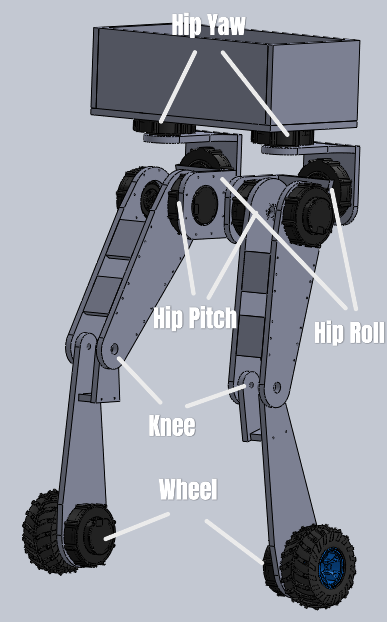
\includegraphics[width=\linewidth]{figures/annotated_robot_joints.png}
    \caption{Robot joint layout with world coordinate frame (right-handed, Z up). In the model as built, both wheel axles lie along world $X$ and the two wheel links are separated by \SI{0.271}{m} along $X$; the rolling---and therefore sagittal---direction is world $Y$, and world $X$ is the lateral (track) axis. All axis-resolved results in this paper follow that convention, verified four independent ways in Section~\ref{sec:standing}. The CoM is located at the torso geometric center. Each leg: hip roll (HR), hip yaw (HY), hip pitch (HP), knee (KN), wheel (WH).}
    \label{fig:robot}
\end{figure}

% ============================================================
\section{ACC Formulation}
% ============================================================

\subsection{Two-Channel Torque Assembly}
\label{sec:overview}

ACC assembles a PD balance core, proximity-gated anchor integral, and posture regulation into two torque channels---wheel torque ($\boldsymbol{\tau}_w\in\mathbb{R}^2$) and leg-joint torque ($\boldsymbol{\tau}_q\in\mathbb{R}^8$)---with flight and terrain as independent extensions (Fig.~\ref{fig:acc_arch}):

\begin{equation}
\begin{aligned}
\boldsymbol{\tau}_w &= \boldsymbol{\tau}_{\text{balance}} + g_{\text{anchor}}\boldsymbol{\tau}_{\text{anchor}} + g_{\text{flight}}\boldsymbol{\tau}_{\text{flight}},\\
\boldsymbol{\tau}_q &= \boldsymbol{\tau}_{\text{posture}}(h^{\text{cmd}}) + g_{\text{terrain}}\Delta\boldsymbol{\tau}_{\text{posture}}(h^{\text{cmd},L},\,h^{\text{cmd},R}).
\end{aligned}
\label{eq:two_channel}
\end{equation}

Every gate $g_*$ except the flight gate is a \emph{smoothstep} function of a physical condition (proximity, quietness, attitude, terrain disparity) rather than a discrete switch:

\begin{equation}
\operatorname{ss}(x;a,b) = 3t^2 - 2t^3,
\qquad t = \operatorname{clip}\!\left(\frac{x-a}{b-a},\,0,\,1\right).
\label{eq:smoothstep}
\end{equation}

Equation~\eqref{eq:smoothstep} is the standard Hermite blend: it is $C^1$ in $x$, with $\operatorname{ss}=0$ for $x\leq a$, $\operatorname{ss}=1$ for $x\geq b$, and zero derivative at both knees.
Continuity matters here for a concrete reason. A hard threshold on any of these conditions injects a torque step whose magnitude equals the full gated component; at \SI{100}{Hz} with a \SI{400}{Nm/s} rate limit, such a step is spread over several control cycles by the rate limiter and appears to the plant as an unmodelled impulse.
Smoothstep removes the step entirely: the gated component enters and leaves the torque sum with continuous first derivative, so the rate limiter is never the active constraint during a gate transition.
The one exception is $g_{\text{flight}}$, which is a genuinely discrete load-based hysteresis with asymmetric engage/release timers (\num{2}-step engage, \num{5}-step release); contact loss is a binary physical event, and the asymmetric timers exist specifically to prevent balance torque from re-engaging during landing bounce.
Note that the composition $g_{\text{env}} = 1 - \operatorname{ss}(\mathrm{EMA}(|v_{\text{sag}}|);\cdot)$ is only $C^0$ \emph{in time}, because the asymmetric EMA of Eq.~\eqref{eq:asym_ema} switches coefficients when $|v_t|$ crosses $\mathrm{EMA}_{t-1}$; the smoothstep is still $C^1$ in its argument, so the resulting torque is continuous but its time derivative may jump at attack/release transitions.

Wheel torques control sagittal balance and yaw; leg-joint torques control posture and per-leg height adaptation.
The two channels are coupled only through the plant, not through the controller: no term in $\boldsymbol{\tau}_w$ reads a leg-posture state and no term in $\boldsymbol{\tau}_q$ reads the sagittal balance state.
This is what allows flight recovery and terrain adaptation to be added as independent extensions (Section~\ref{sec:flight}, Section~\ref{sec:terrain}) without retuning the anchor.

\textbf{Relation to existing gated architectures.}
``Conditionally-gated'' here denotes smoothstep activation by \emph{physical} conditions ($g_{\text{prox}}$, $g_{\text{env}}$, $g_\theta$, $g_{\text{terrain}}$). Continuous blending is not itself novel---split-range, selector, and override controllers have used it in process control for decades~\cite{shinskey1996,astrom2005advanced}.
Three distinctions are worth stating precisely.
First, industrial override architectures select \emph{among parallel controllers} using process-variable limits; ACC gates \emph{components within a single torque assembly} using physical regime.
Second, the gating variables are not control errors but physical quantities of three different kinds---spatial (distance from home), temporal (velocity envelope), and safety-interlock (attitude)---each chosen because a specific measured failure mode of this platform is expressible in it (Section~\ref{sec:discussion}).
Third, ACC is not cascade control~\cite{cascade_standard}: there is no inner/outer loop hierarchy and no setpoint is passed between controllers.
The contribution is therefore the \emph{synthesis}---which gating surfaces, on which variables, with which asymmetry---not the blending mechanism.

\begin{figure}[pos=!htbp]
    \centering
    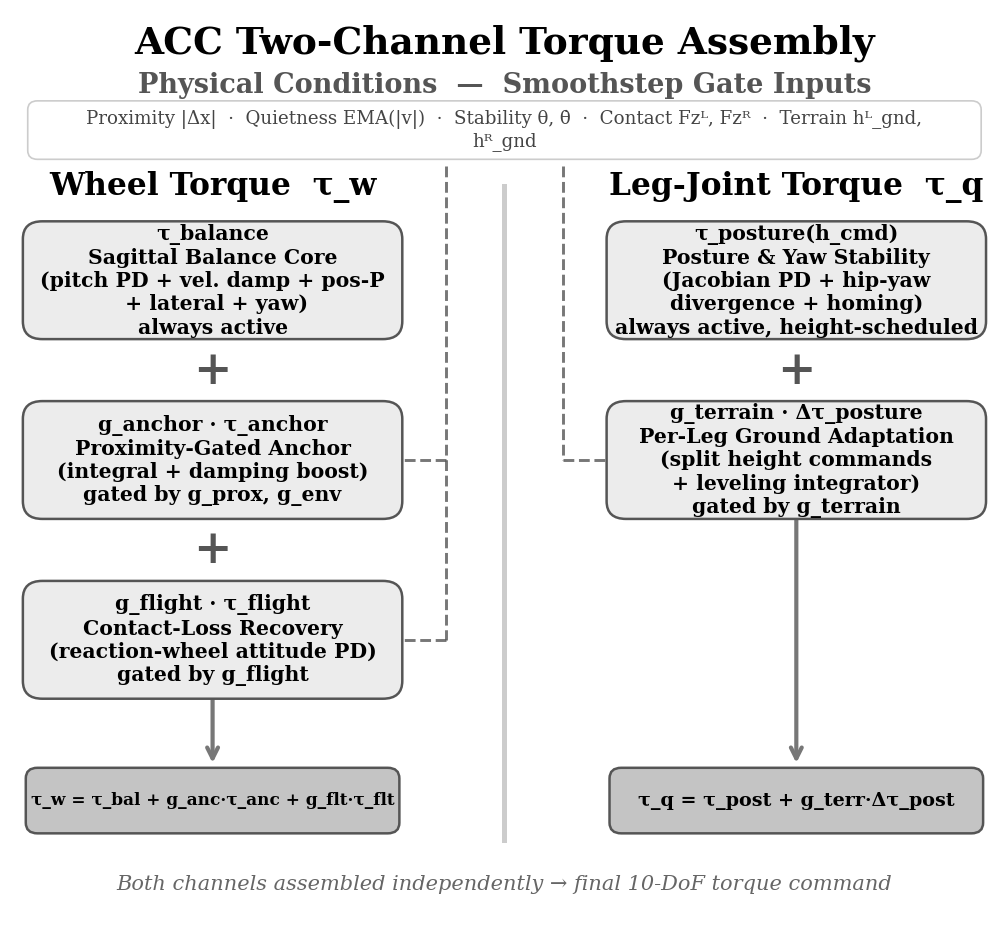
\includegraphics[width=\linewidth]{figures/acc_architecture.png}
    \caption{ACC two-channel torque assembly. Physical conditions gate each component via continuous smoothstep functions (dashed).}
    \label{fig:acc_arch}
\end{figure}

\subsection{Sagittal Balance Core ($\boldsymbol{\tau}_{\text{balance}}$)}
\label{sec:balance_core}

The sagittal balance component is always active and acts entirely in the wheel-torque channel:

\begin{equation}
\boldsymbol{\tau}_{\text{balance}} =
\begin{bmatrix}
\tau_{\text{com}} + \tau_{\text{diff}} \\
\tau_{\text{com}} - \tau_{\text{diff}}
\end{bmatrix},
\quad
\begin{aligned}
\tau_{\text{com}} &= \tau_{\text{pitch}} + \tau_{\text{damping}} + \tau_{\text{pos}},\\
\tau_{\text{diff}} &= \tau_{\text{lat}} + \tau_{\text{yaw}}.
\end{aligned}
\label{eq:balance}
\end{equation}

where $\tau_{\text{com}}$ and $\tau_{\text{diff}}$ are common-mode and differential components, respectively. The individual terms are:

\begin{align}
\tau_{\text{pitch}} &= k_p\cdot\theta + k_d\cdot\dot{\theta},\\
\tau_{\text{damping}} &= -k_{\text{vel}}\cdot v_{\text{sag}},\\
\tau_{\text{pos}} &= -k_{\text{pos}}\cdot\operatorname{clip}(\Delta x,\,\pm\SI{0.10}{m}),\\
\tau_{\text{lat}} &= k_{p,\text{roll}}\cdot\phi + k_{d,\text{roll}}\cdot\dot{\phi},\\
\tau_{\text{yaw}} &= k_{p,\text{yaw}}\cdot e_\psi + k_{d,\text{yaw}}\cdot\omega_z,
\end{align}

where $\theta$ is the torso pitch angle, $\dot{\theta}$ is the pitch rate, $v_{\text{sag}}$ is the sagittal body velocity, $\Delta x$ is the sagittal position error from the latched home position, $\phi$ is the roll angle, and $e_\psi$ is the yaw error.

\textbf{P-only limitation.}
The P position term ($k_{\text{pos}}$, clipped to $\pm\SI{0.10}{m}$, saturating at $\pm\SI{4}{Nm}$) keeps the robot within $\pm$\SIrange{4}{6}{cm} of home but leaves a \SI{1.3}{Nm} equilibrium bias sustaining a perpetual limit cycle---motivating the anchor integral.

\textbf{Why saturation-triggered anti-windup is insufficient.}
Saturation-triggered AW triggers on actuator saturation; on this platform the critical failure is \textbf{state-dependent}: during a push, position error grows to \SIrange{10}{30}{cm} while wheels remain within their \SI{20}{rad/s} range, so saturation-triggered AW never activates.
ACC's proximity gate provides spatial confinement via continuous smoothstep---avoiding both over-restriction (blocking slow-drift correction) and under-restriction (allowing windup during sustained pushes).
The simplest conditional-integration AW is evaluated in Appendix~\ref{sec:aw_supp}; broader AW families remain open.

\textbf{Pitch stiffness.}
Pitch stiffness is fixed at $k_p{=}50$ in the canonical ACC architecture. The anchor and boost alone resolve the precision-push trade-off without gain scheduling; a scheduled variant that softened $k_p$ from 50 to 35 during pushes was tested and rejected---it did not improve push survival (S0 vs.\ S1, Table~\ref{tab:push_ablation}) and is excluded from the canonical specification.

\subsection{Proximity-Gated Anchor Mechanism ($g_{\text{anchor}}\!\cdot\!\boldsymbol{\tau}_{\text{anchor}}$)}
\label{sec:anchor}

The anchor mechanism is the core contribution. It adds two terms to the wheel-torque channel that are active only when the robot is near home \emph{and} genuinely at rest:

\begin{equation}
\boldsymbol{\tau}_{\text{anchor}} =
K_i\!\int\! g_{\text{prox}}\cdot g_{\text{env}}\cdot(-\Delta x)\,dt \;+\;
g_{\text{boost}}\cdot K_{\text{boost}}\cdot(-v_{\text{sag}}),
\label{eq:anchor}
\end{equation}

where all gates are continuous smoothstep functions designed to equal $1$ when the robot is ``at home and quiet'' and transition smoothly to $0$ otherwise:

\begin{align}
g_{\text{prox}}(\Delta x) &= 1 - \operatorname{ss}\bigl(|\Delta x|;\;\SI{0.05}{m},\,\SI{0.15}{m}\bigr),
\label{eq:g_prox}\\[2pt]
g_{\text{env}}(v_{\text{sag}}) &= 1 - \operatorname{ss}\bigl(\mathrm{EMA}(|v_{\text{sag}}|);\;\SI{0.25}{m/s},\,\SI{0.50}{m/s}\bigr),
\label{eq:g_env}\\[2pt]
g_\theta(\theta,\dot{\theta}) &= \bigl[1 - \operatorname{ss}(|\theta|;\,\SI{2}{\degree},\,\SI{12}{\degree})\bigr] \nonumber\\
&\quad\times \bigl[1 - \operatorname{ss}(|\dot{\theta}|;\,\SI{2}{\degree/s},\,\SI{15}{\degree/s})\bigr],
\label{eq:g_theta}\\[2pt]
g_{\text{boost}} &= g_{\text{prox}}\cdot g_{\text{env}}\cdot g_\theta,
\label{eq:g_boost}
\end{align}

where $\operatorname{ss}(x;a,b)$ denotes the smoothstep of Eq.~\eqref{eq:smoothstep} with lower and upper knees $a$ and $b$.
Each gate is therefore a dimensionless, monotone, $C^1$ function that equals $1$ inside its ``home and quiet'' band, falls smoothly to $0$ outside it, and never switches discontinuously.
Three physically distinct conditions must hold simultaneously for the anchor to integrate: the robot must be spatially near home ($g_{\text{prox}}$), temporally quiet ($g_{\text{env}}$), and attitudinally settled ($g_\theta$).

The pitch stability gate $g_\theta$ closes when either pitch or pitch rate exceeds its band, preventing the damping boost from fighting a gentle sustained push that does not trigger the velocity envelope.
When the robot is genuinely at rest ($|\theta|<\SI{2}{\degree}$, $|\dot{\theta}|<\SI{2}{\degree/s}$), $g_\theta=1$ and the boost is fully available.

\textbf{Asymmetric envelope follower.}
The key to reliable quiet-stance detection is the asymmetric exponentially-weighted moving average (EMA) of $|v_{\text{sag}}|$:
\begin{equation}
\text{EMA}_t = \begin{cases}
\alpha_a|v_t| + (1{-}\alpha_a)\text{EMA}_{t-1}, & \text{if } |v_t| > \text{EMA}_{t-1},\\
\alpha_r|v_t| + (1{-}\alpha_r)\text{EMA}_{t-1}, & \text{otherwise},
\end{cases}
\label{eq:asym_ema}
\end{equation}
with time constants $\tau_{\text{attack}}{\approx}\SI{23}{ms}$ and $\tau_{\text{release}}{\approx}\SI{1.5}{s}$ as the primary specification; the discrete coefficients are derived via $\alpha_a=1-\exp(-\Delta t / \tau_{\text{attack}})\approx 0.35$ and $\alpha_r=1-\exp(-\Delta t / \tau_{\text{release}})\approx 0.007$ at \SI{100}{Hz} ($\Delta t{=}\SI{0.01}{s}$).
This asymmetry is essential: a symmetric EMA is \emph{bistable}---post-push oscillation holds the EMA in a middle band where the gate is half-open and the boost cannot collapse the cycle (validated by the symmetric-EMA ablation, Section~\ref{sec:results}).
The fast-attack/slow-release envelope jumps to $1$ only when oscillation truly decays, and drops to $0$ within $\sim\SI{25}{ms}$ of a disturbance. The mechanism is a peak-hold/envelope detector with asymmetric time constants; ACC's contribution is coupling envelope detection to a spatial proximity gate for integral conditioning. Fig.~\ref{fig:gate_activation} illustrates the complete gate activation sequence during a push-recovery cycle.

\textbf{EMA initialization.}
EMA$_0{=}0$ biases $g_{\text{env}}{\approx}1$ for $\sim$\SI{7.5}{s} at startup, decaying as velocity noise accumulates.
Measurements use \SIrange{3}{5}{s} settle (see Table captions); hardware should initialize $\text{EMA}_0{=}1.0$.

\begin{figure*}[pos=!tp]
    \centering
    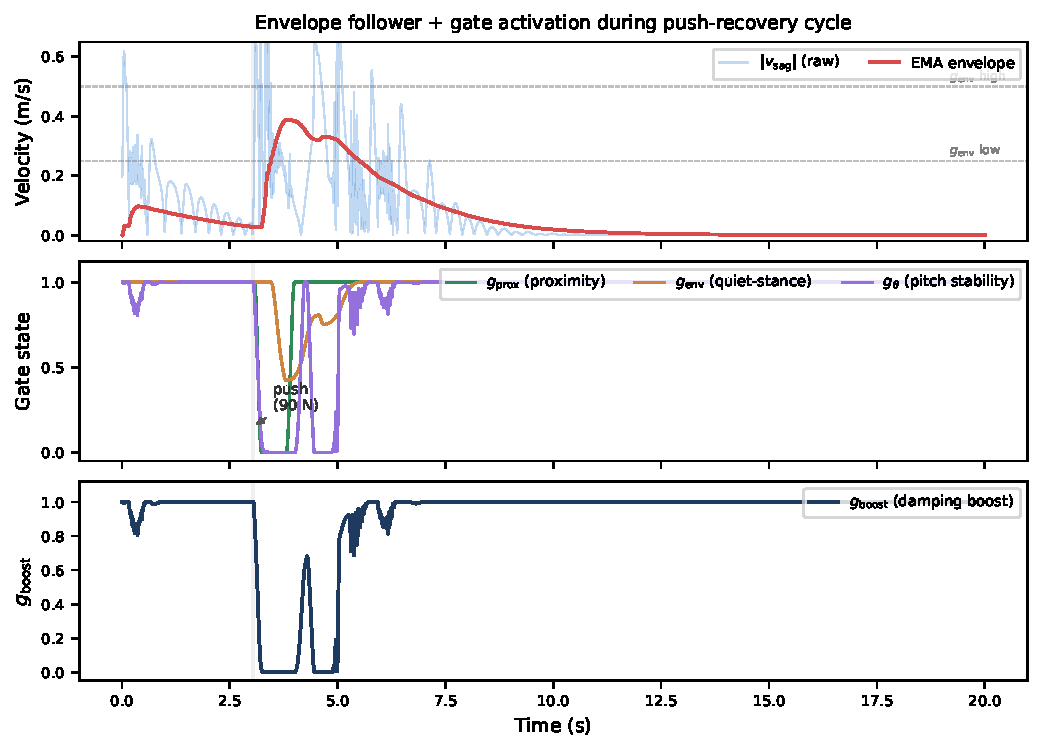
\includegraphics[width=\linewidth]{figures/gate_activation.pdf}
    \caption{Gate activation during a \SI{90}{N} lateral (world $+x$) push-recovery cycle (\SI{100}{Hz} control). \textbf{Top:} $|v_{\text{sag}}|$ and asymmetric EMA envelope; dashed lines mark the \SIrange{0.25}{0.50}{m/s} quiet-stance band. \textbf{Middle:} Individual gate states. \textbf{Bottom:} Composite damping boost $g_{\text{boost}}$. Grey shading: \num{7}-step push window. The three panels are the empirical basis for finding (iii) of Section~\ref{sec:idle_mechanism}: $g_{\text{prox}}$ and $g_{\text{env}}$ both sit pinned at their quiet-stance values before the impulse and after the ringdown, which is why ablating either reproduces ACC bit-for-bit at idle, and why only a disturbance experiment can measure their contribution.}
    \label{fig:gate_activation}
\end{figure*}

\subsection{Posture and Yaw Stability ($\boldsymbol{\tau}_{\text{posture}}$)}
\label{sec:posture}

Posture regulation uses Jacobian-based PD gains scheduled across 23 heights:

\begin{equation}
\begin{split}
\boldsymbol{\tau}_{\text{posture}} =\;&
\boldsymbol{\tau}_{\text{PD}}^{\text{jac}}(q,\dot{q},h^{\text{cmd}})
+ \boldsymbol{\tau}_{\text{div}}(q_{\text{hy}}^L,q_{\text{hy}}^R)\\
&+ g_{\text{settled}}\,\boldsymbol{\tau}_{\text{homing}}(q-q_{\text{ref}}),
\end{split}
\label{eq:posture}
\end{equation}

where $\boldsymbol{\tau}_{\text{div}}$ damps hip-yaw divergence and $\boldsymbol{\tau}_{\text{homing}}$ restores nominal posture when upright and settled.
Yaw return uses wheel-differential torque.

\subsection{Contact-Loss Recovery ($g_{\text{flight}}\!\cdot\!\boldsymbol{\tau}_{\text{flight}}$)}
\label{sec:flight}

When both wheels lose ground contact, ACC detects this via per-wheel normal forces and substitutes a flight attitude controller using the wheels as reaction flywheels:

\begin{align}
g_{\text{flight}} &= \begin{cases}
1, & \text{if } F_z^L, F_z^R < 0.5mg \text{ for } {\geq} 2 \text{ steps},\\
0, & \text{if } \min(F_z^L,F_z^R) \geq 0.5mg \text{ for } {\geq} 5 \text{ steps},
\end{cases}\\[2pt]
\boldsymbol{\tau}_{\text{flight}} &= \operatorname{clip}\!\big(2.0\theta + 0.5\dot{\theta} - 0.02\omega_{\text{wheel}},\;\pm\SI{2}{Nm}\big).
\label{eq:flight}
\end{align}

Forward wheel spin pitches nose-up during descent; \num{5}-step release
hysteresis prevents balance-torque re-engagement during bounce. The free-fall
drop is a stress test and the ledge drive-off the intended use case. The
wheel--inverted-pendulum loop this override replaces is itself a
reaction-flywheel controller once the wheels are unloaded, so the override's
measured contribution is to bound landing-attitude variance near the upper end
of the drop envelope rather than to enable recovery; Section~\ref{sec:flight_terrain_results}
(Table~\ref{tab:flight_ext}) separates the two at $N{=}10$.

\subsection{Per-Leg Ground Adaptation ($g_{\text{terrain}}$)}
\label{sec:terrain}

When the two wheels rest at different ground heights---a curb straddle, an
oblique ledge---a single torso height command forces the torso to roll by the
step angle. ACC instead maintains an \emph{independent ground estimate per leg}
and issues two height commands. The estimate is taken from the wheel
contact-point height, which is exact at any body tilt for a rigid wheel, and is
updated only while that wheel carries real load:
\begin{equation}
\hat{h}_{\text{gnd}}^{i} \leftarrow \hat{h}_{\text{gnd}}^{i}
+ \alpha_g\big(z_{\text{contact}}^{i} - \hat{h}_{\text{gnd}}^{i}\big),
\; F_z^{i} \geq 0.2mg, \; i \in \{L,R\},
\label{eq:terrain_est}
\end{equation}
with $\alpha_g = 0.35$ per control step to reject contact chatter. The
$0.2mg$ load test rather than mere geometric touching is deliberate: a lightly
touching wheel that is in the act of unloading rides a few centimetres high and
injected a \SI{+2.9}{cm} phantom ground step on the \SI{15}{cm} curb.

An unloaded wheel does \emph{not} update~\eqref{eq:terrain_est}. It freezes its
estimate, because an airborne wheel supplies no information about where its
ground is. The one exception is the only physically unambiguous
``my ground is gone'' signal---the wheel centre descending \emph{below} its own
believed ground:
\begin{equation}
\delta^{i} > \SI{3}{mm}
\;\Rightarrow\;
\dot{\hat{h}}_{\text{gnd}}^{i} = -\big(v_0 + k_s \,\delta^{i}\big),
\label{eq:terrain_seek}
\end{equation}
where $\delta^{i} = \hat{h}_{\text{gnd}}^{i} - z_{\text{contact}}^{i}$ is the
depth by which the wheel has fallen below its believed ground,
with $v_0 = \SI{0.5}{m/s}$ and $k_s = \SI{50}{\per\second}$. The
proportional term matters: a fixed slew converged the ground estimate in
\SI{0.30}{s}, by which time a \SI{20}{cm} dismount had already tipped the robot
past recovery, whereas a \SI{15}{cm} drop under~\eqref{eq:terrain_seek} slews at
\SI{8}{m/s} and converges within two control steps, so the leg extends
\emph{during} the fall rather than after it. When both wheels are airborne, both
estimates track the mean wheel height, which reproduces the symmetric
pre-adapter behaviour exactly and leaves ballistic flight to
Section~\ref{sec:flight}.

The step $\Delta h = \hat{h}_{\text{gnd}}^{L} - \hat{h}_{\text{gnd}}^{R}$ is
then absorbed by the legs rather than the torso. The split is kinematic, not a
linear height offset: with $L(\cdot)$ the forward-kinematic leg length and
$L^{-1}$ its inverse over the calibrated posture range, the leg on the higher
ground is shortened by the full step,
\begin{align}
L_{\text{high}} &= L\big(h^{\text{cmd}}\big) - |\Delta h|,\\
h^{\text{high}} &= L^{-1}\!\big(L_{\text{high}}\big), \qquad
h^{\text{low}} = h^{\text{cmd}},
\label{eq:terrain_split}
\end{align}
both clamped to the calibrated envelope extended by \SI{10}{cm} at each end. To
first order this is the familiar $h^{\text{cmd}} \mp \Delta h/2$ symmetric
split, but the $h \mapsto L$ map is markedly nonlinear near full squat: the
linear proxy erred by \SI{12}{cm} at the lower extrapolation limit, folding the
knee back under the thigh. If $L_{\text{high}}$ falls below the shortest
physically reachable leg, ACC raises the \emph{whole} robot until the short leg
fits, trading commanded height for the ability to span the step. A
\SI{20}{cm} curb at nominal stance exceeds even this: it would require
\SI{170}{\degree} of knee flexion against a \SI{2.7}{rad} limit, and the
uncompensated remainder appears as a predicted torso roll
$\arctan(-\varepsilon / w_{\text{track}})$ with $\varepsilon$ the unspanned
step and $w_{\text{track}} = \SI{0.278}{m}$ the wheel separation. Reporting
this expected roll explicitly is what keeps a legitimate straddle from being
misread as an incipient fall by the tilt-based safety monitors.

Because the $h \mapsto L$ table is itself extrapolated at the extremes, a
purely feedforward split left a systematic \SI{+6}{\degree} torso roll on the
\SI{10}{cm} curb. A closed-loop leveling integrator trims the split by the
\emph{measured} roll at \SI{0.15}{m/(rad.s)} with \SI{\pm 6}{cm} of authority.
It integrates only when all three of the following hold: both wheels loaded, a
genuine ground step $|\Delta h| \geq \SI{2}{cm}$, and a ground estimate settling
at less than \SI{0.15}{m/s}. The gating is not cosmetic. Without the step
condition, the dynamic roll of a turn is integrated as if it were terrain and
wound an \SI{8.6}{\degree} roll bias through a \SI{180}{\degree} turn; without
the rate condition, the geometric transient of a curb climb is integrated as a
leveling error and compresses the flat leg. Off-step, the trim decays to zero
with a \SI{1}{s} time constant.

The expected roll must also reach the \emph{gates}, not only the posture solver.
Heading hold is a differential wheel torque scaled by a stability envelope whose
roll factor decays over \SIrange{1}{5}{\degree}. The unspanned remainder of a
\SI{20}{cm} step is a quasi-static \SIrange{2.5}{4.0}{\degree}, so the envelope
read a legitimate straddle as an incipient fall and suppressed heading hold for
the entire crossing---the mount transient then went undamped and the robot yawed
off the slab. ACC therefore widens the roll band in proportion to the commanded
split, over the same \SIrange{3}{10}{cm} interval the wheel loop already uses,
and restores both the differential term and the mean-ground height reference once
the straddle has \emph{settled}. Settling is decided by the rate of the commanded
split against a \SI{0.2}{s} exponential average: $|\Delta \dot h|$ is
\SIrange{0.05}{0.13}{m/s} while a wheel climbs and below \SI{0.016}{m/s} once
astride, a tenfold separation. Restricting the relaxation to the settled phase is
a requirement rather than conservatism---applying it while a wheel is still
crossing an edge keeps drift authority alive over the drop and topples the robot
on a \SI{45}{\degree} oblique exit. On flat ground $\Delta h \equiv 0$ and every
term above vanishes identically.

% Platform comparison table — qualitative, not binary
\begin{table}[pos=!tbp]
\centering
\footnotesize
\caption{Capability comparison across wheeled biped platforms. ``---'' = not reported in cited work. Idle precision and push force are not standardized benchmarks; quantitative cross-platform comparison is limited by metric heterogeneity.}
\label{tab:platform_comparison}
\setlength{\tabcolsep}{2pt}\begin{tabular}{@{}>{\raggedright\arraybackslash}p{1.3cm}>{\raggedright\arraybackslash}p{1.1cm}>{\raggedright\arraybackslash}p{1.1cm}>{\raggedright\arraybackslash}p{1.1cm}>{\raggedright\arraybackslash}p{1.1cm}>{\raggedright\arraybackslash}p{1.85cm}@{}}
\toprule
Metric & Ascento & DIABLO & Whleaper & SKATER & \textbf{ACC (Ours)} \\
\midrule
Balance &
  LQR &  LQR +\newline aux.\ loops &
  LQR / PPO\newline (per mode) &
  Hierarch.\newline MPC &
  \textbf{Gated PD\newline + anchor I} \\
\addlinespace
Idle precision &
  --- &
  --- &
  --- &
  --- &
  \textbf{\SI{0.294}{mm}\newline sag.\ CoM RMS} \\
\addlinespace
Push recovery &
  ---\textsuperscript{a} &
  --- &
  --- &
  --- &
  \textbf{8-dir.,}\newline $F_{\text{med}}{=}$\,\SI{107}{N} \\
\addlinespace
Height &
  Discrete\newline jump &
  Stance\textsuperscript{b} &
  Multi-modal &
  Contin. &
  \textbf{\SIrange{0.35}{0.45}{m}}\newline CoM\textsuperscript{c} \\
\addlinespace
Flight &
  Jumping\newline (airtime) &
  --- &
  --- &
  --- &
  \textbf{Drop \SI{100}{cm},\newline ledge \SI{50}{cm}} \\
\addlinespace
Terrain &
  --- &
  --- &
  --- &
  Vision-based &
  \textbf{Per-leg\newline contact} \\
\addlinespace
\textbf{Validation} &
  Hardware &
  Hardware &
  Hardware &
  Hardware &
  \textbf{Simulation} \\
\bottomrule
\end{tabular}
\vspace{2pt}\tabnote\noindent
\textsuperscript{a}Qual.\ omnidirectional push recovery demonstrated in supplementary video; quantitative force thresholds not reported in cited work.
\textsuperscript{b}Height variation demonstrated; quantitative range not reported.
\tabnote\noindent
\textsuperscript{c}Calibrated CoM-$z$ band (Section~\ref{sec:height_convention}), $\pm\SI{5}{cm}$ about the \SI{0.404}{m} nominal, with joint targets extrapolated to \SIrange{0.254}{0.554}{m}; commanded $\pm\SI{5}{cm}$ transitions are evaluated under disturbance in Section~\ref{sec:analysis}. Not comparable to the base-$z$ ranges of the cited platforms or of our PPO reference.
\end{table}

\subsection{Complete Numerical Parameter Set}
\label{sec:parameters}

Table~\ref{tab:parameters} lists core parameters; the full set (50+ gains) is available in the supplementary material.

\begin{table}[pos=!tbp]
\centering
\footnotesize
\caption{Core numerical parameters for the ACC balance controller. All values in SI units unless noted otherwise.}
\label{tab:parameters}
\begin{tabular}{@{}p{2.8cm}rp{1.8cm}@{}}
\toprule
\multicolumn{3}{c}{\textbf{Balance Core}} \\
\midrule
$k_p$                      & 50      & Nm/rad \\
$k_d$                      & 3.0     & Nm/(rad/s) \\
$k_{\text{pos}}$           & 40      & Nm/m \\
Position clip              & $\pm$4.0 & Nm \\
$k_{\text{vel}}$           & 15      & Nm/(m/s) \\
Vel.\ damp.\ scale         & 1.5     & --- \\
$k_{\text{roll}}$          & 55      & Nm/rad \\
$k_{\text{roll},d}$        & 5.5     & Nm/(rad/s) \\
$k_{\text{yaw}}$           & 1.0     & Nm/rad \\
$k_{\text{yaw},d}$         & 0.3     & Nm/(rad/s) \\
$k_{\text{pos,return}}$    & 2.0     & Nm/m \\
$k_{\text{heading}}$       & 2.0     & Nm/rad \\
$k_{\text{heading},d}$     & 0.6     & Nm/(rad/s) \\
\addlinespace
\multicolumn{3}{c}{\textbf{Anchor Mechanism}} \\
\addlinespace
$K_i$ (anchor integral)    & 4.0     & Nm/(m$\cdot$s) \\
Integral cap               & 2.0     & Nm \\
Integral leak              & 5$\times$10$^{-3}$ & per step \\
Boost scale $k_{\text{vb}}$& 5.0     & --- \\
$g_{\text{prox}}$ band     & 0.05--0.15 & m \\
$g_{\text{env}}$ band      & 0.25--0.50 & m/s \\
$\tau_{\text{attack}}$     & 0.023   & s \\
$\tau_{\text{release}}$    & 1.5     & s \\
$g_{\text{stab}}$ ($\theta$) & 2--12  & $^\circ$ \\
$g_{\text{stab}}$ ($\dot{\theta}$) & 2--15 & $^\circ$/s \\
\addlinespace
\multicolumn{3}{c}{\textbf{Flight / Terrain / Other}} \\
\addlinespace
$k_{\text{flight}}$ (P / D)& 2.0 / 0.5 & --- \\
Wheel damping (flight)     & 0.02    & Nm/(rad/s) \\
Flight engage / release    & 2 / 5   & steps \\
\makecell[l]{$F_z$ thresh.\\(flight / terrain)} & 0.5 / 0.2 & $\times mg$ \\
\bottomrule
\end{tabular}
\vspace{2pt}\tabnote\noindent
\end{table}

% ============================================================
\section{Experimental Validation}
\label{sec:results}
% ============================================================

We evaluate ACC across four scenario classes, each mapped to the component it tests and paired with targeted ablations.
ACC and all six classical baselines are evaluated at \SI{500}{Hz} simulation / \SI{100}{Hz} control, so the headline comparison is rate-matched by construction. The PPO reference is reported at the \SI{50}{Hz} rate its policy was trained at. All configurations use a \SI{400}{Nm/s} torque rate limit per joint.

\emph{Control rate.} Every classical baseline was measured at two control rates under an otherwise identical protocol, with episode length held fixed in seconds rather than in steps: ACC's \SI{100}{Hz}, which is what Table~\ref{tab:lqr_baselines} reports, and \SI{50}{Hz}, the rate for which the gains were tuned. Both sets appear side by side in Section~\ref{sec:rate_matched} (Table~\ref{tab:rate_matched}). The fall rate is \SI{100}{\percent} in all twelve cells, so the comparison does not turn on which rate is chosen. The converse direction---ACC at \SI{50}{Hz}---is a negative result: with the discrete coefficients recomputed for the longer step ($\alpha_a{\approx}0.58$ and $\alpha_r{\approx}0.013$, re-derived from Eq.~\eqref{eq:asym_ema} at $\Delta t{=}\SI{0.02}{s}$, with the anchor leak rescaled to \num{0.010} per step) the controller is not preserved. The robot collapses, and the mean CoM height over the recorded window is \SI{0.124}{m} against a nominal standing height of \SI{0.404}{m}. The $\SI{0.050}{mm}$ ``idle RMS'' and the \SI{10}{N} push threshold produced by that run are artifacts of a robot lying motionless on the ground---\SI{10}{N} is the lower bound of the binary search, returned when even the smallest tested impulse fails. No \SI{50}{Hz} ACC result is therefore reported, and rate-independence in the downward direction is not claimed; this is analysed as Limitation~2.
RNG seeds are deterministic: idle standing uses $\text{seed} = 20260727 + \text{trial\_id}$; push ablation uses $\text{seed} = 20260728 \times 100 + \text{rep}$; LQR baselines cycle seeds $\{0, 42, 123\}$ across episodes.

\subsection{Anchored Standing}
\label{sec:standing}

\subsubsection{Two precision metrics, deliberately kept separate}

``Standing precision'' names two different quantities in the wheeled-biped
literature, and they are not interchangeable. Let $\mathbf{p}(t)\in\mathbb{R}^2$ be
the horizontal base position over an evaluation window of length $T$, let
$\mathbf{p}_0$ be the commanded home position, and let
$\bar{\mathbf{p}}=\frac{1}{T}\int_0^T\mathbf{p}(t)\,dt$ be the trial mean. We report

\begin{align}
A &= \Bigl(\tfrac{1}{T}\textstyle\int_0^T \lVert\mathbf{p}(t)-\mathbf{p}_0\rVert^2\,dt\Bigr)^{1/2},
\label{eq:accuracy}\\
R &= \Bigl(\tfrac{1}{T}\textstyle\int_0^T \lVert\mathbf{p}(t)-\bar{\mathbf{p}}\rVert^2\,dt\Bigr)^{1/2}.
\label{eq:repeatability}
\end{align}

$A$ is the \emph{accuracy}: RMS displacement from the position the controller was
told to hold. It retains any DC parking offset, so it answers ``how close to the
commanded pose does the robot actually park?''. $R$ is the \emph{repeatability}:
RMS about the trial's own mean, with the DC offset removed. It answers ``how still
is the robot once it has parked?''. A controller with a persistent \SI{27}{mm}
offset and a perfectly steady hold scores $A{=}\SI{27}{mm}$ but
$R{\approx}\SI{0}{mm}$; a controller centred on the target but oscillating scores
the reverse. Reporting either alone is uninformative, and---because the two differ
by more than an order of magnitude on this platform---comparing a value of one
against a value of the other produces a meaningless ratio.

Both are reported for every configuration below, resolved separately along the
sagittal axis, the lateral axis, and the full plane, because the two horizontal
axes of this platform are not merely different in degree---they are actuated by
different means and must not be pooled or interchanged. We therefore fix the
convention explicitly, since the two are easy to transpose and the physical
conclusions invert if they are:

\begin{itemize}
\item The \textbf{sagittal} axis is world $y$. Both wheel axles point along world
$x$ and the two wheels are separated along world $x$
($w_{\text{track}}{=}\SI{0.278}{m}$), so the rolling direction---the axis on
which wheel torque produces ground force, and the only axis with a genuine
inverted-pendulum mode---is world $y$. The controller agrees: \verb|init_v3_controller|
packs $\hat{\mathbf{s}}=(0,1)$ as its sagittal unit vector.
\item The \textbf{lateral} axis is world $x$. No actuator produces lateral ground
force; the axis is held passively by the wheel contacts and by the roll restoring
moment of the track width.
\end{itemize}

\noindent Two dynamic checks confirm the assignment rather than merely asserting
it. A \SI{90}{N} impulse along $y$ is absorbed with a peak wheel speed of
\SI{52}{rad/s} and leaves a residual offset of \SI{4.8}{mm}---the wheels drive
back under the CoM---whereas the same impulse along $x$ leaves a permanent
\SI{23.2}{mm} offset at a peak wheel speed of \SI{18}{rad/s}, because nothing can
push the robot sideways again. And over a \SI{20}{s} quiet stance the robot rolls
\SI{24.6}{mm} along $y$ with the wheel midpoint tracking the CoM to within
\SI{0.2}{mm}, while $x$ holds to \SI{0.02}{mm}. All four checks are reproduced by
\texttt{scripts/verify\_body\_axes.py}, which asserts on disagreement.

This matters for reading Table~\ref{tab:standing}: the anchor integral and the
gated damping boost both live in the wheel-torque channel, so \emph{both act on
the sagittal axis only}. The lateral column is therefore a measure of how little
the plant moves when nothing drives it, not a measure of controller quality, and
the sagittal and planar columns carry essentially all of the information about
what ACC does (Appendix~\ref{sec:parking_supp}).

\subsubsection{Unified measurement protocol}

Every row of Table~\ref{tab:standing} was re-measured under one protocol so that no
two entries in the same column come from different definitions.
Each trial runs \SI{25}{s} at \SI{500}{Hz} physics / \SI{100}{Hz} control from the
nominal standing pose with randomized initial conditions
($\sigma{=}\SI{0.005}{rad}$ per joint, clipped to joint limits;
$\sigma{=}\SI{1}{mm}$ on root height), seeded
$\text{seed}{=}20260727{+}\text{trial\_id}$ for $\text{trial\_id}\in[0,10)$.
The first \SI{5}{s} are discarded as settling---long enough to cover the
EMA$_0{=}0$ transient (${\sim}\SI{7.5}{s}$ to full release, but ${<}\SI{5}{s}$ to
within \SI{1}{\percent} of the quiet-stance value)---and $A$ and $R$ are computed
over the remaining \SI{20}{s}. Displacements are taken relative to each trial's own
$t{=}0$ pose, so $\mathbf{p}_0$ is the commanded home rather than the world origin.
A trial is scored as a fall if $|\theta|{>}\SI{46}{\degree}$ or root height
${<}\SI{0.15}{m}$ at any point. Confidence intervals are Student-$t$
($t_{9,0.025}{=}2.262$, $\text{SEM}{=}\text{SD}/\sqrt{10}$).

The protocol has one clear scope limit: because every trial starts at the
commanded home, it never exercises the anchor's return-to-home function. It
measures the controller's ability to \emph{stay} put, not to \emph{come back}. The
latter is measured by the push experiments of Section~\ref{sec:push}. This distinction
turns out to matter for attributing the mechanism (Section~\ref{sec:idle_mechanism}).

\begin{table*}[pos=!tp]
\centering
\caption{Idle standing precision across the full ablation ladder. All rows re-measured under the single protocol of Section~\ref{sec:standing}; values are mean${\pm}$SD over $N{=}10$ trials. See the note below the table for column definitions.}
\label{tab:standing}
\setlength{\tabcolsep}{2pt}
\footnotesize
\begin{tabular}{@{}ll S[table-format=2.3(4)] S[table-format=2.3(3)] S[table-format=2.3(4)] S[table-format=-2.1] S[table-format=2.3(4)] c@{}}
\toprule
& \multirow{2}{*}{Configuration}
& {$R_{\text{sag}}$ (mm)} & {$R_{xy}$ (mm)} & {$R_{\text{lat}}$ (mm)} & {$\bar{s}$ (mm)} & {$A_{\text{lat}}$ (mm)} & Survival \\
& & {sagittal rep.} & {planar rep.} & {lateral rep.} & {sag.\ offset} & {lateral acc.} & \\
\midrule
\multicolumn{8}{@{}l}{\textbf{Additive ladder (bottom-up)}}\\
L0   & P-only (PD, no position, no integral) & 17.461(258) & 17.845(279) & 3.675(246) & -44.8 & 9.933(712) & 10/10 \\
L1   & $+$ position homing ($\pm\SI{0.10}{m}$) & 20.397(17) & 20.414(19) & 0.834(66) & -30.4 & 2.629(884) & 10/10 \\
L2   & $+$ ungated integral $K_i$ & 25.026(39) & 25.056(43) & 1.212(110) & -27.5 & 3.661(1264) & 10/10 \\
L2.5 & $+$ proximity gate only (no envelope, no boost) & 25.198(17) & 25.227(20) & 1.205(99) & -27.6 & 4.023(1194) & 10/10 \\
\addlinespace
\multicolumn{8}{@{}l}{\textbf{Proposed controller}}\\
L3/S1 & \textbf{ACC} (full anchor, fixed $k_p{=}50$) & \bfseries 0.294(15) & \bfseries 0.788(69) & \bfseries 0.730(73) & \bfseries -27.0 & \bfseries 1.213(554) & \textbf{10/10} \\
\addlinespace
\multicolumn{8}{@{}l}{\textbf{Subtractive ablation (top-down from ACC)}}\\
S0 & ACC $+$ scheduled $k_p$ (rejected variant) & 0.294(15) & 0.788(69) & 0.730(73) & -27.0 & 1.213(554) & 10/10 \\
S2 & $-$ gated damping boost & 4.772(69) & 4.824(67) & 0.703(69) & -26.8 & 1.260(616) & 10/10 \\
S3 & $-$ asymmetric envelope (symmetric EMA) & 0.294(15) & 0.788(69) & 0.730(73) & -27.0 & 1.213(554) & 10/10 \\
S4 & $-$ proximity gate (integral always on) & 0.294(15) & 0.788(69) & 0.730(73) & -27.0 & 1.213(554) & 10/10 \\
S5 & $-$ pitch safety gate $g_\theta$ & {---} & {---} & {---} & {---} & {---} & \textbf{0/10} \\
\addlinespace
\multicolumn{8}{@{}l}{\textbf{Single-mechanism isolation (ACC with one term disabled)}}\\
M1 & $K_i{=}0$ (anchor integral removed, gates intact) & 0.089(35) & 0.733(72) & 0.727(71) & -31.2 & 1.192(535) & 10/10 \\
M2 & damping terms reverted to their L2 values & 25.198(17) & 25.227(20) & 1.205(99) & -27.6 & 4.023(1194) & 10/10 \\
M3 & $K_i{=}0$ \emph{and} boost $=0$ & 3.973(130) & 4.037(128) & 0.710(69) & -31.1 & 1.241(591) & 10/10 \\
\bottomrule
\end{tabular}
\vspace{2pt}\tabnote\noindent
\textbf{Protocol.} $N{=}10$ trials, \SI{100}{Hz} control, \SI{20}{s} measurement
window after a \SI{5}{s} settle, clean sensors, \SI{0}{ms} actuator delay.

\noindent\textbf{Columns.} $R$ = repeatability (RMS about the trial mean,
Eq.~\eqref{eq:repeatability}); $A$ = accuracy (RMS from commanded home,
Eq.~\eqref{eq:accuracy}); $\bar{s}$ = mean signed sagittal parking offset.
Sagittal is world $y$ and lateral is world $x$ (Section~\ref{sec:standing}). The
anchor integral and the damping boost act on the sagittal axis only, so
$R_{\text{sag}}$ and $\bar{s}$ are the columns that discriminate between
configurations, while $R_{\text{lat}}$ measures a passively held axis and is
near-constant by construction.

\noindent\textbf{Omitted columns.} $A_{\text{sag}}$ and $A_{xy}$ carry no
information beyond the columns shown: over all twelve surviving rows the
identities $A_{\text{sag}}=\sqrt{\bar{s}^{2}+R_{\text{sag}}^{2}}$ and
$A_{xy}=\sqrt{A_{\text{sag}}^{2}+A_{\text{lat}}^{2}}$ hold to \SI{0.003}{mm}
and \SI{0.02}{mm} respectively---accuracy on an axis is just that axis's
parking offset and its repeatability added in quadrature.

\noindent Produced by \path{scripts/collect_idle_ladder.py} (per-trial worker
\path{scripts/_idle_ladder_worker.py}); raw output
\path{outputs/paper_verification/idle_ladder.json}.
\end{table*}

\subsubsection{Result}

ACC holds \textbf{sub-millimeter sagittal repeatability},
$R_{\text{sag}} = 0.294{\pm}\SI{0.015}{mm}$ (95\%\,CI $[0.283,0.305]$\,mm), across
ten randomized trials with no falls. This is the figure of merit for the platform,
because sagittal is the actuated inverted-pendulum axis: it is the axis on which
the robot can fall, the axis the wheel-torque channel drives, and the axis that
every configuration in the ladder is trying to hold.

Signal-to-noise ratios against a pinned-base simulator noise floor are not
reported: pinning zeroes velocities without welding the base, so the floor it
yields is meaningful on the laterally constrained axis (\SI{0.0019}{mm} RMS) but
not on the gravity-loaded ones. Precision is therefore assessed from the relative spread
\emph{between} configurations measured under an identical protocol: removing a
single mechanism (S2) moves $R_{\text{sag}}$ from \num{0.294} to
\SI{4.772}{mm}, a factor of \num{16} with non-overlapping SDs, which
establishes that the metric resolves the effect under study.

Against the P-only baseline (L0), which sustains the \SI{69.7}{mm} peak-to-peak
sagittal limit cycle described in Section~\ref{sec:intro}, the like-for-like
improvements are

\begin{itemize}
\item sagittal repeatability $R_{\text{sag}}$: $17.461 \rightarrow \SI{0.294}{mm}$, a factor of \textbf{59.4};
\item planar repeatability $R_{xy}$: $17.845 \rightarrow \SI{0.788}{mm}$, a factor of \textbf{22.6};
\item lateral repeatability $R_{\text{lat}}$: $3.675 \rightarrow \SI{0.730}{mm}$, a factor of \textbf{5.0}.
\end{itemize}

The ordering of these three factors is itself informative and worth stating
plainly, because it is the opposite of what a reader might expect. The largest
gain is on the sagittal axis, which is the hard axis; the smallest is on the
lateral axis, which is the easy one. That is the correct signature for a
wheel-torque controller: every term ACC adds beyond L0---position homing, the
anchor integral, the gated damping boost---produces ground force along the
rolling direction and none of them can produce lateral force at all. The residual
$5{\times}$ lateral improvement is an indirect consequence of the robot pitching
and yawing less rather than of any lateral control action.
A reader comparing against platforms that report a single scalar ``standing
precision'' should compare against $R_{\text{sag}}$, not against
$R_{\text{lat}}$ or a planar norm, since the latter two are diluted by an axis
this class of platform does not actuate.

\emph{Accuracy and repeatability are distinct quantities on this axis, and both
are reported.} ACC parks at $\bar{s}={-}\SI{27.0}{mm}$ from the commanded home
along the sagittal axis and holds that standoff to within \SI{0.009}{mm} SD
across trials: the settle is highly reproducible, and it terminates at a fixed
offset rather than at the commanded point. Planar accuracy is therefore
$A_{xy}=\SI{26.994}{mm}$, a $1.8{\times}$ improvement over L0
($49.1\rightarrow\SI{27.0}{mm}$) against the $59{\times}$ gain in repeatability.
The offset lies on the axis the anchor integral does control---it is neither a
measurement artifact nor an unregulated direction---and the integral moves it
from \SI{31.2}{mm} (M1, $K_i{=}0$) to \SI{27.0}{mm}. Reporting it separately
from a planar average is what makes the two quantities individually
interpretable.
Its magnitude is fully accounted for. Appendix~\ref{sec:parking_supp}
instruments the sagittal torque balance and predicts the offset in closed form
from two settings: a \emph{leaky} anchor integral, whose ${\sim}\SI{2}{s}$
forgetting horizon fixes its DC gain at
$k_{I,\text{dc}}{=}\SI{7.96}{Nm/m}$---a finite value, so a constant load leaves
a finite error by construction---and a \SI{1.44}{\degree} error in the
feedforward pitch reference. The prediction is \SI{24.88}{mm} against
\SI{24.99}{mm} measured, and it holds across a $40{\times}$ gain sweep and a
five-point height sweep to within \SI{0.92}{\percent}. The leak also buys the
steadiness: a $10{\times}$ smaller $\lambda$ cuts the offset to \SI{-16.31}{mm}
but degrades window jitter twelvefold ($0.298\rightarrow\SI{3.463}{mm}$). What
Table~\ref{tab:standing} publishes is therefore a quantified and deliberately
chosen point on that trade-off, with both alternatives priced against the full
evaluation suite (Appendix~\ref{sec:parking_supp}).

\subsubsection{Which mechanism produces the precision}
\label{sec:idle_mechanism}

The bottom two blocks of Table~\ref{tab:standing} isolate the contributions. Four
findings are worth stating precisely, because three of them contradict the
attribution that the gate structure invites.

\emph{(i) Idle steadiness comes from the damping ladder; the integral buys
accuracy instead.} The two contributions separate cleanly once the axes are kept
apart, and they do not compete for the same metric.

M1 disables the anchor integral entirely ($K_i{=}0$) while leaving every gate in
place, and its \emph{repeatability} is not merely as good as ACC's but slightly
better ($R_{\text{sag}}$ \SI{0.089}{mm} vs.\ ACC's \SI{0.294}{mm};
$R_{xy}$ \SI{0.733}{mm} vs.\ \SI{0.788}{mm}). Its \emph{accuracy}, however, is
worse by \SI{4.2}{mm}: it parks at $\bar{s}={-}\SI{31.2}{mm}$ against ACC's
$-\SI{27.0}{mm}$. That is the integral's entire measurable idle signature, and it
is exactly the trade one expects from an integral term---it walks the robot
closer to the commanded home at the cost of a small amount of steadiness, since
the accumulating term is itself a slowly-varying command. A protocol that reports
repeatability alone will conclude, wrongly, that the anchor integral is inert at
idle; a protocol that reports accuracy alone will miss that it costs a factor of
three in steadiness.

Conversely M2 keeps the integral and every gate but reverts the two
velocity-damping coefficients to their L2 values, and reproduces the L2/L2.5 limit
cycle exactly ($R_{\text{sag}}=\SI{25.198}{mm}$). Steadiness is therefore
attributable to the damping terms, in two stages: raising the velocity-damping
scale takes $R_{\text{sag}}$ from \SI{25.2}{mm} to \SI{3.97}{mm} (M3, boost still
off), and enabling the gated damping boost takes it from \SI{3.97}{mm} to
\SI{0.294}{mm} (ACC)---a combined factor of \num{86} decomposed into factors of
${\sim}\num{6.3}$ and ${\sim}\num{13.5}$. S2 confirms the second stage
independently from the top down: removing only the boost degrades
$R_{\text{sag}}$ from \SI{0.294}{mm} to \SI{4.772}{mm}.

\emph{(ii) The damping boost acts sagittally, as it must.} S2 degrades sagittal
repeatability by a factor of \num{16} ($0.294\rightarrow\SI{4.772}{mm}$) while
leaving lateral repeatability statistically unchanged
($R_{\text{lat}}=\SI{0.703}{mm}$ vs.\ ACC's \SI{0.730}{mm}, overlapping CIs). This
is the only outcome consistent with the architecture: the boost multiplies a
velocity-damping coefficient inside the wheel-torque channel
(Eq.~\eqref{eq:balance}), and wheel torque generates ground force along the
rolling direction only. The residual oscillation it suppresses is therefore a
sagittal pitching/rolling-forward mode, and an evaluation that reported the
lateral axis alone would conclude, wrongly, that the boost does nothing at idle.
The distinction matters because the lateral column is the one that reads as a
plausible ``$x$-axis RMS'' to report by default, yet it is the one column in
Table~\ref{tab:standing} that is nearly blind to every mechanism in the ladder:
across all twelve surviving configurations $R_{\text{lat}}$ spans only
\SIrange{0.70}{3.68}{mm}, and across the seven rows that retain the full damping
ladder (S0--S4, M1, M3) only \SIrange{0.70}{0.73}{mm}.

\emph{(iii) The proximity gate and the asymmetric envelope are inert during quiet
stance.} S4 (proximity gate removed) and S3 (symmetric envelope) are
\emph{bit-identical} to ACC on every idle metric. This is the expected behavior
rather than a null result: during quiet stance the base never leaves the \SI{5}{cm}
inner band, so $g_{\text{prox}}{\equiv}1$ and gating it changes nothing; and the
velocity envelope never rises into the attack branch, so the asymmetric and symmetric
followers produce the same signal. Both mechanisms are defined by what they do when
the robot is \emph{displaced}---windup prevention during a push (S4) and ringdown
after one (S3)---and are correctly evaluated only in Table~\ref{tab:push_ablation}.
The idle protocol, which starts at home and stays there, is blind to both by
construction.

\emph{(iv) The pitch safety gate is required even to stand.} S5 falls in
\num{10}/\num{10} trials during pure quiet stance, with no push applied. Removing
$g_\theta$ leaves the damping boost free to act on the pitch state at large
excursions, and the resulting positive feedback diverges from the ${\pm}\SI{0.005}{rad}$
initial perturbation alone. $g_\theta$ is therefore a stability precondition of
the quiet-stance configuration itself, not only a disturbance-time safeguard.

Taken together: the anchor's \emph{gates} are what make an aggressive damping and
integral configuration admissible without windup or divergence, while the damping
terms they admit are what deliver the steadiness. The gates are enabling
conditions rather than the proximate cause of the precision. The integral's primary role is drift rejection
under disturbance, which by construction cannot appear in a protocol that starts
at the target; its measurable idle signature is confined to the \SI{4.2}{mm}
reduction in sagittal parking offset noted above (M1 $-31.2$ vs.\ ACC
$\SI{-27.0}{mm}$), bought at a $3{\times}$ cost in sagittal repeatability. Both
effects sit on the sagittal axis, and neither is visible on the lateral one.

Post-push velocity ringdown decays within \SI{9}{s} under ACC, whereas P-only
oscillates indefinitely because the \SI{1.3}{Nm} equilibrium bias sustains the limit
cycle. The symmetric-EMA ablation exhibits bistable failure: a post-push cycle holds
the envelope at ${\approx}0.10$, leaving the boost gate half-open, and the robot
oscillates perpetually. The ungated-integral ablation winds up during the push and
prevents recovery entirely. All three of these are post-push behaviors and are
quantified in Section~\ref{sec:push}.

\subsection{Omnidirectional Push Recovery}
\label{sec:push}

Push recovery is evaluated via polar sweep: \SIrange{10}{160}{N} impulses (\num{7} control steps) at the torso in \num{8} directions.
Bearings are applied in the world frame as $\mathbf{f}=F(\cos\theta,\sin\theta,0)$, so $\theta{=}\pm\SI{90}{\degree}$ are the sagittal (fore/aft) bearings and $\theta{=}\SI{0}{\degree}/\SI{180}{\degree}$ the lateral ones, per the axis convention of Section~\ref{sec:standing}.
$F_{\min}$ is the maximum magnitude survived in \emph{every} direction; $F_{\text{med}}$ is the median.
All thresholds measured via binary search over $[\SI{10}{N},\SI{160}{N}]$ (\num{8} iterations per direction, \SI{5}{N} tolerance).
Survival: torso pitch $<\SI{46}{\degree}$ for \SI{17}{s} post-push.

\emph{The envelope is anisotropic by construction.} The two lateral bearings average \SI{98.2}{N} against \SI{131.3}{N} for the two sagittal ones, and the weakest bearing of all is the oblique \SI{45}{\degree} ($\SI{82.3}{N}$, \SI{23}{\percent} below $F_{\text{med}}$). The asymmetry follows from the morphology rather than from tuning: the wheels can drive the contact patch back under the CoM along the sagittal axis, but produce no lateral ground force at all, so lateral recovery falls to the leg and torso alone. The oblique bearings are weakest because neither mechanism has full authority there. Raising the lateral bearing therefore requires a centralized lateral task (Section~\ref{sec:wbc}), not a gain change.

\emph{The envelope is also chiral, and the chirality is in the controller.}
Superposed on the structural anisotropy is a left--right asymmetry:
$\SI{135}{\degree}$ survives \SI{40.3}{N} more than $-\SI{135}{\degree}$
(Fig.~\ref{fig:push_polar}). The plant cannot produce it. Mirroring the model
about the sagittal plane reproduces its own mass, inertia and geometry to
\SI{0.05}{mm} and \num{1e-7} respectively, so the open-loop system is
mirror-symmetric to numerical precision. Fitting
$F(\theta){=}a_0{+}a_1\cos\theta{+}b_1\sin\theta{+}a_2\cos2\theta{+}b_2\sin2\theta$
localizes the violation: a mirror symmetry forbids $b_1$ and $b_2$, a
\ang{180} rotation forbids $a_1$ and $b_1$. The measured envelope has
$b_1{=}\SI{0.3}{N}$---rotational symmetry is intact---but
$b_2{=}\SI{-16.3}{N}$, an order of magnitude above the between-episode
dispersion. The closed loop is thus $C_2$-equivariant and mirror-broken, which
is a signature of the control law, not of the geometry.
Its source is the sign convention of the two differential channels. Feeding the
controller a state and its mirror image, the commanded torque should map to its
own mirror image; it does so \emph{exactly} (\SI{0.000}{Nm} residual) on
hip-pitch, knee and wheel, and fails only on hip-roll (\SI{3.275}{Nm}, exactly
twice that channel's own \SI{1.633}{Nm} command) and hip-yaw (\SI{0.526}{Nm}).
Both are assembled antisymmetrically, $\tau_{\text{L}}{=}{+}m$,
$\tau_{\text{R}}{=}{-}m$---the right structure for a differential command, but
even rather than odd under the mirror map, so the pair commands the
same-signed torques where the mirror requires opposite-signed ones. Two
control experiments close the loop causally: mirroring those channels flips
$b_2$ from \SI{-16.2}{N} to \SI{+15.6}{N} at unchanged magnitude, while a sham
mirror that permutes the same quantities without touching the sign convention
leaves it at \SI{-15.7}{N}; and inverting the hip-roll sign alone collapses
$b_2$ to \SI{+1.2}{N}. The effect is therefore diagnosed rather than
merely observed. We report it without adopting a correction: removing the
chirality redistributes the envelope without enlarging it
($F_{\min}$ \SI{82.5}{}${\rightarrow}\SI{79.7}{N}$ in the sign-inverted arm),
so it is a property to be understood before porting the gains to a different
track width, not a defect with a free fix.\footnote{Sweep:
\path{scripts/sweep_push_chirality.py} ($N{=}5$ per bearing, four arms), raw
output \path{outputs/push_chirality/}. The $b_2$ of that sweep's shipped arm
(\SI{-16.2}{N}) and of row S1 of Table~\ref{tab:push_ablation}
(\SI{-16.3}{N}) agree, although the two use different seeds and settle
protocols.}

\emph{Single-bearing protocol.} Several auxiliary experiments---the robustness sweep (Table~\ref{tab:robustness}), the rate-limit sweep, the ringdown and gate-activation traces (Figs.~\ref{fig:gate_activation},~\ref{fig:ringdown}) and the compound-disturbance protocol (Table~\ref{tab:compound})---apply a single impulse along world $+x$ rather than repeating the full \num{8}-bearing sweep at eightfold cost. That bearing is \emph{lateral} and below median: the polar sweep places $\SI{0}{\degree}$ at $\SI{95.6}{N}$, third-weakest of the eight and \SI{11.1}{N} below $F_{\text{med}}$. Those experiments are therefore conservative probes of ACC's disturbance margin, and they are labelled lateral throughout rather than ``forward.'' The omnidirectional figures ($F_{\min}$, $F_{\text{med}}$) characterize the full envelope.

% [!tbp], not [t]: with its caption and note block this float is 648.5pt tall in
% a 672pt column, so 1-\textfraction leaves no room and plain [t] can never place
% it. Without a p fallback it stuck at the head of the deferred list and every
% later table queued behind it, to be flushed after the bibliography.
\begin{table}[pos=!tbp]
\centering
\footnotesize
\caption{Factorial ablation of ACC components: push-recovery and ringdown metrics. Clean sensors, all rows $N{=}10$, mean${\pm}$std. See the note below the table for definitions and significance tests.}
\label{tab:push_ablation}
\setlength{\tabcolsep}{3pt}\begin{tabular}{@{}c>{\raggedright\arraybackslash}p{3.1cm}rr>{\raggedright\arraybackslash}p{1.5cm}@{}}
\toprule
& Configuration & $F_{\min}$ (N) & $F_{\text{med}}$ (N) & Ringdown \\
\midrule
\multicolumn{5}{@{}l}{\textbf{Additive (bottom-up)}} \\
\addlinespace
L0 & P-only (PD, no pos., no I)  & 70.0${\pm}$1.0 & 122.1${\pm}$2.1 & never \\
L1 & $+$\,Pos.\ homing ($\pm$\SI{0.10}{m}) & 74.8${\pm}$0.8 & 130.5${\pm}$1.2 & never \\
L2 & $+$\,Integral $K_i$ (no gate) & 74.8${\pm}$1.0 & 131.1${\pm}$1.1 & --- \\
L2.5 & $+$\,Prox.\ gate only (no EMA, no boost) & 75.3${\pm}$0.8 & 131.9${\pm}$2.4 & --- \\
L3 & $+$\,Full anchor (gate, EMA, boost)\textsuperscript{7} & \bfseries 82.3${\pm}$2.2 & 106.7${\pm}$7.0 & \textbf{\SI{9.0}{s}} \\
\addlinespace
\multicolumn{5}{@{}l}{\textbf{Subtractive (top-down from ACC)}} \\
\addlinespace
S0 & ACC $+$ scheduled $k_p$ (rejected)\textsuperscript{6}  & 81.0${\pm}$2.2 & 109.2${\pm}$7.6 & \SI{9.0}{s} \\
S1 & \textbf{ACC}\textsuperscript{6} (canonical, fixed $k_p{=}50$) & \bfseries 82.3${\pm}$2.2 & 106.7${\pm}$7.0 & \textbf{\SI{9.0}{s}} \\
S2 & $-$Damping boost           & 80.8${\pm}$0.9 & 116.2${\pm}$5.3 & never\textsuperscript{1} \\
S3 & $-$Asym.\ EMA (sym.\ EMA)  & 81.6${\pm}$1.8 & 106.2${\pm}$6.7 & never\textsuperscript{2} \\
S4 & $-$Prox.\ gate (global I)  & 80.5${\pm}$2.7 & 109.2${\pm}$7.6 & windup\textsuperscript{3} \\
S5 & $-$Pitch gate $g_\theta$   & ${<}10$\textsuperscript{5} & ${<}10$\textsuperscript{5} & never\textsuperscript{4} \\
\bottomrule
\end{tabular}
\vspace{2pt}\tabnote\noindent
$F_{\min}$ and $F_{\text{med}}$ are the minimum and median survivable push over \num{8} bearings, each located by binary search to \SI{5}{N} tolerance. Idle-precision metrics for these same configurations are reported separately in Table~\ref{tab:standing} under a single measurement protocol; they are deliberately not duplicated here, because idle and push behaviour are governed by different subsets of the gates.\tabnote\noindent
\textsuperscript{1}Boost necessary for ringdown.
\textsuperscript{2}Symmetric EMA bistable: post-push oscillation holds EMA in mid-band.
\textsuperscript{3}Without the proximity gate the integral accumulates throughout the displacement and saturates its cap; the robot survives the impulse but does not settle. At idle this ablation is bit-identical to ACC (Table~\ref{tab:standing}), since the base never leaves the gate's inner band.
\textsuperscript{4}Removing the pitch gate lets the damping boost act on the pitch state at large excursions; the resulting parametric amplification diverges. This ablation additionally fails \num{10}/\num{10} at pure idle with no push applied (Table~\ref{tab:standing}).
\textsuperscript{5}Left-censored at the search floor: in all \num{80} trials (\num{8} bearings ${\times}$ \num{10} repetitions) the bisection never located a survivable magnitude within $[\SI{10}{N},\SI{160}{N}]$, so the entry is an upper bound, not a measurement. The robot does not survive the smallest push the protocol applies.
\textsuperscript{6}S1 (fixed $k_p{=}50$) is the canonical ACC configuration. S0 (scheduled $k_p$, softened from 50 to 35 during pushes) was tested and rejected---it did not improve push survival.
\textsuperscript{7}L2$\rightarrow$L3 = canonical ACC (S1, fixed $k_p{=}50$); bundles four mechanisms (prox.\ gate, asym.\ EMA, boost, pitch gate). S2--S5 isolates each subtractively.
Welch's unpaired $t$-test (two-sided, $N{=}10$ per group, independent trials; Welch--Satterthwaite $\text{df}{\in}[9,18]$; uncorrected $p$, Bonferroni-adj.\ $\alpha{=}0.007$, see Section~\ref{sec:discussion}): L0$\rightarrow$L1 $+$\SI{4.8}{N} ($p{<}\num{1e-9}$, $d{=}5.4$); L1$\rightarrow$L2 $-$\SI{0.1}{N} ($p{=}0.88$, n.s.); L2$\rightarrow$L2.5 $+$\SI{0.5}{N} ($p{=}0.19$, n.s., gate alone adds nothing); L2.5$\rightarrow$L3 $+$\SI{7.0}{N} ($p{<}\num{2e-6}$, $d{=}4.1$). Every subtractive row lies within \SI{1.8}{N} of ACC and none is significant (S0 $p{=}0.24$; S2 $p{=}0.087$; S3 $p{=}0.48$; S4 $p{=}0.13$) except S5, which is the safety-critical one ($p{<}\num{1e-14}$, and \num{0}/\num{10} survival even at idle); S2 and S3 are required for ringdown. Idle metrics for every row are in Table~\ref{tab:standing}. With $N{=}10$, 95\%CI half-width ${\approx}0.72{\times}$std ($t_{0.025,9}{=}2.262$, single-group $\text{df}{=}9$); sub-\SI{2}{N} differences are therefore not resolvable at this sample size, and no claim in this paper rests on one. Produced by \path{scripts/replicate_ablation_n10.py}.\tabnote\noindent
\emph{Trial independence.} \path{compute_v3_torque_for_state} mutates the controller context it is passed---it carries \path{prev_com_pos} and the flight-mode latch (\path{airborne_mode}, \path{airborne_count}, \path{ground_count}) there---so every trial in this table is run from a freshly constructed context. Trials are therefore statistically independent, and in particular a trial that ends airborne cannot hand a latched flight mode to its successor in the bisection. Raw outputs: rows L2, L2.5 and S0--S5 in \path{outputs/paper_statistics/ablation_n10_results_freshctx_*.json}; rows L0 and L1 in \path{outputs/paper_statistics/push_ci_all_ablations.json}. All at $N{=}10$ under the same protocol and seeds.
\end{table}

Table~\ref{tab:push_ablation} reports the factorial ablation.
Additively: L1 (homing) adds \SI{4.8}{N} over L0 ($p{<}\num{1e-9}$); L2 (global integral) adds nothing over L1 ($-\SI{0.1}{N}$, n.s.); L3 (full anchor) adds \SI{7.5}{N} over L2 ($p{<}\num{1e-6}$). The L2$\rightarrow$L3 step bundles four mechanisms at once, and the push metrics alone cannot separate them; Section~\ref{sec:idle_mechanism} performs that separation on the idle side. What the push data do show is that the proximity gate contributes nothing to push \emph{margin} on its own (L2$\rightarrow$L2.5, $+\SI{0.5}{N}$, n.s.), consistent with its role being windup prevention rather than capture-basin enlargement, and that the full anchor recovers a margin advantage over the ungated integral ($+\SI{7.5}{N}$) while simultaneously being the only configuration in the ladder that settles.
Subtractively, the striking result is how flat the ablation is: every single-mechanism removal except the pitch gate leaves $F_{\min}$ within \SI{1.8}{N} of ACC, none of them significantly (\SIrange{0.087}{0.48}{} uncorrected $p$). Capture basin is set by the anchor as a whole---the L2.5$\rightarrow$L3 step---and not by any one of its four gates. This includes S0: gain scheduling is unnecessary, since fixing $k_p{=}50$ costs nothing measurable ($-\SI{1.3}{N}$, n.s.). It also includes the damping boost, whose value lies elsewhere. S2 is the dominant idle-precision mechanism and acts sagittally: removing it degrades sagittal repeatability sixteen-fold (\SI{0.294}{mm}${\rightarrow}\SI{4.772}{mm}$) while leaving lateral repeatability statistically unchanged (\SI{0.703}{mm} vs.\ ACC's \SI{0.730}{mm}, Table~\ref{tab:standing}), and its push margin is indistinguishable from ACC's ($\SI{80.8}{N}$ vs.\ \SI{82.3}{N}, $p{=}0.087$). The boost therefore buys sagittal steadiness and settling, not capture basin. The one mechanism the push data \emph{do} isolate is the pitch gate: removing it (S5) leaves the robot unable to survive the \SI{10}{N} floor of the search in any of \num{80} trials, and additionally causes \num{10}/\num{10} falls at pure idle. S3 (asymmetric EMA) and S2 are each individually required for ringdown.

\begin{figure}[pos=!htbp]
    \centering
    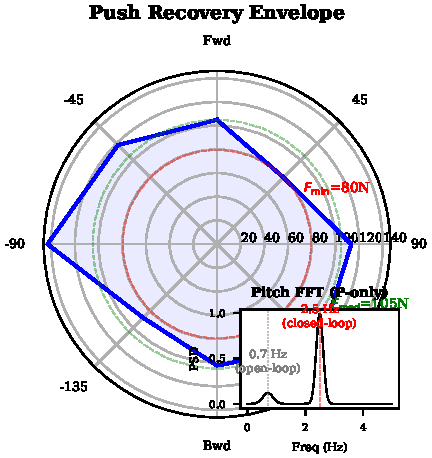
\includegraphics[width=\linewidth]{figures/polar_push_envelope.pdf}
    \caption{Omnidirectional push envelope of ACC. This is the \emph{same} run
    as row S1 of Table~\ref{tab:push_ablation}, not a separate measurement:
    \num{8} bearings, $N{=}\num{10}$ repetitions each, threshold located by
    binary search over \SIrange{10}{160}{N} to a \SI{5}{N} tolerance, so the
    plotted minimum is by construction the $F_{\min}$ of that row. Solid curve:
    per-bearing mean survivable push magnitude; shaded band: ${\pm}1$ standard
    deviation over the ten repetitions. The radial axis is linear in force and
    originates at \SI{0}{N}, so radial distance is proportional to margin.
    The envelope is strongly anisotropic, spanning
    \SIrange{82.3}{144.8}{N}---a $1.8{\times}$ ratio between the weakest and
    strongest bearing. The ordering is
    $-\SI{90}{\degree}\,(\SI{144.8}{N}) >
      \SI{135}{\degree}\,(\SI{132.2}{N}) >
      \SI{90}{\degree}\,(\SI{117.8}{N}) >
      -\SI{45}{\degree}\,(\SI{107.3}{N}) >
      \SI{180}{\degree}\,(\SI{100.7}{N}) >
      \SI{0}{\degree}\,(\SI{95.6}{N}) >
      -\SI{135}{\degree}\,(\SI{91.9}{N}) >
      \SI{45}{\degree}\,(\SI{82.3}{N})$.
    Two regularities are visible. First, the actuated axis is the strong one:
    bearings are applied in the world frame as
    $\mathbf{f}=F(\cos\theta,\sin\theta,0)$, so $\pm\SI{90}{\degree}$ are purely
    sagittal and $\SI{0}{\degree}/\SI{180}{\degree}$ purely lateral
    (Section~\ref{sec:standing}). The two sagittal bearings average \SI{131.3}{N}
    against \SI{98.2}{N} for the two lateral ones, a $1.34{\times}$ advantage.
    This is the expected asymmetry for a wheeled biped: sagittally the wheels
    accelerate the contact patch back under the CoM and convert the impulse into
    a controlled excursion, whereas laterally no actuator produces ground force
    at all and the only restoring authority is the static
    $w_{\text{track}}={\SI{0.278}{m}}$ track width plus hip-roll PD. We compare
    axis \emph{means} rather than ranks because the raw ordering is contaminated
    by the second regularity. Second, the envelope is
    measurably \emph{chiral}: $\SI{135}{\degree}$ survives \SI{40.3}{N} more than
    $-\SI{135}{\degree}$, and $-\SI{90}{\degree}$ \SI{27.0}{N} more than
    $\SI{90}{\degree}$. This is not sampling noise and not the plant, which is
    mirror-symmetric to numerical precision: it is the sign convention of the
    controller's antisymmetric hip-roll and hip-yaw channels, which leaves the
    closed loop $C_2$-equivariant but mirror-broken. The
    text traces it through the $\sin2\theta$ harmonic and closes the argument
    with two control experiments. $F_{\min}$ (red) is the bearing-wise minimum
    and is the figure of merit quoted throughout the paper, because it is the
    magnitude survived in \emph{every} direction; $F_{\max}$ (blue) is shown
    only to indicate the spread.}
    \label{fig:push_polar}
\end{figure}

\begin{figure}[pos=!htbp]
    \centering
    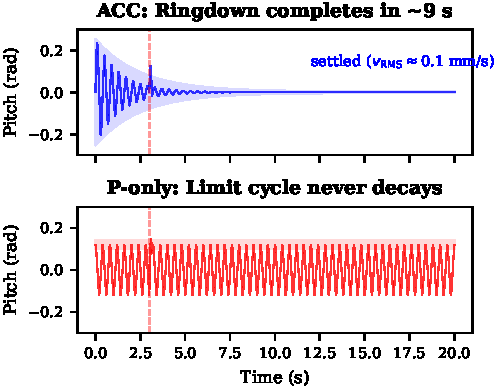
\includegraphics[width=\linewidth]{figures/ringdown_time_series.pdf}
    \caption{Post-push recovery (\SI{90}{N} lateral, world $+x$, at $t{=}\SI{3}{s}$). \textbf{Top:} attitude angles; stabilization within \SI{2}{s}. \textbf{Bottom:} planar CoM position, which separates the two axes cleanly. The lateral push couples through roll into a large \emph{sagittal} excursion (\SI{-251}{mm} peak); the anchor drives that axis back to $\SI{+1.37}{mm}$ of home and holds it there at \SI{0.018}{mm} SD over the final \SI{2}{s}---a \SI{99.5}{\percent} recovery. On the pushed lateral axis, which has no actuator authority (Section~\ref{sec:standing}), the \SI{200}{mm} peak excursion decays only to a permanent $\SI{+36.2}{mm}$ offset, \SI{18}{\percent} of the peak. The contrast between the two traces is the clearest single illustration of what the anchor does and where it does not act.}
    \label{fig:ringdown}
\end{figure}

\subsection{Flight Recovery and Terrain Adaptation}
\label{sec:flight_terrain_results}

ACC's two-channel assembly supports independent extensions without modifying the core anchor. Both extensions use the same \SI{400}{Nm/s} rate limit and \SI{100}{Hz} control rate.

\emph{Contact-loss recovery.}
ACC recovers to a settled stand from a \SI{100}{cm} free drop (10/10,
$24.0{\pm}1.2^\circ$ peak pitch after touchdown) and from a \SI{50}{cm} ledge
drive-off (10/10, $27.1{\pm}2.0^\circ$ peak landing pitch); the \SI{60}{cm} drop
and \SI{20}{cm} ledge are correspondingly milder (Table~\ref{tab:flight_ext}).
The two flight ablations, however, give a more nuanced picture than the
mechanism's design rationale suggests.

Removing the flight \emph{attitude} PD (the reaction-flywheel term
$2.0\theta + 0.5\dot\theta$, spin-down damping retained) is a real but modest
loss: peak pitch rises from $24.0$ to $\SI{27.8}{\degree}$ on the \SI{100}{cm}
drop with one fall in ten, and from $27.1$ to $\SI{31.6}{\degree}$ on the
\SI{50}{cm} ledge with no falls. Removing the airborne wheel-torque override
\emph{entirely}---so the ordinary wheel--inverted-pendulum (WIP) loop keeps
driving the wheels through flight---does not degrade either condition at all: it
\emph{lowers} peak pitch to $13.0{\pm}\SI{0.5}{\degree}$ (drop) and
$10.2{\pm}\SI{0.4}{\degree}$ (ledge) at 10/10 survival, because free wheels
driven by the pitch-feedback loop are themselves an effective reaction flywheel.
The override's benefit appears only at the upper end of the envelope: at
\SI{150}{cm} the two configurations survive equally (2/5 settled either way) but
the override holds peak pitch to $34.0{\pm}\SI{2.1}{\degree}$ against
$53.6{\pm}\SI{35.0}{\degree}$ without it---a \num{16}$\times$ reduction in
spread, with one uncontrolled trial exceeding \SI{90}{\degree}. At \SI{200}{cm}
both configurations fail. The flight override therefore \textbf{bounds
landing-attitude variance near the envelope limit} rather than enabling the
recovery; at the \SIrange{50}{100}{cm} scales reported here ACC's balance core
alone suffices.

\emph{Per-leg terrain adaptation.}
The success criterion here is traversal, not merely survival: a trial counts
only if the elevated wheel stays on the \SI{36}{cm}-wide slab for the whole
\SI{2}{m} straddle. A settling criterion alone cannot see this failure---a robot
that yaws off the side of the curb halfway along still lands on flat ground,
settles, and would score a pass on the tail criteria. Under the traversal
criterion, and with the straddle gating of Section~\ref{sec:terrain}, roll on the
one-wheel curb is $2.4{\pm}\SI{0.1}{\degree}$ (\SI{10}{cm}),
$2.9{\pm}\SI{0.2}{\degree}$ (\SI{15}{cm}) and $3.9{\pm}\SI{0.1}{\degree}$
(\SI{20}{cm}), \num{10}/\num{10} at every height.
The residual growth with step height is \emph{tracking} error, not a geometry
failure. Measured mid-straddle at \SI{20}{cm}, \eqref{eq:terrain_split} commands
a leg-length difference of \SI{0.193}{m} against the \SI{0.20}{m} step, leaving
$\varepsilon{=}\SI{7}{mm}$ unspanned, i.e.\ a predicted
$\arctan(\varepsilon/w_{\text{track}}){=}\SI{1.4}{\degree}$ of geometric roll, so
the remaining \SI{2.5}{\degree} is
servo error: in this deeply flexed configuration the compressed leg carries its
load at the shortest gravitational moment arm the PID gains were tuned for and
settles slightly below its target. The joint budget does tighten with height
without being the binding constraint at \SI{20}{cm}: the compressed leg's
commanded knee angle grows \SI{2.18}{rad}~(\SI{10}{cm}) $\rightarrow$
\SI{2.39}{rad}~(\SI{15}{cm}) $\rightarrow$ \SI{2.58}{rad}~(\SI{20}{cm}) against
a hard limit of \SI{2.70}{rad}, leaving \SI{0.12}{rad} (\SI{6.6}{\degree}) of
headroom.
Suppressing heading hold through the straddle instead---the behaviour before the
stability envelope's roll band was made split-dependent (Section~\ref{sec:terrain})---
leaves the mount transient undamped and the yaw error runs to the
\SI{0.30}{rad} command leash. Roll then measures $14.9{\pm}\SI{0.1}{\degree}$ at
\SI{20}{cm} ($N{=}10$) and the elevated wheel leaves the slab \SI{1.3}{m} into
the curb, verified at three seeds; the tight $\pm\SI{0.1}{\degree}$ std is a
deterministic runaway rather than genuinely low run-to-run variability.

The two component ablations are unambiguous. Replacing \texttt{split()} with a
symmetric posture (both legs commanded to the same height---the pre-adapter
behaviour) causes a fall at \emph{every} tested curb height, \num{0}/\num{10} in
all three cases: the torso rolls past \SI{60}{\degree} within \SI{0.8}{s} of
curb entry and the robot is on the ground by \SI{2.3}{s}. The straddle gating is
inert in this ablation, as it must be, since it is driven by the commanded
split. The height split is thus load-bearing for this task in a way the flight
override is not. Disabling the closed-loop leveling trim alone leaves the robot
upright on the \SI{10}{cm} curb ($4.5{\pm}\SI{2.3}{\degree}$, \num{10}/\num{10})
but collapses the \SI{15}{cm} curb to \num{1}/\num{10} and the \SI{20}{cm} curb
to \num{0}/\num{10} with five outright falls---the feedforward
height$\rightarrow$leg-length table alone does not span a step this large, and
the residual it leaves grows faster than the straddle allowance can absorb.

\emph{Oblique ledge descent: a straddle regime, not a height threshold.}
Driving off a ledge whose edge crosses the path at an angle $\phi$ releases the
two wheels a stagger interval $w_{\text{track}}\tan\phi/v$ apart, and only within
that interval can the leg split absorb the step. Instrumenting a
\SI{30}{\degree}, \SI{20}{cm} exit at \SI{0.7}{m/s} shows the window closing in
\SI{0.18}{s}: the split had commanded \SI{25}{mm} of differential leg travel
against the \SI{200}{mm} step when the trailing wheel lost contact, and the torso
absorbed the remainder, reaching $\SI{-33.1}{\degree}$ of roll against the
$\arctan(0.20/w_{\text{track}}){=}\SI{35.7}{\degree}$ that a wholly unspanned step
predicts. The legs were not at their travel limit when contact was lost
(\SI{99}{mm} of calibrated range unused), so the proximate failure is a race
rather than a saturation---though relieving it would not rescue this case,
because \SI{20}{cm} is itself unspannable at nominal stance (\SI{170}{\degree} of
knee flexion against the \SI{2.7}{rad} limit). The $\pm\SI{6}{cm}$ leveling trim
is unavailable throughout, since its gate requires \emph{both} wheels loaded.
Failure is consequently \emph{not} monotone in step height. Two regimes separate,
set by whether the leading wheel reaches the lower ground before the trailing
wheel releases---free fall over the step takes $\sqrt{2h/g}$, comparable to the
stagger interval at these heights. A shallow step lands the leading wheel while
the trailing wheel still bears on the platform, forcing the straddle the legs
cannot span; a deep step releases both wheels together and is handled by the
flight path of Section~\ref{sec:flight}. Widening the straddle regime requires knee
range rather than gains.

We calibrate the boundary at \num{192} trials---\num{12} heights
(\SIrange{12}{40}{cm}) ${\times}$ \num{8} independent initial conditions
${\times}$ two angles, \num{43}/\num{96} and \num{24}/\num{96} settled
(Table~\ref{tab:oblique_regime}). Both regimes are real and the dead band
between them is wide. At \SI{30}{\degree} the shallow window runs to
\SI{15}{cm} at \SI{100}{\percent}, degrades through \SI{17}{cm}
(\SI{75}{\percent}) and \SI{20}{cm} (\SI{25}{\percent}), and closes completely
over \SIrange{22}{27}{cm}; the deep regime then reopens from \SI{30}{cm} and
peaks at \SI{37}{cm} (\SI{75}{\percent}). At \SI{45}{\degree} the shallow window
is essentially gone---\SI{12}{\percent} at \SI{12}{cm}, zero from \SI{15}{cm} to
\SI{25}{cm}---and the deep regime opens later, at \SI{27}{cm}. That the window
shrinks with angle is what the stagger interval $w_{\text{track}}\tan\phi/v$
predicts, and it shrinks by roughly the right factor.
Two features are worth stating as measured rather than smoothed. Neither regime
reaches \SI{100}{\percent} at depth---the deep-regime maximum is
\SI{75}{\percent}, so a clean launch is a favorable initial condition and not a
guarantee. And the \SI{45}{\degree} column has a reproducible \num{0}/\num{8}
hole at \SI{32}{cm} sitting between \SI{50}{\percent} and \SI{62}{\percent}
neighbours, which the two-regime account does not predict. The boundary is
therefore calibrated as a success-probability field over launch height rather
than as a single threshold, and the \num{192}-trial grid resolves that field
directly.\footnote{\path{scripts/ramp_step_tests.py}
with \path{--seeds}; raw output \path{outputs/oblique_regime/diag30_fine.txt} and
\path{diag45_fine.txt}. Each seed perturbs the initial joint angles by
\SI{3}{mrad} and the root by \SI{1.5}{mm}, so the eight trials per cell sample
initial conditions on an otherwise deterministic course.}

\begin{table}[pos=!tbp]
\centering
\footnotesize
\caption{Oblique ledge descent: settle count out of \num{8} independent initial
conditions, at \SI{0.7}{m/s}. Two regimes separated by a dead band, not a height
threshold. Bold marks the dead band at each angle.}
\label{tab:oblique_regime}
\setlength{\tabcolsep}{5pt}\begin{tabular}{@{}lcc|lcc@{}}
\toprule
Step & \ang{30} & \ang{45} & Step & \ang{30} & \ang{45} \\
\midrule
\SI{12}{cm} & 8/8 & 1/8 & \SI{27}{cm} & \bfseries 0/8 & 5/8 \\
\SI{15}{cm} & 8/8 & \bfseries 0/8 & \SI{30}{cm} & 1/8 & 4/8 \\
\SI{17}{cm} & 6/8 & \bfseries 0/8 & \SI{32}{cm} & 3/8 & \bfseries 0/8 \\
\SI{20}{cm} & 2/8 & \bfseries 0/8 & \SI{35}{cm} & 4/8 & 5/8 \\
\SI{22}{cm} & \bfseries 0/8 & \bfseries 0/8 & \SI{37}{cm} & 6/8 & 6/8 \\
\SI{25}{cm} & \bfseries 0/8 & \bfseries 0/8 & \SI{40}{cm} & 5/8 & 3/8 \\
\addlinespace
\multicolumn{6}{@{}l}{Total: \ang{30} \num{43}/\num{96}; \ang{45} \num{24}/\num{96}} \\
\bottomrule
\end{tabular}
\vspace{2pt}\tabnote\noindent
Survival is the strict settle verdict of Table~\ref{tab:flight_ext}. The
\SI{32}{cm}/\ang{45} cell is a reproducible \num{0}/\num{8} between
\SI{50}{\percent} and \SI{62}{\percent} neighbours and is reported unsmoothed.
Produced by \path{scripts/ramp_step_tests.py --seeds}; raw output
\path{outputs/oblique_regime/diag\{30,45\}_fine.txt}.
\end{table}

\begin{table}[pos=!tbp]
\centering
\caption{Contact-loss recovery and per-leg terrain adaptation, with the
corresponding mechanism ablations. All at \SI{400}{Nm/s} rate limit,
\SI{100}{Hz} control. Survival is the \emph{strict settle} verdict (flat
pitch/roll window, tail height error ${\leq}\SI{12}{mm}$, residual speed
${\leq}\SI{0.05}{m/s}$), not merely staying upright.}
\label{tab:flight_ext}
\footnotesize
\setlength{\tabcolsep}{4pt}
\begin{tabular}{@{}>{\raggedright\arraybackslash}p{3.5cm}rrr@{}}
\toprule
\multicolumn{4}{c}{\textbf{Contact-Loss Recovery}} \\
\midrule
Scenario / ablation & $N$ & Peak Pitch ($^\circ$) & Settled \\
\addlinespace
Drop \SI{100}{cm}    & 10 & 24.0$\pm$1.2 & 10/10 \\
Drop \SI{60}{cm}     & 10 & 18.2$\pm$1.0 & 10/10 \\
Ledge \SI{50}{cm}    & 10 & 27.1$\pm$2.0 & 10/10 \\
Ledge \SI{20}{cm}    & 10 & 19.6$\pm$0.3 & 10/10 \\
\addlinespace[1pt]
$-$Attitude PD, drop \SI{100}{cm}\textsuperscript{a}   & 10 & 27.8$\pm$0.3 & 9/10 \\
$-$Attitude PD, ledge \SI{50}{cm}\textsuperscript{a}   & 10 & 31.6$\pm$2.2 & 10/10 \\
$-$Flight override, drop \SI{100}{cm}\textsuperscript{b} & 10 & 13.0$\pm$0.5 & 10/10 \\
$-$Flight override, ledge \SI{50}{cm}\textsuperscript{b} & 10 & 10.2$\pm$0.4 & 10/10 \\
\addlinespace[1pt]
Drop \SI{150}{cm} (envelope edge)      & 5 & 34.0$\pm$2.1 & 2/5 \\
$-$Flight override, drop \SI{150}{cm}\textsuperscript{b} & 5 & 53.6$\pm$35.0 & 2/5 \\
\addlinespace
\multicolumn{4}{c}{\textbf{Per-Leg Terrain (One-Wheel Curb, \SI{0.15}{m/s})}} \\
\addlinespace
Configuration & $N$ & Straddle Roll ($^\circ$) & Traversed \\
\addlinespace
Full adaptation, \SI{10}{cm}  & 10 & 2.4$\pm$0.1 & 10/10 \\
Full adaptation, \SI{15}{cm}  & 10 & 2.9$\pm$0.2 & 10/10 \\
Full adaptation, \SI{20}{cm}  & 10 & 3.9$\pm$0.1 & 10/10 \\
\addlinespace[1pt]
$-$Straddle gating, \SI{20}{cm}\textsuperscript{c} & 10 & 14.9$\pm$0.1 & 0/10 \\
\addlinespace[1pt]
$-$Leveling trim, \SI{10}{cm}\textsuperscript{d} & 10 & 4.5$\pm$2.3 & 10/10 \\
$-$Leveling trim, \SI{15}{cm}\textsuperscript{d} & 10 & 10.7 & 1/10 \\
$-$Leveling trim, \SI{20}{cm}\textsuperscript{d} & 10 & \multicolumn{1}{c}{fall} & 0/10 \\
\addlinespace[1pt]
$-$Height split, \SI{10}{cm}\textsuperscript{e} & 10 & \multicolumn{1}{c}{fall} & 0/10 \\
$-$Height split, \SI{15}{cm}\textsuperscript{e} & 10 & \multicolumn{1}{c}{fall} & 0/10 \\
$-$Height split, \SI{20}{cm}\textsuperscript{e} & 10 & \multicolumn{1}{c}{fall} & 0/10 \\
\bottomrule
\end{tabular}
\vspace{2pt}\tabnote\noindent
$\pm$std over $N$ trials with randomized ICs ($\pm\SI{0.003}{rad}$ joint,
$\pm\SI{1.5}{mm}$ CoM). Drop metric: peak $|\theta|$ from touchdown onward;
ledge metric: peak $|\theta|$ through landing; curb metric: max $|\phi|$ while
straddling the curb top, over traversing trials only. ``Traversed'' requires the
elevated wheel to stay on the \SI{36}{cm} slab for the whole \SI{2}{m} straddle,
not merely to settle afterwards.
\textsuperscript{a}Reaction-flywheel attitude PD zeroed; airborne spin-down damping retained.
\textsuperscript{b}Entire airborne wheel-torque override bypassed---the ordinary WIP loop drives the wheels through flight.
\textsuperscript{c}Split-dependent straddle roll band and settled-terrain relaxation removed, i.e.\ heading hold suppressed for the whole crossing; the robot yaws off the slab \SI{1.3}{m} in but lands upright on flat ground and settles, which is why a settling-only criterion scored this configuration 10/10.
\textsuperscript{d}Closed-loop leveling integrator disabled; per-leg height split retained. At \SI{15}{cm} the single traversing trial gives no std; at \SI{20}{cm} five of ten fall outright.
\textsuperscript{e}\texttt{split()} forced to a symmetric posture (both legs at the same commanded height), i.e.\ pre-adapter behaviour; roll diverges past \SI{60}{\degree} within \SI{0.8}{s} of curb entry, so no straddle-roll statistic exists.
\tabnote\noindent
Produced by \path{scripts/collect_flight_terrain_n10.py}; raw output
\path{outputs/flight_terrain_n10/results.json}.
\end{table}

The gate structure isolates each extension to its physical regime without
re-tuning the anchor, and both extensions cost three lines of controller code
each. Their measured \emph{necessity}, however, differs sharply: the per-leg
height split is required for the curb task at every tested height, whereas the
flight override is a variance-bounding refinement that only pays at the top of
the drop envelope.

\begin{figure}[pos=!htbp]
    \centering
    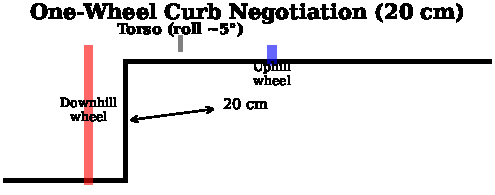
\includegraphics[width=\linewidth]{figures/curb_straddle.pdf}
    \caption{One-wheel curb (\SI{20}{cm}). With the per-leg height split and the
    straddle gating of Section~\ref{sec:terrain}: $3.9{\pm}0.1^\circ$ straddle roll,
    10/10 traversed. With a symmetric posture (split removed): the curb-side leg
    cannot fold far enough, roll diverges past \SI{60}{\degree} within
    \SI{0.8}{s} of curb entry, 0/10.}
    \label{fig:curb}
\end{figure}

\subsection{Comparison with Classical Baselines and a Preliminary RL Reference}
\label{sec:baselines}

To establish that ACC is not merely a tuned linear controller, we compare six classical baselines---four 4-state TWIP variants (LQR, LQR+AW, LQR-DT, PI+AW) and two 6-state coupled variants (servo and direct-torque)---together with a preliminary model-free PPO run reported as a reference point rather than as a seventh baseline (all share identical environment setups):

\begin{enumerate}
\item \textbf{LQR}---4-state TWIP~\cite{grasser2002joe,pathak2005wip} with decoupled roll/yaw PD through a PID servo layer ($\sim$\SI{0.25}{s} lag).
\item \textbf{LQR + Integral AW}---Same as (1) plus pitch-error integral with conditional AW (clamped $\pm\SI{3.0}{rad/s}$).
\item \textbf{LQR (Direct Torque)}---Re-optimized for direct-torque plant ($\tau_s{=}0$, $k_{p,\text{roll}}{=}55.0$), outputting torques directly.
\item \textbf{Coupled 6-State 3D LQR}---Extends (1) with roll states $(\phi,\dot{\phi})$.
\item \textbf{PI + AW (Direct Torque)}---DT-LQR $+$ integral AW on fwd.\ position (conditional, $\pm\SI{15}{cm}$ gate); same leg/roll/yaw as DT-LQR.
\item \textbf{PPO reference (preliminary)}---Model-free policy trained from scratch for \num{5.4}M environment steps in \texttt{BalanceEnv}: single seed, no domain randomization, no hyperparameter search. Included as a difficulty probe, not as a tuned RL baseline (Limitation~4).
\item \textbf{Coupled 6-State LQR (Direct Torque)}---Same 6-state model as (4) but outputs direct torques (bypassing PID servo, $\sim$\SI{0.25}{s} lag removed). Gains re-derived for the direct-torque plant ($K_{\text{pitch}}{=}113$, $K_{\text{roll}}{=}58$\,Nm/rad); leg posture via PD position control.
\end{enumerate}

Direct-torque LQR removes the servo path, eliminating both the PID gains and the measured actuation lag. PI+AW adds integral anti-windup on forward position to DT-LQR---the standard engineering fix for a DC position bias, with windup protection. The anti-windup logic is verified independently by \texttt{scripts/validate\_lqr\_aw.py}. The PPO run serves a different purpose from the six classical controllers. It is included not to benchmark the state of the art in reinforcement learning, but to characterize how hard unaided model-free search is on the coupled pitch--height state space of a 10-DOF wheeled biped, and thereby to make explicit the value of the structured gate design ACC supplies in its place. Every gain used for the six classical baselines is listed in Table~\ref{tab:baseline_gains}; we give them in full because the central claim of this subsection is a \emph{negative} one---that no member of this family stands---and a negative result is only as strong as the tuning behind it.

\begin{table}[pos=!tbp]
\centering
\footnotesize
\caption{Baseline gain derivation. All weights follow Bryson's rule~\cite{bryson1975optimal}; see the note below the table.}
\label{tab:baseline_gains}
\setlength{\tabcolsep}{4pt}
\begin{tabular}{@{}>{\raggedright\arraybackslash}p{1.75cm}>{\raggedright\arraybackslash}p{6.15cm}@{}}
\toprule
Controller & Gains and derivation \\
\midrule
LQR (4-state) & $Q{=}\operatorname{diag}(10,2,3,0.3)$, $R{=}0.8$; roll and yaw closed by decoupled PD through the PID servo layer \\
\addlinespace[2pt]
LQR $+$ AW & as above, plus a pitch-error integral with conditional anti-windup, clamped to $\pm\SI{3.0}{rad/s}$ \\
\addlinespace[2pt]
LQR, DT & 4-state gains re-optimized for the zero-lag plant: $\tau_s{=}0$, $k_{p,\text{roll}}{=}55.0$ \\
\addlinespace[2pt]
6-state LQR & $Q{=}\operatorname{diag}(10,2,3,0.5,3,0.3)$, $R{=}\operatorname{diag}(0.8,1.0)$, derived in continuous time and shared by the servo and DT variants \\
\addlinespace[2pt]
6-state LQR, DT & state feedback re-solved for the zero-lag plant: $K_{\text{pitch}}{=}113$, $K_{\text{roll}}{=}\SI{58}{Nm/rad}$ (see Limitation~4) \\
\addlinespace[2pt]
PI $+$ AW, DT & DT-LQR gains plus an integral on forward position: $k_{i,\text{pos}}{=}\SI{8.0}{rad/s/(m{\cdot}s)}$, clamp $\pm\SI{5.0}{rad/s}$, conditional gate $\pm\SI{15}{cm}$ \\
\addlinespace
PID servo layer & $k_p{=}[55,40,70,70,4]$, $k_d{=}[3,2,4,4,0]$, $k_i{=}[0.8,0.4,1,1,0.1]$, ordered (hip roll, hip yaw, hip pitch, knee, wheel) \\
\addlinespace[2pt]
Servo lag & \SI{0.25}{s}, measured as the wheel-velocity \SI{90}{\percent} rise time ($\approx\num{25}$ steps at \SI{100}{Hz}) \\
\bottomrule
\end{tabular}
\vspace{2pt}\tabnote\noindent\footnotesize
Bryson's rule throughout ($Q_{ii}{=}1/x_{i,\max}^{2}$, $R{=}1/u_{\max}^{2}$); the \num{46}-configuration retuning sweep described in the text confirmed that no retuning within these ranges changes the outcome. The 4-state model is (pitch, pitch-rate, forward velocity, forward position); the 6-state model adds (roll, roll-rate). ``DT'' denotes direct torque, i.e.\ the PID servo path removed and $\tau_s{=}0$.
\end{table}

\begin{table}[pos=!tbp]
\centering
\footnotesize
\caption{Classical baselines and the preliminary PPO reference vs.\ ACC, clean sensors. All rows at \SI{100}{Hz} control except the PPO reference, which is reported at the \SI{50}{Hz} rate its policy was trained at. Parenthesised $N$ is the episode count. See the note below the table.}
\label{tab:lqr_baselines}
\setlength{\tabcolsep}{4pt}
\begin{tabular}{@{}l S[table-format=2.2] S[table-format=1.3] S[table-format=2.2] S[table-format=3.1] S[table-format=2.2]@{}}
\toprule
Configuration & {Surv.} & {$\theta_{\text{RMS}}$} & {$\phi_{\text{RMS}}$} & {$H_{\text{RMS}}$} & {$\tau_{\text{RMS}}$} \\
& {(s)} & {(\si{\degree})} & {(\si{\degree})} & {(mm)} & {(Nm)} \\
\midrule
LQR, TWIP ($N{=}20$)         & 0.32 & 0.006 & 24.2 & 205.8 & 21.99 \\
LQR $+$ AW ($N{=}20$)        & 0.32 & 0.006 & 24.2 & 205.8 & 21.99 \\
LQR, DT (re-opt.) ($N{=}20$) & 0.60 & 0.033 & 27.5 & 119.2 & 8.76 \\
6-St.\ LQR ($N{=}20$)        & 0.32 & 0.006 & 24.2 & 205.8 & 21.99 \\
PI $+$ AW, DT ($N{=}20$)     & 0.52 & 0.181 & 26.1 & 171.3 & 10.42 \\
6-St.\ LQR, DT ($N{=}20$)    & 0.16 & 0.001 & 21.2 & 128.5 & 14.44 \\
PPO ref.\ (\SI{50}{Hz}) ($N{=}20$)& 3.20 & 4.82  & 3.15 & 54.2  & 18.40 \\
\addlinespace
\textbf{ACC} ($N{=}10$)      & \bfseries 20.00 & \bfseries 0.060 & \bfseries 0.010 & \bfseries 0.18 & \bfseries 3.28 \\
\bottomrule
\end{tabular}
\vspace{3pt}\tabnote\noindent\footnotesize
LQR / LQR+AW / 6-St.\ use the PID servo; LQR (DT), PI+AW (DT) and 6-St.\ (DT) command torque directly; PPO is a 5.4M-step model-free run (preliminary, single seed, no domain randomization), reported as a reference point rather than a tuned RL baseline. The identical LQR / LQR+AW / 6-St.\ rows arise because all three command through the same PID servo path, whose response dominates before the gain differential between them can act; the coincidence holds at both control rates (Table~\ref{tab:rate_matched}).\tabnote\noindent
Between-episode standard deviations (omitted above for legibility): survival time is
deterministic on all six classical rows ($\pm\SI{0.00}{s}$ at $N{=}20$, seeds $\{0,42,123\}$);
PPO: $\pm0.85$, $\pm0.91$, $\pm0.45$, $\pm8.3$, $\pm2.1$;
ACC: $\pm0.00$, $\pm0.006$, $\pm0.001$, $\pm0.02$, $\pm0.00$.
Per-metric between-episode dispersions for the classical rows are not retained in the
rate-matched output (\path{outputs/rate_matched_baselines/results.json}), which stores
episode-aggregated values.
\vspace{2pt}\tabnote\noindent All LQR and PI+AW variants fall within \SI{0.60}{s} (\SI{100}{\percent}); the 6-St.\ DT variant falls deterministically at \SI{0.16}{s} (zero trial-to-trial variance), confirming that removing the servo path with gains derived from a simplified model does not rescue stability. PI+AW (DT-LQR $+$ integral AW on fwd.\ position) does not improve on DT-LQR at this rate---it is \SI{0.08}{s} worse---because the integral cannot accumulate usefully before the roll-induced fall. The PPO reference achieves partial standing but suffers \SI{85}{\percent} falls over multi-height transitions ($H_{\text{RMS}}{=}\SI{54.2}{mm}$). $N{=}20$ throughout; classical rows from \path{outputs/rate_matched_baselines/results.json}.
\end{table}

Table~\ref{tab:lqr_baselines} reports the comparison.
All six classical baselines---four derived from the 4-state TWIP model (LQR, LQR+AW, LQR-DT, PI+AW) and two 6-state coupled variants (servo, direct-torque)---fall within \SI{0.60}{s}. Removing the PID servo path (4-state DT-LQR: $\tau_s{=}0$, $k_{p,\text{roll}}{=}55.0$, no integral) cuts torque by \num{2.5}$\times$ (\SI{21.99}{Nm} $\rightarrow$ \SI{8.76}{Nm}) and nearly doubles survival (\SI{0.32}{s} $\rightarrow$ \SI{0.60}{s}), but \emph{worsens} roll ($\phi_{\text{RMS}}{=}\SI{27.5}{\degree}$ vs.\ \SI{24.2}{\degree}): the recovered authority is spent in the sagittal plane the model describes, not in the lateral one that ends the episode. Adding a forward-position integral (PI+AW: $k_{i,\text{pos}}{=}8.0$, conditional $\pm\SI{15}{cm}$ gate) gives back \SI{0.08}{s} of that gain rather than adding to it---the integral cannot accumulate usefully before the roll-induced fall---confirming the 4-state TWIP model is structurally insufficient for this articulated-leg platform.
The preliminary PPO reference (5.4M steps, single seed) sustains single-height standing longer (\SI{3.20}{s}) but exhibits an \SI{85}{\percent} fall rate across multi-height command transitions (\SI{54.2}{mm} height error). Read as a difficulty probe rather than a comparison, this is the observation the structured prior is meant to address: unaided search spends its budget rediscovering the pitch--height coupling that the posture map and the gate schedule encode directly.
ACC achieves $0.060{\pm}0.006^\circ$ pitch RMS, $0.010{\pm}0.001^\circ$ roll RMS, $0.18{\pm}0.02$\,mm CoM Z, and $3.28{\pm}0.00$\,Nm torque RMS ($N{=}10$).
A \textbf{46-configuration} sweep (dimensions as given in Table~\ref{tab:baseline_gains}; script \path{scripts/sweep_lqr_roll_gains.py}) confirmed all tested LQR variants fail (\SI{100}{\percent}); a 6-state coupled LQR with direct torque actuation, removing the PID servo path, also fails---indicating platform complexity, not servo lag alone, is the dominant factor (see Limitation~4).
Neither servo-lag removal nor preliminary PPO training (5.4M steps, single seed) resolved the height-adaptive posture trade-off in our experiments; whether a fully converged PPO policy closes this gap is not tested here.

\subsubsection{Both control rates give the same outcome}
\label{sec:rate_matched}

Table~\ref{tab:lqr_baselines} reports every classical baseline at ACC's \SI{100}{Hz}, so the headline comparison carries no control-bandwidth differential. Those gains were tuned for a \SI{50}{Hz} loop, however, and a reader is entitled to ask whether running them off their design rate is what produces the gap. Table~\ref{tab:rate_matched} answers that by giving both rates side by side.

\begin{table}[pos=!tbp]
\centering
\footnotesize
\caption{Every classical controller at both control rates: its own \SI{50}{Hz} design rate and ACC's \SI{100}{Hz} (the rate used in Table~\ref{tab:lqr_baselines}). Physics is \SI{500}{Hz} throughout; only the substeps per control step change. See the note below the table.}
\label{tab:rate_matched}
\setlength{\tabcolsep}{2.2pt}
\begin{tabular}{@{}l S[table-format=1.2] S[table-format=2.2] S[table-format=2.2] S[table-format=2.2] S[table-format=3.1] S[table-format=3.1]@{}}
\toprule
& \multicolumn{2}{c}{Surv.\ (s)} & \multicolumn{2}{c}{$\phi_{\text{RMS}}$ (\si{\degree})} & \multicolumn{2}{c}{$H_{\text{RMS}}$ (mm)} \\
\cmidrule(lr){2-3}\cmidrule(lr){4-5}\cmidrule(lr){6-7}
Configuration & {\SI{50}{Hz}} & {\SI{100}{Hz}} & {\SI{50}{Hz}} & {\SI{100}{Hz}} & {\SI{50}{Hz}} & {\SI{100}{Hz}} \\
\midrule
LQR, TWIP        & 0.52 & 0.32 & 24.21 & 24.21 & 370.6 & 205.8 \\
LQR $+$ AW       & 0.52 & 0.32 & 24.19 & 24.21 & 370.7 & 205.8 \\
LQR, DT          & 0.72 & 0.60 & 21.22 & 27.48 & 135.0 & 119.2 \\
6-St.\ LQR       & 0.52 & 0.32 & 24.20 & 24.21 & 370.6 & 205.8 \\
PI $+$ AW, DT    & 0.72 & 0.52 & 21.22 & 26.14 & 135.0 & 171.3 \\
6-St.\ LQR, DT   & 0.16 & 0.16 & 21.05 & 21.19 & 117.2 & 128.5 \\
\addlinespace
\textbf{ACC}     & {---} & \bfseries 20.00 & {---} & \bfseries 0.010 & {---} & \bfseries 0.18 \\
\bottomrule
\end{tabular}
\vspace{3pt}\tabnote\noindent\footnotesize
\textbf{Protocol.} $N{=}20$ episodes per cell, seeds $\{0,42,123\}$, nominal scenario, clean sensors, \SI{0}{ms} actuator delay. Episode length is held fixed in \emph{seconds}, not steps: \num{1000} steps at \SI{50}{Hz} and \num{2000} steps at \SI{100}{Hz} both cover \SI{20}{s}. The LQR feedback gains are continuous-time and therefore rate-independent; the rate change affects only the substep count, the drift and integral accumulators, the torque rate limiter, and (for the FD-linearized variant) the linearization step.\tabnote\noindent
\textbf{Outcome.} Fall rate is \SI{100}{\percent} in all twelve baseline cells. The \SI{100}{Hz} columns are the ones carried into Table~\ref{tab:lqr_baselines}; the \SI{50}{Hz} columns come from the same script and the same episodes, so the two rates differ only by the intended change. ACC is shown at \SI{100}{Hz} only; the \SI{50}{Hz} ACC run is analysed as a negative result in Limitation~2 and is not a usable row.
\tabnote\noindent Produced by \path{scripts/collect_rate_matched_baselines.py} (\texttt{--control-hz} flag added to \path{scripts/eval_balance.py}); raw output \path{outputs/rate_matched_baselines/results.json}.
\end{table}

Doubling the baselines' control rate does not rescue any of them. Fall rate remains \SI{100}{\percent} in every cell, and survival time does not improve for a single variant---it \emph{shortens} for five of six (LQR: \SI{0.52}{s}$\rightarrow$\SI{0.32}{s}; LQR-DT: \SI{0.72}{s}$\rightarrow$\SI{0.60}{s}; PI+AW: \SI{0.72}{s}$\rightarrow$\SI{0.52}{s}) and is unchanged for the sixth. The diagnostic quantity is roll: $\phi_{\text{RMS}}$ is \SI{24.21}{\degree} at both rates for the three servo variants, and rises from \SI{21.22}{\degree} to \SI{27.48}{\degree} for LQR-DT. Faster sampling improves the quantities the controller actually regulates---pitch RMS falls by roughly $6{\times}$ for the servo variants (\SI{0.037}{\degree}$\rightarrow$\SI{0.006}{\degree}) and $\tau_{\text{RMS}}$ drops from \SI{92.1}{Nm} to \SI{22.0}{Nm}---while leaving the lateral divergence that terminates the episode untouched. This is the signature of a model-structure deficit rather than a bandwidth deficit: the 4-state TWIP model carries no lateral state at all, and the 6-state coupled variant carries roll but linearizes it about a single operating point, so no sampling rate supplies the missing dynamics. Reporting the baselines at \SI{100}{Hz} in Table~\ref{tab:lqr_baselines} is the rate-matched choice, and it is deliberately not the flattering one for them: five of the six survive \emph{longer} at \SI{50}{Hz}. Both rates are given here so that the comparison can be read either way, and the fall rate is \SI{100}{\percent} in all twelve cells.

The converse experiment---running ACC at \SI{50}{Hz}---is a negative result: the controller does not survive the rate change, and it is recorded as a limitation (Section~\ref{sec:discussion}, Limitation~2) rather than as a rate-independence claim. What Table~\ref{tab:rate_matched} establishes is the direction that matters for the comparison: the classical baselines fail both at the rate for which they were designed and at ACC's rate.

\subsubsection{A full-state LQR designed on the plant itself}
\label{sec:full_state_lqr}

All six baselines above are designed on a reduced model, so their failure is open to the obvious objection that the model, not the method, is what fails. The control experiment that settles this is a linear-quadratic regulator derived from the plant directly: a damped Gauss--Newton solve for a true static equilibrium $(\mathbf{x}^\ast,\mathbf{u}^\ast)$ at the commanded height, central differences on the whole held-input control step of the complete 16-DOF, 10-actuator MuJoCo model for the transition Jacobians, removal of the two cyclic wheel-angle states, and a discrete-time Riccati solve on the remaining \num{30}. Torque is emitted under the same \SI{400}{Nm/s} rate limit as every other row, and Bryson's rule~\cite{bryson1975optimal} fixes $\mathbf{Q}$ and $\mathbf{R}$ from physical maximum deviations, leaving one knob---a uniform control weight $r$---swept over six decades rather than tuned. The design is sound on every diagnostic that bears on it: at the \SI{0.65}{m} equilibrium the residual unbalanced force is \SI{0.428}{N} against \SI{79.46}{N} of body weight (\SI{0.54}{\percent}), the reduced $\mathbf{A}$ has full rank \num{30} and is PBH-stabilizable, the Riccati relative residual is ${\sim}10^{-14}$, and the designed closed loop has $\max|\lambda|{=}0.9911$. The one figure that invites a disqualifying reading, $\kappa(\mathbf{A}){\approx}10^{10}$, does not support it: it is a \SI{50}{Hz} artifact ($2.6{\times}10^{7}$ at \SI{100}{Hz}) traceable to a ${\sim}10^{-9}$ \emph{smallest} singular value---strongly \emph{contracting} contact modes---and it obstructs neither the Riccati solve nor the resulting feedback. Whatever limits this controller, it is not the linearization.

What the sweep shows instead is a slow divergence that a short horizon hides. Over \SI{20}{s} the design looks successful: at $h{=}\SI{0.65}{m}$, $r{=}1000$ gives \SI{0}{\percent} falls with \SI{11.0}{mm} height RMSE and \SI{0.12}{\degree} pitch RMS. At \SI{60}{s} every configuration tested falls in \SI{100}{\percent} of episodes, at \SIrange{22.2}{57.0}{s}, with planar drift growing monotonically to \SIrange{0.43}{0.63}{m}---that drift, not attitude, is what ends them. Nor does one weight cover the band: $r{=}100$ stands \SI{20}{s} at \SI{0.60}{m} and \SI{0.69}{m} but falls at \SI{0.65}{m}, $r{=}1000$ does the reverse, and under uniformly random height commands in \SIrange{0.40}{0.70}{m} the fall rate runs \SIrange{45}{80}{\percent} across the three usable weights. At the baselines' own \SI{50}{Hz} rate every weight falls inside \SI{20}{s}. Push separates it from ACC outright: \SI{100}{\percent} falls under the standard \SI{50}{N} impulse, and a maximum recoverable push of \SIrange{10.0}{20.2}{N} against ACC's $F_{\min}{=}\SI{82}{N}$. The reading is therefore not that the plant defeats linearization---it does not---but that full-state optimal linear feedback about a single equilibrium buys roughly two orders of magnitude of survival over the reduced-order designs (\SIrange{0.16}{0.60}{s} $\rightarrow$ \SIrange{22}{57}{s}) and still does not close the problem: it diverges slowly rather than quickly, holds one height at a time rather than the band, and has essentially no push envelope. Two of those three are exactly what the anchor integral and the gate schedule are for, which is why the full-state design is reported as a control experiment rather than promoted into Table~\ref{tab:lqr_baselines}---at the \SI{20}{s} horizon used for every other row it would read as a partial success, and that reading is an artifact of the horizon.\footnote{$N{=}20$ episodes $\times$ seeds $\{0,42,123\}$ per configuration at \SI{100}{Hz}; between-episode SD is \SI{0.00}{s} on time-to-fall, and weights $r{<}100$ fall within \SI{1.4}{s}. Produced by \path{scripts/eval_balance.py --controller baseline_full_lqr}; per-configuration results and the design diagnostics are in \path{outputs/fullstate_lqr_corrected/}, whose \path{README.md} maps each row to its run.}

\subsubsection{Sensitivity of the coupled model's empirical roll coupling}
\label{sec:b_roll_hip}

The two 6-state coupled baselines close their roll channel with a constant $b_{r,h}$ (hip-roll angle to roll acceleration) that the planar pendulum model does not supply in closed form; it was set empirically to $-5.0$. Since the negative result of this subsection rests on those rows, that constant is swept rather than assumed: nine values from \num{-0.5} to \num{-40} (an \num{80}$\times$ range spanning both sides of the nominal), gains re-derived through the same Riccati solve at each value, both variants, $N{=}20$ episodes $\times$ seeds $\{0,42,123\}$ at \SI{100}{Hz}.

The outcome does not move. The servo variant falls in \SI{100}{\percent} of episodes at \SI{0.320}{s} for every value, with roll RMS between \SI{24.209}{\degree} and \SI{24.224}{\degree} (a spread of \SI{0.06}{\percent}); the direct-torque variant falls at \SI{0.160}{s} for every value, with roll RMS \SIrange{21.186}{21.187}{\degree}. This is invariance to the parameter, not insensitivity of the metric: the re-derived roll gain varies \num{32}$\times$ across the sweep for the servo path (\SIrange{2.24}{72.71}{}) and \num{8}$\times$ for the torque path. The mechanism is saturation. The roll-channel command reaches its ceiling---the $\pm\SI{0.7}{rad}$ hip-roll joint limit for the servo path---at a roll excursion of \SIrange{0.55}{17.87}{\degree} depending on $b_{r,h}$, while the roll excursion actually observed before the fall has an RMS of \SI{24.2}{\degree}. The channel is therefore commanded against its limit throughout the episode at every value in the sweep, and the gain that computed the command cannot matter. Raw output: \path{outputs/b_roll_hip_sweep/results_100hz.json} (\path{scripts/sweep_b_roll_hip.py}).


% ============================================================
\subsection{Whole-Body Control Baselines}
\label{sec:wbc}
% ============================================================

To address whether a tuned whole-body controller (WBC) could match ACC, we evaluated two WBC configurations that were developed and subsequently discarded during controller development:
\textbf{(W1)}~a task-priority quadratic-program (QP) WBC---minimizing COM height error, torso orientation error, posture damping, and wheel regularization subject to full-body dynamics and contact constraints---used as the \emph{primary} balance controller; and
\textbf{(W2)}~the same WBC blended as an \emph{assist} on top of ACC via $\boldsymbol{\tau}_{\text{assist}} = \boldsymbol{\tau}_{\text{ACC}} + \alpha\!\cdot\!(\boldsymbol{\tau}_{\text{wbc}} - \boldsymbol{\tau}_{\text{ACC}})$, evaluated both with the per-joint authority gate active and with it disabled.
Both were evaluated under identical cloned simulation conditions (three-arm counterfactual: ACC baseline, WBC-only, ACC$+$WBC assist; 225 scenarios spanning fixed-height balance, height transitions, and push recovery at \SIrange{20}{120}{N}; \num{481000} control steps; ACC profile \texttt{K2\_JAX\_DEDICATED\_DEFAULT\_V3}; no gain retuning).
So that the comparison is not a verdict on our own implementation, the WBC was verified against executable references before evaluation---its analytic contact Jacobian against MuJoCo's \texttt{mj\_jac}, its task stack against each of four independently selectable weightings, and its height reference against the CoM-$z$ convention of Section~\ref{sec:height_convention} (Appendix~\ref{sec:wbc_supp}, Table~\ref{tab:wbc_verification}). Every number below comes from that verified implementation.

\medskip\noindent\textbf{W1 (WBC as primary controller).}
The standalone QP-WBC falls in \textbf{225 of 225} scenarios; ACC falls in \textbf{none}.
It holds the robot upright for \SI{0.570}{s} (SD \SI{0.001}{s}) and spends \SI{97.3}{\percent} of every episode in a fallen state (\num{468179} of \num{481000} control steps).
The failure is \emph{lateral}: roll RMS is \SI{93.45}{\degree} against ACC's \SI{3.71}{\degree} ($\num{25.2}\times$) and peaks at \SI{103.9}{\degree}---past horizontal---while pitch RMS is only \SI{2.33}{\degree} against \SI{0.52}{\degree} ($\num{4.5}\times$).
Base height collapses from \SI{0.540}{m} to \SI{0.091}{m}.
The fallen fraction is uniform across all five scenario suites (\SIrange{97.2}{97.4}{\percent}), so the collapse is not specific to pushes or to commanded height changes.

\medskip\noindent\textbf{The failure is invariant to implementation quality.}
Solver quality is not what decides the outcome, and a control experiment isolates it: a degraded build of the same controller, whose QP returns a usable solution on only \SI{85.85}{\percent} of steps, falls at \SI{0.52}{s}, while the verified build---\SI{99.99}{\percent} solved (\num{480950} of \num{481000} steps), commanded torque RMS \SI{0.96}{Nm} and max \SI{4.33}{Nm}---falls at \SI{0.570}{s}.
A \num{14}-point improvement in solve rate buys \SI{50}{ms} of upright time against a \SI{0.570}{s} lifetime.
Nor is the failure an artifact of one task weighting: re-running the WBC-only arm at four task-weight modes over an identical scenario set (Table~\ref{tab:wbc_taskweight}) moves the fallen fraction by \num{0.1} percentage points and upright time by \SI{0.03}{s}.
The best mode, \texttt{torso\_priority}, improves pitch RMS by \SI{40}{\percent} but \emph{worsens} roll---within a single SO(3) orientation task carrying equal roll and pitch gains, the QP trades one axis against the other rather than fixing both.

\medskip\noindent\textbf{Mechanism.}
The WBC's posture task is a velocity damper, not a position tracker.
Its reference $\mathbf{q}_{\text{ref}}$ is rebuilt from the currently measured joint vector at every control step, so $\mathbf{q}-\mathbf{q}_{\text{ref}} \equiv \mathbf{0}$ identically and the task collapses to $-k_{d,\text{posture}}\dot{\mathbf{q}}$ with $k_{d,\text{posture}}{=}2.0$.
It can slow a postural drift but cannot reverse one.
Combined with the absence of gravity-compensation feedforward, nothing in the task stack restores the legs once a lateral excursion begins---which is why the collapse is lateral, why it is insensitive to the task weighting, and why solver quality does not delay it.
Critically, this is not a matter of tuning or of implementation: the WBC lacks the \emph{regime-gating} that ACC's proximity-gated anchor provides.
A WBC distributes torque optimally for a fixed task set---it cannot express qualitatively distinct physical regimes (quiet stance, push ringdown, large excursion) as distinct control modes.
The precision--recovery trade-off ACC resolves through spatial gating and asymmetric temporal envelope-following is not expressible as a task-priority QP objective; even an ideally implemented WBC would lack the structured prior that gates the anchor integral, and would therefore face the same global-integral windup that our ablation S4 (no proximity gate, Table~\ref{tab:push_ablation}) confirms is fatal for sub-millimeter precision.

\medskip\noindent\textbf{W2 (WBC as assist on ACC).}
We ran the assist in both of its available configurations, which together constitute a gate ablation (Table~\ref{tab:wbc_three_arm}).

\emph{Gate disabled} ($\alpha{=}0.25$ fixed, per-joint authority capped at \SI{20}{\percent} of the ACC torque; this is the configuration behind the 225-scenario campaign). The QP solved on \SI{100.0000}{\percent} of steps with zero fail-closed events, so WBC torque entered the blend unconditionally. The assist arm never falls---ACC carries it---but it degrades ACC on every metric except one: pitch RMS \SI{1.295}{\degree} vs.\ \SI{0.520}{\degree} ($\num{2.5}\times$), yaw drift \SI{12.56}{\degree} vs.\ \SI{6.69}{\degree} ($\num{1.9}\times$), planar drift \SI{0.199}{m} vs.\ \SI{0.099}{m} ($\num{2.0}\times$), height RMS \SI{0.518}{m} vs.\ \SI{0.540}{m}, and torque RMS \SI{3.67}{Nm} vs.\ \SI{3.18}{Nm}.

\emph{Gate enabled} (per-joint authority $\alpha_{j} = \alpha_{\max}\!\cdot\!g_{\text{stability}}\!\cdot\!g_{\text{height}}\!\cdot\!g_{\text{push}}\!\cdot\!g_{\text{divergence}}\!\cdot\!A_j\!\cdot\!K_{\text{role},j}$, $\alpha_{\max}{=}0.25$). We instrumented the gate to record $\alpha$ and every factor at every control step. On the one height variant where the gate opens at all, the admitted authority is $\bar\alpha{=}\num{0.0061}$ (max \num{0.0146}): \SI{2.5}{\percent} of the permitted $\alpha_{\max}$, peaking at \SI{5.8}{\percent}. On the remaining four variants the height factor $g_{\text{height}}$ falls below its \num{1e-3} cutoff on the commanded height alone and $\alpha$ is identically zero (Appendix~\ref{sec:wbc_supp}, Table~\ref{tab:wbc_gate}). The gated assist is consequently indistinguishable from ACC alone on identical scenarios---pitch RMS \SI{0.519}{\degree} vs.\ \SI{0.520}{\degree}, torque RMS \SI{3.154}{Nm} vs.\ \SI{3.154}{Nm}, height RMS \SI{0.5412}{m} vs.\ \SI{0.5412}{m}---agreeing to four significant figures because the gate admits almost nothing.

The two configurations bracket the assist: where WBC authority is admitted it degrades ACC, and where it is harmless it is inactive. No setting of the gate makes the assist simultaneously active and beneficial.

\medskip\noindent\textbf{The one metric WBC improves.}
Roll is the exception in both configurations: with the gate disabled, roll RMS improves from ACC's \SI{3.71}{\degree} to \SI{3.20}{\degree} over the full batch ($-\SI{14}{\percent}$), and from \SI{3.55}{\degree} to \SI{2.90}{\degree} on the matched subset ($-\SI{18}{\percent}$).
The improvement is systematic rather than sampling noise: it appears in both the full batch and the matched subset.
ACC regulates the lateral axis with decentralized hip-roll PD, whereas the WBC uses a centralized orientation task that exploits full mass-matrix coupling; on that axis alone, the centralized formulation is the better regulator, and blending the two writes both into the hip-roll joints from incompatible premises.
What it cannot do is stand: its posture stack has no position authority, so buying \SI{18}{\percent} of roll costs $\num{2.5}\times$ the pitch error and $\num{2.0}\times$ the drift.
A centralized lateral task is therefore a credible direction for improving ACC's weakest axis---the \SI{98.2}{N} mean lateral push bearing of Section~\ref{sec:push}---but not through torque-level blending with a posture stack that cannot hold a posture.

\medskip\noindent\textbf{Timing.}
The QP solve costs \SI{0.169}{ms} mean and \SI{0.30}{ms} p99 over \num{481000} solves (OSQP~\cite{stellato2020osqp}, offline Python/NumPy path), comfortably inside the \SI{10}{ms} control period.
Compute is therefore not the constraint. The offline matrix-assembly path
surrounding the solver is un-optimized Python, and production C++ whole-body
controllers run at \SIrange{400}{1000}{Hz} on embedded hardware.
The assist is excluded on control grounds alone: it degrades every stability metric but one wherever it is active, and does nothing wherever it is not.

\begin{table}[pos=!tbp]
\centering
\caption{Three-arm counterfactual under cloned initial conditions: ACC alone, standalone QP-WBC, and WBC blended as an assist on ACC with the authority gate disabled and enabled. All arms use the verified WBC implementation (Appendix~\ref{sec:wbc_supp}).}
\label{tab:wbc_three_arm}
\footnotesize
\setlength{\tabcolsep}{3.5pt}
\begin{tabular}{@{}>{\raggedright\arraybackslash}p{0.29\columnwidth}rrrr@{}}
\toprule
 & & & \multicolumn{2}{c@{}}{ACC $+$ WBC assist} \\
\cmidrule(l){4-5}
Metric & ACC & WBC & gate off & gate on \\
\midrule
\multicolumn{5}{@{}l@{}}{\emph{Full batch: 225 scenarios, \num{481000} control steps}}\\
Scenarios with a fall      & 0/225 & 225/225 & 0/225 & --- \\
Episode fallen (\si{\percent}) & 0.0  & 97.3   & 0.0   & --- \\
Upright time (s)           & full  & 0.570   & full  & --- \\
Pitch RMS (\si{\degree})   & 0.52  & 2.33    & 1.295 & --- \\
Roll RMS (\si{\degree})    & 3.71  & 93.45   & \textbf{3.20} & --- \\
Roll max (\si{\degree})    & 8.37  & 103.89  & 7.64  & --- \\
Yaw drift (\si{\degree})   & 6.69  & 6.80    & 12.56 & --- \\
Base height RMS (m)        & 0.540 & 0.126   & 0.518 & --- \\
Final height (m)           & 0.538 & 0.091   & 0.515 & --- \\
Planar drift (m)           & 0.099 & 0.165   & 0.199 & --- \\
Torque RMS (Nm)            & 3.18  & 0.96    & 3.67  & --- \\
Max abs.\ torque (Nm)      & 9.70  & 4.33    & 10.74 & --- \\
QP success (\si{\percent}) & ---   & 99.99   & 100.00 & --- \\
\addlinespace
\multicolumn{5}{@{}l@{}}{\emph{Gate-open subset: 5 scenarios, \num{10775} steps}}\\
Pitch RMS (\si{\degree})   & 0.520  & --- & 1.284  & 0.519 \\
Roll RMS (\si{\degree})    & 3.545  & --- & \textbf{2.903} & 3.540 \\
Yaw drift (\si{\degree})   & 5.479  & --- & 6.533  & 5.463 \\
Base height RMS (m)        & 0.5412 & --- & 0.5190 & 0.5412 \\
Planar drift (m)           & 0.0674 & --- & 0.1884 & 0.0677 \\
Torque RMS (Nm)            & 3.154  & --- & 3.664  & 3.154 \\
\bottomrule
\end{tabular}
\vspace{4pt}\tabnote\noindent\footnotesize
``Full'' upright time denotes no fall in any episode (\SI{20}{s} for fixed-height and height-transition scenarios, \SI{21.55}{s} for push scenarios).
Base height RMS is the root-mean-square of \emph{absolute} base-$z$, so a larger value means the robot stayed up: WBC's \SI{0.126}{m} is a collapsed torso, not tighter tracking.
Torque RMS is likewise not an efficiency measure here---WBC's \SI{0.96}{Nm} is the torque of a machine lying on the ground.
Roll is the sole metric on which the assist beats ACC (bold); see Section~\ref{sec:wbc}.
The gate-open subset is the \texttt{low\_small} height variant, the only one of five on which $g_{\text{height}}$ does not collapse (Table~\ref{tab:wbc_gate}); the gated arm was not run on the other four because its gate is identically closed there.
\end{table}

\medskip\noindent\textbf{Summary.}
Neither standalone WBC nor WBC-as-assist resolves the precision--recovery trade-off on this platform.
The trade-off is resolved by regime-gating---the proximity-gated anchor and asymmetric envelope follower---which WBC's task-priority formulation does not express.
ACC's conditional gates therefore provide the essential structured prior; the WBC gap is one of structural expressiveness, not torque optimality.



% ============================================================
\subsection{Architectural Analysis}
\label{sec:analysis}
% ============================================================

We evaluate ACC under four dimensions: noise/delay robustness (Table~\ref{tab:robustness}), gate parameter sensitivity, torque rate-limit invariance, and compound-disturbance recovery.

\emph{Robustness to sensor noise and actuator delay.}
A factorial sweep over four noise levels and three delay levels (\SI{0}{ms}, \SI{10}{ms}, \SI{30}{ms}; $N{=}20$ per cell, \num{240} trials) bounds ACC on both axes at once.
One control period of delay is benign for stability and expensive for performance: at \SI{10}{ms} there are zero falls on clean and low noise, but $F_{\max}$ bifurcates from \SI{95.7}{N} to \SI{50.5}{N}---roughly half---and idle RMS rises $5.6{\times}$, from \SI{0.43}{mm} to \SI{2.43}{mm}. Three control periods is a different regime entirely: at \SI{30}{ms} the platform falls in \num{20} of \num{20} trials on \emph{clean} sensing, and equally under low and medium noise, with no recoverable push at any tested magnitude. Delay tolerance is therefore bounded rather than open-ended, and the bound lies between one and three control periods; Section~\ref{sec:analysis} locates it to \SIrange{14}{16}{ms}.
Noise alone is survivable up to the medium level (\num{0} falls in \num{20} at \SI{0}{ms} delay).
What ACC does not tolerate is the \emph{conjunction}: medium noise together with \SI{10}{ms} of delay costs \num{2} falls in \num{20} trials, the only sub-catastrophic falls anywhere in the grid---every other fall in the table is a cell in which all twenty trials fail. High noise is unrecoverable at every delay (\num{60}/\num{60}, including at zero delay); the asymmetric envelope cannot distinguish noise from motion, forcing anchor disengagement, and the residual P-only mode cannot hold the platform.
That conjunction is the binding constraint on the design, and Section~\ref{sec:parking_supp} shows it is what prices the one gain change that would otherwise remove ACC's parking offset.
Idle repeatability degrades from \SI{0.43}{mm} (clean) to \SI{30.82}{mm} under medium sensor noise at zero delay---a \num{71}-fold loss, and the sharpest single sensitivity in the design. The mechanism is the one described above: the envelope gate cannot separate sensor noise from real motion, so it releases the integral and re-engages it repeatedly. This locates the boundary of the anchored regime precisely. Below it the anchor delivers the precision of Table~\ref{tab:standing}; at medium noise it no longer pays for itself, the un-anchored L0 baseline holding $R_{\text{lat}}=\SI{3.675}{mm}$ on the same axis. The design requirement that follows is explicit and testable: ACC is specified against a filtered velocity estimate, which is a requirement on the state estimator rather than a limit on the controller. Measurement conventions for this table: the idle column is \emph{lateral} (world $x$), not the sagittal axis of Table~\ref{tab:standing}, and uses a \SI{3}{s} rather than \SI{5}{s} settling allowance, so its clean reference is the \SI{0.43}{mm} entry and not ACC's lateral $R_{\text{lat}}=\SI{0.730}{mm}$ (with EMA$_0{=}0$ an earlier window captures more of the strongly-anchored transient); it averages surviving trials only, so the falls column is read first; and every cell is measured identically, so the degradation \emph{factors} are the quantity this table establishes.

\begin{table}[pos=!tbp]
\centering
\caption{Robustness to sensor noise and actuator delay, $N{=}20$ per cell. Falls: trials terminated by a fall, out of $N$. Idle RMS: lateral (world $x$) CoM std.\ over \SI{20}{s} after \SI{3}{s} settle (EMA$_0{=}0$ transient), \emph{surviving trials only}. $F_{\max}$: binary-search lateral (world $+x$) push, $\pm\SI{5}{N}$ tolerance, search floor \SI{10}{N}. Delay is quantised to the control period here; the axis is resolved five times more finely in Table~\ref{tab:delay_cliff}.}
\label{tab:robustness}
\setlength{\tabcolsep}{3pt}
\footnotesize
\begin{tabular}{@{}lccccc@{}}
\toprule
\multirow{2}{*}{Condition} & \multirow{2}{*}{Falls} & \multicolumn{2}{c}{Idle RMS (mm)} & \multicolumn{2}{c@{}}{$F_{\max}$ (N)} \\
\cmidrule(lr){3-4} \cmidrule(lr){5-6}
& & Mean & $\pm$Std & Mean & $\pm$Std \\
\midrule
Clean,     \SI{0}{ms} delay  & 0/20 & 0.43 & 0.06 & 95.7 & 0.8 \\
Clean,     \SI{10}{ms} delay & 0/20 & 2.43 & 0.21 & 50.5 & 7.9 \\
Clean,     \SI{30}{ms} delay & \textbf{20/20} & \multicolumn{2}{c}{--- (all fell)} & \multicolumn{2}{c@{}}{---} \\
\addlinespace
Low noise, \SI{0}{ms} delay  & 0/20 & 5.86 & 2.53 & 96.0 & 1.0 \\
Low noise, \SI{10}{ms} delay & 0/20 & 10.66 & 3.70 & 51.3 & 8.9 \\
Low noise, \SI{30}{ms} delay & \textbf{20/20} & \multicolumn{2}{c}{--- (all fell)} & \multicolumn{2}{c@{}}{---} \\
\addlinespace
Med noise, \SI{0}{ms} delay  & 0/20 & 30.82 & 12.13 & 93.5 & 5.2 \\
Med noise, \SI{10}{ms} delay & \textbf{2/20} & 35.38 & 21.63 & 51.3 & 13.4 \\
Med noise, \SI{30}{ms} delay & \textbf{20/20} & \multicolumn{2}{c}{--- (all fell)} & \multicolumn{2}{c@{}}{---} \\
\addlinespace
High noise, \SI{0}{ms} delay & 20/20 & \multicolumn{2}{c}{--- (all fell)} & \multicolumn{2}{c@{}}{---} \\
High noise, \SI{10}{ms} delay & 20/20 & \multicolumn{2}{c}{--- (all fell)} & \multicolumn{2}{c@{}}{---} \\
High noise, \SI{30}{ms} delay & 20/20 & \multicolumn{2}{c}{--- (all fell)} & \multicolumn{2}{c@{}}{---} \\
\bottomrule
\end{tabular}
\vspace{2pt}\tabnote\noindent
Noise (1-$\sigma$): low = \SI{0.01}{rad/s} (ang.\ vel.), \SI{0.01}{m/s^2} (grav.), \SI{0.001}{rad} (joint pos.); med = $5\times$ low; high = $10\times$ low.
Delay is applied as a transport lag on the actuator command: the torque written
$n$ control periods ago is the one the plant receives.
High noise is unrecoverable at every delay including zero (\num{60} of \num{60} trials): it holds the velocity envelope above threshold, disengaging the anchor, and the residual P-only mode cannot hold the platform under that noise level. Its failure is therefore a noise failure, not a delay failure.
Because the idle column averages survivors only, the medium-noise \SI{10}{ms} row is mildly optimistic; the falls column is the primary metric for that cell.
\tabnote\noindent
Produced by \path{scripts/collect_robustness_sweep.py},
raw output \path{outputs/paper_statistics/robustness_sweep.json}.
\end{table}

\emph{Resolving the delay axis.}
The grid above quantises delay to the control period, so it brackets the useful range at \SI{10}{ms} and \SI{30}{ms} but says nothing about where inside that bracket the behaviour changes; the knee was therefore located separately with the transport delay applied per \emph{physics} substep (\SI{2}{ms} at \SI{500}{Hz}). This resolves the axis five times more finely and is also the more faithful model, since a real actuator's latency is not quantised to the controller's period. On clean sensing the harness is deterministic---every multi-seed cell returned identical values across all seeds---so single-seed cells are exact rather than sampled.
Table~\ref{tab:delay_cliff} places the knee between \SI{6}{ms} and \SI{8}{ms}: $F_{\max}$ is flat to within \SI{2.4}{\percent} out to \SI{6}{ms} and then collapses by \SI{45}{\percent}. Beyond the knee the decline continues monotonically---\SI{41.6}{N} at \SI{12}{ms}, \SI{28.8}{N} at \SI{16}{ms}, and the search floor by \SI{20}{ms}, i.e.\ no recoverable push at all. The tail matters because it distinguishes a genuine loss of margin from a narrow phase-alignment notch, and it is the former. Two consequences follow. First, the transition is a cliff rather than a roll-off, so a design either clears it or does not; there is no graceful degradation to trade against. Second, the knee sits \emph{below} the \SI{10}{ms} figure the coarse grid implied, and therefore below the \SI{9.5}{ms} end-to-end budget estimated in Section~\ref{sec:discussion}---the sign of that margin is negative, not positive (Limitation~2).
Absolute levels are not directly comparable with Table~\ref{tab:robustness}, which uses a different push protocol, but the two harnesses agree on both anchors: \SI{95.5}{N} vs.\ \SI{95.7}{N} at \SI{0}{ms}, and \SI{56.9}{N} vs.\ \SI{50.5}{N} at \SI{10}{ms}---in both cases a post-cliff value near half the nominal one. What this sweep establishes is the location of the knee, which the coarse grid cannot see.

\emph{Losing the push margin and losing the platform are different thresholds.}
The cliff above is a loss of \emph{margin}: past \SI{8}{ms} the robot still stands, it simply stops absorbing pushes. The delay at which it stops standing at all is a separate and higher quantity, and we measure it with the same substep operator applied to a quiet-stance trial (\SI{3}{s} settle $+$ \SI{20}{s} record, clean sensing, \path{scripts/delay_retune_sweep.py --idle}). ACC holds station through \SI{14}{ms}, though visibly degraded---idle lateral RMS runs \SI{2.47}{mm} at \SI{10}{ms} and \SI{10.84}{mm} at \SI{14}{ms}, against \SI{0.43}{mm} undelayed---and falls at \SI{16}{ms} and beyond. The threshold is thus \SIrange{14}{16}{ms}, bracketed to one physics substep, which is the finest this harness resolves. Above it the collapse is prompt (fall at \SI{1.8}{s} at \SI{18}{ms}, \SI{0.7}{s} at \SI{30}{ms}), which is what makes the \SI{30}{ms} column of Table~\ref{tab:robustness} unanimous.
One consequence bears on how the \SI{16}{ms} entry of Table~\ref{tab:delay_cliff} should be read. At that delay the quiet-stance trial diverges only at \SI{22.0}{s}, later than the push harness's \SI{20.1}{s} horizon, so the \SI{28.8}{N} recorded there is measured on a platform that is already unstable and merely slow about it. The last delay at which $F_{\max}$ describes a platform that also survives the full quiet-stance window is \SI{14}{ms}; the practical envelope is set by the smaller of the two thresholds---the \SIrange{6}{8}{ms} cliff---in any case.

\emph{Moving the knee: a delay-hardened variant.}
Whether the knee is a property of the architecture or of the shipped gain set is a question the sweep can answer directly. Holding the delay at \SI{8}{ms}---just past the knee---and sweeping one profile constant at a time gives Table~\ref{tab:delay_screen}. The result is not a gently sloped optimum but a sharp \emph{local dip}: the shipped value of every one of the four constants tested scores \SI{51.0}{N}, while nearly every neighbouring value, in \emph{either} direction and on \emph{any} of the four, recovers \SIrange{78}{93}{N}. A margin that is genuinely exhausted does not behave that way. The shape is the signature of an unlucky phase alignment at one operating point, and it means the \SIrange{6}{8}{ms} knee is a tuning artefact rather than an architectural ceiling.

Carrying the largest single-knob change forward---sagittal velocity damping doubled from \SI{22.5}{} to \SI{45}{Nm/(m/s)}, denoted ACC-DH---gives the second row of Table~\ref{tab:delay_cliff}. ACC-DH is identical to the shipped controller at \SIrange{0}{2}{ms}, no worse at any delay tested, and moves the knee outward by one grid step, from \SIrange{6}{8}{ms} to \SIrange{8}{10}{ms}: it holds \SI{93.2}{N} at \SI{8}{ms} where the shipped gains give \SI{51.0}{N}, and adds \SIrange{44}{90}{\percent} of margin across \SIrange{12}{16}{ms}. Both arms reach the search floor by \SI{20}{ms}, so the retune buys headroom below the cliff and does not relocate the eventual failure. The residual dip at \SI{10}{ms} (\SI{60.4}{N}) is the one delay in the sweep that is a \emph{pure} one-control-period hold; every other cell mixes two consecutive commands within a control period, so it is not directly comparable with its neighbours.

The measured price is small at zero delay and real under delay. Idle lateral RMS undelayed rises from \SI{0.790}{mm} to \SI{0.801}{mm} ($+\SI{1.4}{\percent}$, $N{=}3$), inside the run-to-run spread of the quantity; but with delay applied ACC-DH is the less steady of the two, \SI{2.89}{mm} vs.\ \SI{2.47}{mm} at \SI{10}{ms} and \SI{14.59}{mm} vs.\ \SI{10.84}{mm} at \SI{14}{ms}, and it falls at the same \SI{16}{ms} as the shipped gains. The retune therefore moves the push cliff without moving the standing threshold---the two are decoupled, and the \SI{16}{ms} figures quoted above for both arms carry the horizon caveat of the preceding paragraph. Under the noise-plus-delay conjunction that produces the only sub-catastrophic falls in Table~\ref{tab:robustness}, ACC-DH is \emph{better} rather than worse: at \SI{8}{ms} with $N{=}5$, $F_{\max}$ rises from \SI{76.8}{N} to \SI{92.0}{N} under low noise and from \SI{84.3}{N} to \SI{90.2}{N} under medium, and the seed-to-seed spread contracts sharply (\SI{16.2}{N} to \SI{1.2}{N} standard deviation under low noise). The same table exposes a separate point worth stating: the shipped controller's \SI{8}{ms} dip is far deeper on clean sensing (\SI{51.0}{N}) than under noise (\SI{76.8}{N} and \SI{84.3}{N}), so sensor dither de-phases the deterministic worst case. The clean-sensing cliff of Table~\ref{tab:delay_cliff} is therefore a conservative bound, not an optimistic one.

We report ACC-DH as an evaluation variant and do \emph{not} adopt it. The constant it changes is the ungated damping that also governs driving acceleration and settling, and its cost on the driving, terrain and flight axes has not been re-measured; the \num{48}-scenario qualification suite, not a single-axis sweep, is what decides a default. The claim made here is narrower and sufficient for the limitation it addresses: the delay knee is movable by tuning, at negligible cost to undelayed quiet stance and with a measured \emph{gain} under noise---but it buys push margin only, and leaves the \SIrange{14}{16}{ms} standing threshold where it was.

\begin{table}[pos=!tbp]
\centering
\caption{Actuator-delay resolution sweep, clean sensing. Transport delay applied per physics substep (\SI{2}{ms} at \SI{500}{Hz}) rather than per control step, giving \SI{2}{ms} resolution. $F_{\max}$: binary-search lateral push, \num{7} iterations over \SIrange{10}{160}{N}. ACC: promoted default. ACC-DH: delay-hardened variant, sagittal velocity damping \SI{22.5}{}${\rightarrow}\SI{45}{Nm/(m/s)}$, reported but \emph{not} adopted. Clean sensing is deterministic ($\sigma{=}\num{0.0}$ in every multi-seed cell, $N$ up to \num{5}), so single-seed cells are exact.}
\label{tab:delay_cliff}
\footnotesize
\begin{tabular}{@{}lccc@{}}
\toprule
Delay (ms) & ACC $F_{\max}$ (N) & ACC-DH $F_{\max}$ (N) & Change \\
\midrule
0  & 95.5 & 95.5 & --- \\
2  & 94.4 & 94.4 & --- \\
4  & 93.2 & 94.4 & $+1.3\%$ \\
6  & 93.2 & 94.4 & $+1.3\%$ \\
\addlinespace
8  & \textbf{51.0} & \textbf{93.2} & $\mathbf{+83\%}$ \\
10 & 56.9 & 60.4 & $+6.2\%$ \\
12 & 41.6 & 79.1 & $+90\%$ \\
14 & 40.5 & 68.6 & $+69\%$ \\
16 & 28.8 & 41.6 & $+44\%$ \\
20 & \multicolumn{2}{c}{both at search floor (\SI{10}{N})} & --- \\
\bottomrule
\end{tabular}
\vspace{2pt}\tabnote\noindent
The shipped controller's knee lies between \SI{6}{ms} and \SI{8}{ms}: flat to within \SI{2.4}{\percent} out to \SI{6}{ms}, then a \SI{45}{\percent} collapse, declining monotonically thereafter to no recoverable push by \SI{20}{ms}. ACC-DH moves the knee to \SIrange{8}{10}{ms} and is no worse at any delay tested. Substep granularity bounds the resolution at \SI{2}{ms}; neither knee is localized further.
\tabnote\noindent
The \SI{10}{ms} cell is the only pure one-control-period hold; the others mix two consecutive commands within a period, which is why $F_{\max}$ is not smooth across it in either row.
\tabnote\noindent
Produced by \path{scripts/delay_cliff_resolution.py} and
\path{scripts/delay_retune_sweep.py}; raw output in
\path{outputs/robustness_sweep/delay_cliff/} and \path{.../delay_retune/}.
\end{table}

\begin{table}[pos=!tbp]
\centering
\caption{One-knob gain screen at \SI{8}{ms} actuator delay, clean sensing, just past the shipped controller's knee. Each column sweeps a single profile constant with all others held at their promoted values; \textbf{bold} marks the shipped value. Same push protocol and bisection bracket as Table~\ref{tab:delay_cliff}, so cells are directly comparable with it. Clean sensing is deterministic, $N{=}1$.}
\label{tab:delay_screen}
\footnotesize
\setlength{\tabcolsep}{4pt}
\begin{tabular}{@{}lr@{\;}lr@{}}
\toprule
Constant & \multicolumn{2}{c}{Value} & $F_{\max}$ (N) \\
\midrule
\multirow{6}{*}{velocity damping scale}
  & 0.5  &      & 39.3 \\
  & 0.75 &      & 42.8 \\
  & 1.0  &      & 85.0 \\
  & \textbf{1.5} & \textbf{(shipped)} & \textbf{51.0} \\
  & 2.0  &      & 88.5 \\
  & 3.0  &      & 93.2 \\
\addlinespace
\multirow{5}{*}{drift $k_{\text{vel}}$}
  & 5    &      & 65.1 \\
  & 10   &      & 92.0 \\
  & \textbf{15} & \textbf{(shipped)} & \textbf{51.0} \\
  & 25   &      & 90.9 \\
  & 40   &      & 80.3 \\
\addlinespace
\multirow{6}{*}{anchor $k_p$ pitch (soft)}
  & 20   &      & 85.0 \\
  & 25   &      & 81.5 \\
  & 30   &      & 85.0 \\
  & \textbf{35} & \textbf{(shipped)} & \textbf{51.0} \\
  & 45   &      & 78.0 \\
  & 50   &      & 86.2 \\
\addlinespace
\multirow{4}{*}{anchor $k_{\text{vel}}$ boost scale}
  & 0    &      & 85.0 \\
  & 2.5  &      & 92.0 \\
  & \textbf{5} & \textbf{(shipped)} & \textbf{51.0} \\
  & 10   &      & 62.7 \\
\bottomrule
\end{tabular}
\vspace{2pt}\tabnote\noindent
The shipped point is a sharp local dip on all four constants: every arm scores \SI{51.0}{N} at the shipped value and \SIrange{78}{93}{N} at most neighbours in both directions. This is phase alignment at one operating point, not an exhausted margin---which is why the knee is movable (Table~\ref{tab:delay_cliff}).
\end{table}

\emph{Gate parameter sensitivity and tuning.}
Finite-difference gradients reveal a stark hierarchy: the \textbf{release coefficient $\alpha_r$ dominates} (sensitivity 220.4, \num{20}$\times$ the next, \num{130}$\times$ pitch gates); pitch stability thresholds (${\approx}0$) are effectively insensitive safety interlocks.
For porting to a new morphology: (1)~identify dominant ringdown period $T_r$ from post-push decay; (2)~set $\tau_{\text{release}} {\approx} 3{-}5{\times}T_r$; (3)~set quiet-stance band $2{-}3{\times}$ idle velocity noise floor; (4)~set pitch gates conservatively ($\pm\SI{12}{\degree}$, $\pm\SI{15}{\degree/s}$); (5)~tune $k_p$ (fixed $k_p{=}50$ sufficed).
A fixed $k_p$ and anchor integral gain $K_i$ require minimal adjustment across platforms; the critical parameter is $\tau_{\text{release}}$.

\emph{Gate failure modes.}
Stuck-at-1 ($g_{\text{anchor}}{\equiv}1$) causes windup $\rightarrow$ fall (cf.\ S4); stuck-at-0 yields P-only limit cycle (cf.\ L0); stuck-half-open triggers parametric resonance (cf.\ S5, no survivable push at the \SI{10}{N} search floor). All three map to measured ablation rows (Table~\ref{tab:push_ablation}), providing implicit FMEA coverage.

\emph{Torque rate-limit invariance.}
The \SI{400}{Nm/s} slew limit used throughout is not what sets ACC's push
ceiling. Sweeping it over an \num{8}$\times$ span, with each trial drawing an
independent initial-posture perturbation (the same
$\mathcal{N}(0,\SI{0.005}{rad})$ joint / $\mathcal{N}(0,\SI{0.001}{m})$ root
draw as the push protocol of Section~\ref{sec:push}, $N{=}5$ per setting), gives
lateral $F_{\max}$ of $92.5{\pm}\SI{1.1}{N}$ (\SI{100}{Nm/s}) and
$94.4{\pm}\SI{0.0}{N}$ at \SI{200}{}, \SI{400}{} and \SI{800}{Nm/s}, with idle
lateral RMS of $0.695{\pm}\SI{0.046}{}$, $0.738{\pm}\SI{0.031}{}$,
$0.732{\pm}\SI{0.025}{}$ and $0.729{\pm}\SI{0.023}{mm}$ respectively---a
\SI{2}{\percent} spread in push margin and a statistically indistinguishable
spread in idle precision.
The limiter is genuinely active where it could matter: instrumenting the
commanded torque during a \SI{90}{N} push shows $|\dot{\boldsymbol{\tau}}|$
saturating exactly at each configured bound (\SI{100}{}, \SI{200}{},
\SI{400}{Nm/s}; at \SI{800}{Nm/s} the wheel channel still reaches the bound
while the leg channels peak at \SI{712}{Nm/s}). During quiet stance, by
contrast, the peak commanded slew measured across the four settings is
\SIrange{0.51}{1.66}{Nm/s}---\numrange{60}{190} times below even the
\SI{100}{Nm/s} bound---so idle precision cannot be slew-limited at any tested
setting.
The ceiling is therefore architectural rather than actuator-limited.%
\footnote{Sweep: \path{scripts/sweep_rate_limit_corrected.py}, raw output
\path{outputs/rate_limit_sweep/results_corrected.json}; slew instrumentation:
\path{scripts/probe_torque_slew.py}.}

\emph{Compound-disturbance recovery.}
The push protocol of Section~\ref{sec:push} holds the height command fixed. Because
the posture map is height-scheduled, a commanded transition and a push compete
for the same leg-torque budget, so the two disturbances are evaluated together
here. Scenario~A applies the standard lateral push impulse at the midpoint of a
\SI{1}{s} commanded height ramp of size $\Delta h$ about the \SI{0.404}{m}
nominal CoM-$z$, and locates $F_{\max}$ by the same binary search; $\Delta h{=}0$
is the matched static control, run under the identical protocol so that the two
differ only in the height command. Every trial draws an independent initial
posture from the Section~\ref{sec:push} distribution, $N{=}10$ throughout.
A commanded height change must move \emph{both} the gain schedule and the leg
posture target; ramping the schedule alone would leave the robot standing at its
nominal height with detuned gains, which is a different experiment. Both are
ramped here, and the achieved CoM height is verified against the model's own
forward kinematics before each sweep. The ramp is applied as a delta about each
trial's own settled posture, which makes the $\Delta h{=}0$ row bit-identical to
the static control.
Table~\ref{tab:compound} reports the result.

\begin{table}[pos=!tbp]
\centering
\caption{Compound disturbance: lateral (world $+x$) push delivered at the midpoint of a
\SI{1}{s} commanded height ramp $\Delta h$ about the \SI{0.404}{m} nominal
CoM-$z$. $N{=}10$ per row, independent initial-posture draws, binary search over
$[10,130]\,\si{N}$. $\Delta h{=}0$ is the matched static control. Rows within
$\pm\SI{5}{cm}$ stay inside the calibrated posture band
(\SIrange{0.354}{0.454}{m}); the $\pm\SI{10}{cm}$ rows are extrapolated. The
right-hand column is a control arm in which the same posture family is
re-parameterized so that the achieved CoM height equals the commanded one.}
\label{tab:compound}
\footnotesize
\setlength{\tabcolsep}{4pt}\begin{tabular}{@{}lccccc@{}}
\toprule
& & \multicolumn{3}{c}{Shipped posture map} & Re-calib. \\
\cmidrule(lr){3-5}\cmidrule(lr){6-6}
$\Delta h$ & Band & $F_{\max}$ (N) & vs.\ static & Pitch (\si{\degree}) & $F_{\max}$ (N) \\
\midrule
$+\SI{10}{cm}$ & extrap. & $29.7\pm8.7$  & $-\SI{68.7}{\percent}$ & $12.6\pm13.1$ & $52.8\pm12.1$ \\
$+\SI{5}{cm}$  & calib.  & $89.9\pm0.9$  & $-\SI{5.1}{\percent}$ & $12.7\pm0.4$ & $89.7\pm0.9$ \\
$0$ (static)   & ---     & $\mathbf{94.8\pm0.8}$ & --- & $14.0\pm0.2$ & $\mathbf{94.8\pm0.8}$ \\
$-\SI{5}{cm}$  & calib.  & $101.0\pm1.0$  & $+\SI{6.5}{\percent}$ & $18.9\pm3.2$ & $100.6\pm0.9$ \\
$-\SI{10}{cm}$ & extrap. & $94.8\pm1.9$  & $\pm\SI{0.0}{\percent}$ & $28.9\pm1.8$ & $93.2\pm2.0$ \\
\bottomrule
\end{tabular}
\vspace{2pt}\tabnote\noindent
Mean$\pm$SD. Against the static control, all rows are significant under Welch's
$t$-test at the Bonferroni-adjusted $\alpha{=}0.007$ of Section~\ref{sec:discussion}
($p{<}\num{3e-9}$) \emph{except} $-\SI{10}{cm}$, which is indistinguishable from
it ($p{=}0.99$). In the re-calibrated arm only the $+\SI{10}{cm}$ row differs
from the shipped map ($p{=}\num{1.5e-4}$); the other three are within noise
($p{\geq}0.10$), as they must be, since the two maps agree to
\SI{3.2}{mm} inside the calibrated band. Peak pitch is measured over the
whole episode at each trial's own $F_{\max}$, so it is a shape statistic at the
survival boundary, not a severity ranking across rows. Produced by
\path{scripts/compound_disturbance_corrected.py}; raw outputs
\path{outputs/compound_disturbance/results_corrected_map_shipped.json} and
\path{..._map_comcalib.json}. Posture-map accuracy is verified by
\path{--self-check} against the model's own forward kinematics.
\end{table}

Three findings follow.
First, \emph{inside the calibrated posture band a simultaneous height command is
nearly free}: a ${+}\SI{5}{cm}$ rise costs \SI{5.1}{\percent} of push margin
(\SI{89.9}{N} vs.\ \SI{94.8}{N}) and a ${-}\SI{5}{cm}$ squat is
\emph{better} than static (\SI{101.0}{N}, $+\SI{6.5}{\percent}$), because
squatting lowers the CoM and shortens the toppling moment arm while the push
arrives. Both effects are statistically resolvable but operationally small,
and they bracket the static value---there is no shared-budget penalty at this
amplitude.
Second, the degradation is one-sided, and \emph{descent is free at any
amplitude tested}. Squatting ${-}\SI{10}{cm}$---fully outside the calibrated
band---costs nothing measurable (\SI{94.8}{N} vs.\ \SI{94.8}{N}, $p{=}0.99$),
while rising ${+}\SI{10}{cm}$ costs \SI{68.7}{\percent}. Extrapolation
\emph{per se} is therefore not the mechanism; direction is. Rising drives the
knee toward extension, where the leg Jacobian is worst conditioned and the same
joint torque produces the least vertical force, and it does so while raising the
CoM; squatting moves in the opposite direction on both counts, and the
${-}\SI{10}{cm}$ row pays for it only in peak pitch ($\SI{28.9}{\degree}$, the
largest in the table) rather than in margin.
A control experiment separates how much of the remaining collapse is
calibration error and how much is the physics of standing tall. The shipped
posture map is exact inside its band but drifts outside it, undershooting the
commanded CoM height by \SI{10.0}{mm} at \SI{0.504}{m} and \SI{29.1}{mm} at
\SI{0.554}{m}. Re-parameterizing the \emph{same} posture family so that the
achieved height matches the command---no controller change, no new
configurations, only a relabelling---raises $F_{\max}$ at ${+}\SI{10}{cm}$ by
\SI{78}{\percent}, \SI{29.7}{N}${\rightarrow}\SI{52.8}{N}$
($p{=}\num{1.5e-4}$), and drops the peak pitch from
$\SI{12.6}{\degree}{\pm}13.1$ to $\SI{8.8}{\degree}{\pm}2.3$. It does not
restore the static value: \SI{52.8}{N} is still \SI{44}{\percent} below it, so
the relabelling closes \SI{35}{\percent} of the \SI{65.1}{N} deficit. The
calibration error is thus a real and removable contributor, but a minority one;
the residue is the genuine cost of carrying the load on a more extended leg. Inside the band the two maps are
indistinguishable, which is the control the arm needs to be interpretable.
The large peak-pitch spread of the shipped ${+}\SI{10}{cm}$ row
($\pm\SI{13.1}{\degree}$, one trial reaching \SI{46.7}{\degree}) is consistent
with trials sitting on the edge of the capture basin rather than comfortably
inside it, and it is that spread---not the mean---that the re-calibration
removes.
Third, Scenario~B tests sequential rather than simultaneous disturbance: a
\SI{90}{N} lateral impulse followed \SI{2}{s} later by a \SI{60}{N} counter-directed
impulse, before the first ringdown has fully decayed. ACC survives
\textbf{10/10} (Clopper--Pearson 95\%CI $[0.69,1.00]$) with an episode peak
pitch of $11.89\pm\SI{0.51}{\degree}$, essentially all of it from the first
impulse: after the reversal the pitch peaks at only
$2.78\pm\SI{0.11}{\degree}$ and never re-enters the \SI{5}{\degree} band used as
the settle criterion, in every trial. The reversal is thus absorbed within the
residual motion of the first recovery, which is the behavior the asymmetric
envelope is designed to produce---$\tau_{\text{release}}{\approx}\SI{1.5}{s}$
keeps the damping boost still partly engaged when the second impulse arrives.

% ============================================================
\section{Discussion and Conclusion}
\label{sec:discussion}
% ============================================================

ACC achieves all demonstrated behaviors without neural network training, is hypothesized to provide a \emph{reduced} sim-to-real transfer gap vs.\ learned policies---pending hardware validation~\cite{grimminger2020torque}.
Each gate was added after tracing a measured failure mode to its root cause: (i)~bistable envelope; (ii)~global-I windup; (iii)~parametric pumping; (iv)~hard-leash oscillation; (v)~self-referential stiffness. All thresholds frozen prior to the ablation sweep (Table~\ref{tab:push_ablation}).

\textbf{Statistical power.}
Welch's $t$-test, Bonferroni-adj.\ $\alpha{=}0.007$ (7 comparisons); L0$\rightarrow$L1 and L2.5$\rightarrow$L3 significant ($p{<}0.001$; Cohen's $d{=}5.4$ and $4.1$). The primary idle claims are stated as like-for-like ratios in Section~\ref{sec:standing} ($59.4{\times}$ sagittal repeatability, $22.6{\times}$ planar repeatability, $5.0{\times}$ lateral repeatability, all L0 vs.\ ACC at $N{=}10$ under one protocol; the headline is the sagittal figure, which is the actuated axis); the S5 collapse is unambiguous (\num{0}/\num{10} survival at idle, \num{10}/\num{10} at every push magnitude). Flight/terrain: $N{=}10$, Clopper--Pearson 95\%CI $[0.69,1.00]$.

\textbf{Limitations.}
(1)~\textbf{Simulation only.} All results are MuJoCo; hardware validation remains future work, and the sim-to-real gap is hypothesized to be reduced relative to learned policies rather than measured.
(2)~\textbf{Deployment timing is the binding constraint.} ACC as tuned requires a \SI{100}{Hz} loop and an actuator latency clearing the \SIrange{6}{8}{ms} push-margin cliff of Table~\ref{tab:delay_cliff}; it stops standing by \SIrange{14}{16}{ms}, and the \SI{9.5}{ms} end-to-end budget estimated below sits past the cliff. Rate-independence is not claimed: at \SI{50}{Hz} with coefficients recomputed for the longer step ($\alpha_a{\approx}0.58$, $\alpha_r{\approx}0.013$) the platform does not stand (mean CoM height \SI{0.124}{m} against \SI{0.404}{m} nominal). Whether that is excitation of plant modes the faster loop suppresses or phase lag from discretizing the asymmetric envelope at $\Delta t{=}\SI{20}{ms}$ is not resolved here; it requires a loop-gain and phase-margin analysis. Both thresholds are measured on clean sensing, with the noise$\times$delay conjunction bounded only by the \SI{10}{ms} and \SI{30}{ms} columns of Table~\ref{tab:robustness}.
(3)~\textbf{Two calibrated envelopes are non-uniform.} Oblique ledge descent has two survivable regimes separated by a dead band (Table~\ref{tab:oblique_regime}, \num{192} trials); the best cell is \SI{75}{\percent}, so a clean launch is a favourable initial condition rather than a guarantee, and the \SI{45}{\degree}/\SI{32}{cm} cell is a reproducible \num{0}/\num{8} the two-regime account does not predict. Upward height commands under simultaneous push are restricted: a ${+}\SI{10}{cm}$ rise costs \SI{69}{\percent} of $F_{\max}$, while descent is free at every amplitude tested. A control experiment attributes \SI{35}{\percent} of that deficit to posture-map parameterization and the remainder to the physical cost of standing on a more extended leg; the re-parameterization is not shipped, since changing the posture map would require re-qualifying the standing suite against which it was frozen.
(4)~\textbf{The learning comparison is preliminary, and one classical family remains untested.} The model-free PPO run (5.4M steps, one seed, no domain randomization~\cite{tobin2017domainrand,peng2018dynrand} or hyperparameter search) is a difficulty probe; its \SI{85}{\percent} fall rate is reported as observed and bounds nothing about RL on this platform. The comparison this controller is built for is residual learning over the prior, not against it (Section~\ref{sec:intro}). Predictive control is the remaining untested classical family: a tuned convex MPC over the linearization of Section~\ref{sec:full_state_lqr} is the natural next comparator, and the slow drift divergence that limits the full-state LQR is what a receding-horizon formulation with a terminal cost addresses. The task-priority QP whole-body controller does not resolve the precision--recovery trade-off (Section~\ref{sec:wbc}); roll RMS is the single axis on which the blend beats ACC (\SI{14}{\percent}), so the centralized formulation has merit that torque-level blending cannot harvest. Push ablations at $N{=}10$ resolve ${\sim}\SI{2}{N}$, set by between-episode dispersion rather than by the search bisection; no claim in this paper rests on a smaller difference.
(5)~\textbf{Generality across morphologies is undemonstrated.} Every result is for one 10-DOF platform with one set of gains. The porting recipe of Section~\ref{sec:analysis} is a hypothesis derived from this platform's sensitivity structure, not a validated procedure.

\textbf{Deployment Risks and Mitigations.}
ACC uses raw torque, \SI{400}{Nm/s} rate limit, standard sensors (IMU $+$ encoders). The binding latency figure is a \textbf{performance cliff between \SI{6}{ms} and \SI{8}{ms}}, across which $F_{\max}$ falls \SI{95.5}{N}${\rightarrow}\SI{51}{N}$ (Table~\ref{tab:delay_cliff}); below \SI{6}{ms} the cost is under \SI{2.4}{\percent}. The companion stability threshold is roughly twice as far out: on clean sensing ACC holds station through \SI{14}{ms} and falls by \SI{16}{ms} (Section~\ref{sec:analysis}). That ordering is the one the architecture predicts---ACC's gates depend on physical state rather than timing precision, the proximity gate being spatial (\SI{15}{cm}), the asymmetric envelope temporal but slow ($\tau_r{\approx}\SI{1.5}{s}$), and the damping boost state-driven rather than schedule-driven---but ``twice'' is a factor of two, not an order of magnitude, so a build that misses the latency target does not merely lose push margin gracefully. Commission against the \SI{6}{ms} cliff, not against the \SI{14}{ms} fall threshold.

Estimated non-RTOS worst-case budget: sensor readout ${\sim}\SI{1}{ms}$ $+$ state estimation ${\sim}\SI{2}{ms}$ $+$ ACC computation ${\sim}\SI{3}{ms}$ $+$ actuation latency ${\sim}\SI{3.5}{ms}$ $=$ ${\approx}\SI{9.5}{ms}$ end-to-end---a budget assembled from assumed component figures, not a measurement. Read against a cliff at \SIrange{6}{8}{ms}, that budget is \emph{over} the threshold by \SIrange{2}{3.5}{ms}, so the non-RTOS configuration should be expected to deliver the post-cliff push envelope (${\sim}\SI{51}{N}$), not the nominal one. On a real-time OS with a dedicated balance-loop microcontroller (e.g., \SI{1}{kHz} RT Linux or bare-metal MCU), jitter is typically ${<}\SI{0.1}{ms}$ and \SIrange{2}{4}{ms} of budget is recoverable---which straddles the cliff rather than clearing it comfortably: \SI{9.5}{ms} less \SI{4}{ms} clears it, less \SI{2}{ms} does not. Real-time scheduling is therefore a requirement for full push margin rather than an optimization, and the loop-latency target is \SI{6}{ms} end-to-end, not \SI{10}{ms}. A second route to the same end is to move the cliff instead of the budget: doubling the sagittal velocity damping shifts the knee to \SIrange{8}{10}{ms}, which the \SI{9.5}{ms} estimate clears, at negligible cost to undelayed quiet stance (Table~\ref{tab:delay_cliff}). That variant moves the push cliff only---the \SIrange{14}{16}{ms} fall threshold is unchanged---so it widens the performance margin without widening the safety one. We report it without adopting it (Section~\ref{sec:analysis}); a hardware build constrained to a non-RTOS budget is the case where re-qualifying it would be worth the cost. Neither scenario has been validated on hardware---latency characterization with an oscilloscope and jitter histogram is required before deployment, and it is the measurement that decides which side of the cliff a given build lands on. The discarded WBC-assist variant (Section~\ref{sec:wbc}) is excluded from the hardware path on control grounds, not compute grounds: its QP solve costs \SI{0.169}{ms} mean and \SI{0.30}{ms} p99 over \num{481000} solves and would fit the budget, but admitting its torque degrades pitch by $\num{2.5}\times$ and planar drift by $\num{2.0}\times$, while gating it to the point of harmlessness also gates it to \SI{2.5}{\percent} of its permitted authority. Hardware degradation: \SI{0.294}{mm} sagittal repeatability $\rightarrow$ projected \SIrange{1}{3}{mm} (encoder quantization, backlash, stiction, tire compliance, IMU noise; cf.\ Table~\ref{tab:robustness}). Staged commissioning: static torque $\rightarrow$ standing $\rightarrow$ push recovery $\rightarrow$ flight (tethered) $\rightarrow$ terrain.

We presented ACC, a two-channel torque assembly where a PD balance core is augmented by a proximity-gated anchor integral achieving $0.294{\pm}0.015$\,mm idle repeatability on the sagittal (actuated) axis---a $59{\times}$ improvement over the proportional-only baseline under one unified protocol ($N{=}10$; Table~\ref{tab:standing})---with omnidirectional push survival ($F_{\min}{=}\SI{82}{N}$, $F_{\text{med}}{=}\SI{107}{N}$). Absolute accuracy on that axis is reported separately and fully accounted for: the robot parks \SI{27.0}{mm} from the commanded home and holds that standoff to \SI{0.009}{mm}. A closed-form model (Appendix~\ref{sec:parking_supp}) predicts the offset as the static price of a deliberately bounded integrator memory, matching the measured torque balance to \SI{0.45}{\percent}, and both available corrections are priced against the evaluation suite.
Six classical baselines---four 4-state TWIP variants (LQR, LQR+AW, LQR-DT, PI+AW) and two 6-state coupled variants (servo and direct-torque)---all fail (\SI{100}{\percent}); adding integral action to LQR-optimal feedback does not prevent the fall. Two control experiments test that comparison rather than assume it: sweeping the coupled model's one empirical constant over an \num{80}$\times$ range moves the outcome not at all, because the roll channel is saturated throughout; and a full-state LQR derived from the plant itself---sound derivation, \SI{0.54}{\percent} equilibrium residual, stabilizable, control weight swept over six decades---survives two orders of magnitude longer than the reduced-order designs and still falls, holding one commanded height at a time and recovering at most \SI{20}{N} of push.
ACC tolerates moderate noise, is insensitive to the actuator slew bound over an $8{\times}$ span (\SIrange{100}{800}{Nm/s}: \SI{2}{\percent} spread in $F_{\max}$, no resolvable change in lateral idle precision), and handles contact loss and terrain without neural network training. Its sharpest deployment constraint is actuator latency: push margin collapses across a cliff between \SI{6}{ms} and \SI{8}{ms}, below the \SI{9.5}{ms} end-to-end budget we estimate for a non-real-time implementation.
The contribution is thus a \emph{structured classical prior}: an interpretable controller whose gating encodes the plant's measured failure modes, and whose intended downstream role is to supply the nominal base action of a residual-learning stack rather than to compete with a fully resourced learned policy. Future work: hardware validation, EMA settle-time characterization, a properly resourced learning comparison (multiple seeds, domain randomization, tuned reward), and extending conditional activation to locomotion and to residual RL over the prior.

\section*{Code and Data Availability}
The controller, the MuJoCo model, every evaluation script referenced above, and the raw result files backing each table are available at \url{https://github.com/thuong180702/Wheeled-bipedal-robot-simulation} (branch \texttt{main}; a release tag will be minted at publication). Each main results table names its producing script and its raw result file in the note directly beneath it (Tables~\ref{tab:standing}, \ref{tab:push_ablation}, \ref{tab:flight_ext}, \ref{tab:robustness} and \ref{tab:compound}); the remaining sweeps are cited inline at the point where they are discussed. The raw per-step records behind the whole-body-control results of Section~\ref{sec:wbc}---the 225-scenario three-arm campaign, the task-weight ablation, the gated and ungated assist runs, and the per-step gate trace---are collected under \path{outputs/wbc_postfix_evidence/}, whose \path{README.md} maps each file to the table it produces. The torque decomposition, gain sweep, height sweep, push-validation and noise/delay records behind Appendix~\ref{sec:parking_supp} are collected the same way under \path{outputs/parking_offset_evidence/}; its \path{README.md} maps each file and each \texttt{--tag} to the table it produces, and gives the worktree recipe for reproducing a gain arm without disturbing the shipped profile.

% ============================================================
% REFERENCES
% ============================================================
% ============================================================
% ============================================================
\section*{Declaration of competing interest}
The author declares that he has no known competing financial interests or
personal relationships that could have appeared to influence the work reported
in this paper.

\section*{Funding}
This research did not receive any specific grant from funding agencies in the
public, commercial, or not-for-profit sectors.

\section*{Declaration of generative AI and AI-assisted technologies in the writing process}
During the preparation of this work the author used Anthropic Claude in order to
edit language and typeset the manuscript. All controller design decisions,
experimental protocols, numerical results, and scientific claims are the
author's own. After using this tool the author reviewed and edited the content
as needed and takes full responsibility for the content of the publication.

\section*{Data availability}
The controller, the MuJoCo model, every evaluation script, and the raw result
files backing each table are publicly available at
\url{https://github.com/thuong180702/Wheeled-bipedal-robot-simulation}
(branch \texttt{main}).

\appendix
\section{Why Saturation-Triggered Anti-Windup Is Insufficient}
\label{sec:aw_supp}

Saturation-triggered AW triggers on actuator saturation; on this platform, position error grows to \SIrange{10}{30}{cm} during a push while wheels stay within their \SI{20}{rad/s} range, so saturation-triggered AW never activates. A static dead-zone either over-restricts or under-restricts; ACC's proximity gate with continuous smoothstep avoids both. State-gated conditional integration is practiced in process control; ACC couples spatial gating with asymmetric envelope-detected damping, providing temporal gating absent in static-threshold schemes. AW-augmented baselines (LQR+AW, PI+AW) are evaluated in Table~\ref{tab:lqr_baselines}; broader AW taxonomy comparison is deferred.

% ============================================================
\section{WBC Baseline Implementation Details}
\label{sec:wbc_supp}
% ============================================================

\subsection{Evidence Provenance}

Every W1 and W2 number in Section~\ref{sec:wbc} comes from a single campaign of the
verified implementation (225 scenarios, \num{481000} control steps); the full
metric set is Table~\ref{tab:wbc_three_arm}. The degraded-solver control
experiment of Section~\ref{sec:wbc} contributes exactly two quantities, both taken from
the comparison report of that build
(\path{docs/validation/V3_vs_V3_Assist_comparison_report.md}): QP success rate
(\SI{85.85}{\percent}) and time-to-fall (\SI{0.52}{s}). No other quantity is
drawn from it.

\subsection{Scope of the Failure-Mechanism Claims}

Exactly one failure mechanism is asserted for this baseline, and it is verified
directly in the source: the posture task is a velocity damper, not a position
tracker (Section~\ref{sec:wbc}). Two mechanisms that a reader might reasonably suspect
are excluded by the implementation itself. The QP is not linearized at a fixed
operating height---mass matrix, bias forces, CoM Jacobian and torso
angular-velocity Jacobian are evaluated at the current state on every control
step, and the module's only linearization is the standard, height-independent
friction-cone pyramid. The wheels are not bare point contacts: lateral no-slip
and forward rolling constraints are implemented and were active
(\texttt{rolling\_mode}${=}$\texttt{full\_rolling\_soft}) throughout the
campaign. The architectural claim---absence of regime-gating in a
fixed-task-priority formulation---therefore rests on the invariance results of
Section~\ref{sec:wbc} (solver quality, task weighting), not on any deficiency specific
to this implementation.

\subsection{WBC Task-Weight Ablation}

The standalone WBC's failure could in principle depend on the particular task
weighting adopted. Table~\ref{tab:wbc_taskweight} re-runs
the WBC-only arm at four weightings over an identical scenario set. The spread
between best and worst is \num{0.1} percentage points of fallen fraction and
\SI{0.03}{s} of upright time; all four collapse.

\begin{table}[pos=!htbp]
\centering
\caption{WBC-only arm at four task weightings (\texttt{random\_push}, nominal height, seeds 201--205, identical scenarios). No weighting rescues the baseline.}
\label{tab:wbc_taskweight}
\footnotesize
\setlength{\tabcolsep}{4pt}
\begin{tabular}{@{}>{\raggedright\arraybackslash}p{0.29\columnwidth}rrrr@{}}
\toprule
Task weighting & Fallen & Upright & Roll & Pitch \\
               & (\si{\percent}) & (s) & RMS (\si{\degree}) & RMS (\si{\degree}) \\
\midrule
Balanced (default) & 97.4 & 0.570 & 92.86 & 2.51 \\
Torso priority     & \textbf{97.3} & 0.590 & 95.28 & \textbf{1.52} \\
Posture priority   & 97.4 & 0.570 & 93.52 & 2.37 \\
CoM priority       & 97.4 & 0.560 & 93.15 & 2.42 \\
\addlinespace
ACC, same scenarios & \textbf{0.0} & full & \textbf{3.71} & \textbf{0.52} \\
\bottomrule
\end{tabular}
\vspace{4pt}\tabnote\noindent\footnotesize
Mode names are \texttt{balanced\_default}, \texttt{torso\_priority}, \texttt{posture\_priority}, \texttt{com\_priority} in \path{wheeled_biped/wbc/offline_task_stack.py}.
The balanced default is $w_{\text{torso}}{=}3$, $w_{\text{com}}{=}3$, $w_{\text{posture}}{=}1.5$; each priority mode raises its named weight to \num{10}.
Torso priority gives the best pitch and the worst roll: torso attitude is a single SO(3) task carrying equal roll and pitch gains, so raising its weight redistributes error between the two axes instead of reducing both.
\end{table}

\subsection{Assist Gate Decomposition}

Table~\ref{tab:wbc_gate} shows why the gated assist is inert.
The height factor $g_{\text{height}} = \exp[-((h-h_0)/\sigma_h)^2]$ uses
$h_0{=}\SI{0.53}{m}$ and $\sigma_h{=}\SI{0.025}{m}$, and is hard-zeroed below a
\num{1e-3} cutoff. Four of the five height variants in the scenario matrix
command a base-$z$ far enough from $h_0$ that the commanded-height term alone
drives the gate shut before the measured height is even considered.
On the one variant that remains open, the four state-dependent factors multiply
to \num{0.461}, and the per-joint agreement and role terms reduce the admitted
authority by a further ${\sim}\num{19}\times$, to $\bar\alpha{=}\num{0.0061}$.

\begin{table}[pos=!htbp]
\centering
\caption{Assist-gate decomposition. Top: the commanded-height term across the scenario matrix. Bottom: measured per-step gate factors on the one variant where the gate opens.}
\label{tab:wbc_gate}
\footnotesize
\setlength{\tabcolsep}{4pt}
\begin{tabular}{@{}>{\raggedright\arraybackslash}p{0.30\columnwidth}rr@{}}
\toprule
Height variant & Commanded base-$z$ (m) & $g_{\text{height}}$ \\
\midrule
\texttt{high\_small} & 0.750 & \num{2.3e-34} $\rightarrow$ 0 \\
\texttt{high\_tiny}  & 0.670 & \num{2.4e-14} $\rightarrow$ 0 \\
\texttt{nominal}     & 0.650 & \num{9.9e-11} $\rightarrow$ 0 \\
\texttt{low\_tiny}   & 0.630 & \num{1.1e-7}  $\rightarrow$ 0 \\
\texttt{low\_small}  & 0.550 & \textbf{0.53} (open) \\
\addlinespace
\multicolumn{3}{@{}l@{}}{\emph{Measured on \texttt{low\_small}, \num{10775} control steps}} \\
\addlinespace
$g_{\text{height}}$    & \multicolumn{2}{r@{}}{0.527} \\
$g_{\text{stability}}$ & \multicolumn{2}{r@{}}{0.876} \\
$g_{\text{push}}$      & \multicolumn{2}{r@{}}{0.998} \\
$g_{\text{divergence}}$& \multicolumn{2}{r@{}}{0.999} \\
product of the four    & \multicolumn{2}{r@{}}{0.461} \\
$\bar\alpha$ admitted  & \multicolumn{2}{r@{}}{\textbf{0.0061}\ \ (max \num{0.0146})} \\
$\bar\alpha/\alpha_{\max}$ & \multicolumn{2}{r@{}}{\SI{2.5}{\percent}} \\
\bottomrule
\end{tabular}
\vspace{4pt}\tabnote\noindent\footnotesize
$\alpha_{\max}{=}0.25$.
The remaining shortfall between the \num{0.461} factor product and the admitted \num{0.0061} is the per-joint agreement term $A_j$ and role weight $K_{\text{role},j}$: the WBC's torque opposes ACC's on most joints, and disagreement attenuates the blend.
$h_0$ and $\sigma_h$ are hand-tuned constants of \emph{ACC's} gate ($\sigma_h$ was already widened from \SI{0.015}{m}); they bound the authority ACC grants the WBC and are not a property of the WBC formulation, which is state-dependent and carries no fixed validity band.
\end{table}

\subsection{Baseline Implementation Verification}
\label{sec:wbc_verification_sec}

A baseline reported to fail must be shown to be correctly implemented, or its
failure is evidence about the code rather than about the formulation. Four
properties on which a task-priority QP-WBC depends were therefore checked
against executable references before the campaign of Section~\ref{sec:wbc} was run:
the analytic contact Jacobian, the propagation of the task weighting into the QP
cost, the frame of the height reference, and the frame of the assist authority
gate. Table~\ref{tab:wbc_verification} states each check and its measured
outcome. The checks are executable
(\path{scripts/verify_wbc_audit_fixes.py}) and their raw output is archived at
\path{outputs/wbc_audit_fix_verification.json}.

\begin{table}[pos=!htbp]
\centering
\caption{Verification of the WBC baseline implementation. Each row is an executable check run against the implementation used for every result in Section~\ref{sec:wbc}; all four pass.}
\label{tab:wbc_verification}
\footnotesize
\begin{tabularx}{\columnwidth}{@{}c>{\raggedright\arraybackslash}X>{\raggedright\arraybackslash}X@{}}
\toprule
ID & Check & Measured result \\
\midrule
V1 & Analytic contact-point translational Jacobian compared element-wise against MuJoCo \texttt{mj\_jac} at both wheel contact points; leg-column norms inspected for zero-gradient degeneracy. &
Max abs.\ error \num{4.2e-8} (full), \num{3.4e-8} (actuated block), against an acceptance bound of \num{1e-3}. Ipsilateral leg columns nonzero (norms \numlist{0.042;0.433;0.403;0.306;0.060}); contralateral columns exactly zero, as the kinematics require. \\
V2 & Task mode must reach the QP cost, i.e.\ the cached cost builder must be parameterized by \texttt{task\_mode}. &
Builder takes \texttt{task\_mode}, so the four weightings of Table~\ref{tab:wbc_taskweight} are genuinely distinct problems; the one call site passing a literal is the task-independent constraint-only fallback, which carries no cost terms by construction. \\
V3 & The batch runner must pass CoM-$z$, not base-$z$, as the ACC height reference (Section~\ref{sec:height_convention}); substituting one for the other injects a \SI{13.2}{cm} reference error. &
Height reference is read from the scenario's \texttt{target\_com\_z}; no base-$z$ path into the height command exists in the source. \\
V4 & The adaptive-assist $g_{\text{height}}$ gate must compare against its own base-$z$ target rather than reusing the CoM-$z$ reference. &
Gate and controller agree on the frame: a separate base-$z$ target is passed. The gate is nonetheless nearly shut on this scenario matrix for the tuning reason quantified below. \\
\bottomrule
\end{tabularx}
\vspace{4pt}\tabnote\noindent\footnotesize
Checks are executable: \path{scripts/verify_wbc_audit_fixes.py}; archived output \path{outputs/wbc_audit_fix_verification.json}.
The frame distinction underlying V3/V4 is defined in Section~\ref{sec:height_convention}.
\end{table}

\subsection{Why the Gated Assist Is Inert}

Gate and controller agree on the height frame (V4), so the gate's near-total
closure on this scenario matrix is a property of its \emph{tuning}, not of a
frame mismatch. With $h_0{=}\SI{0.53}{m}$ and $\sigma_h{=}\SI{0.025}{m}$, four of
the five height variants command a base-$z$ that puts $g_{\text{height}}$ below
its \num{1e-3} cutoff on the commanded term alone (Table~\ref{tab:wbc_gate}), and
on the fifth the admitted authority is \SI{2.5}{\percent} of $\alpha_{\max}$.
The gated assist's numerical equivalence to ACC is therefore a direct
consequence of a gate that is shut or nearly shut everywhere here, and is not by
itself evidence that the blend is harmless. The evidence about the blend is the
ungated configuration of Section~\ref{sec:wbc}, which admits WBC torque on
\SI{100}{\percent} of steps and degrades every stability metric but roll.

% ============================================================
\section{Static Torque Balance of the Sagittal Parking Offset}
\label{sec:parking_supp}
% ============================================================

Section~\ref{sec:standing} reports a $\SI{-27.0}{mm}$ sagittal parking offset on the axis the
anchor integral regulates. This appendix derives the offset in closed form from a measured torque
decomposition, validates the derivation against a $40{\times}$ gain sweep and
a five-point height sweep, and reports the measured cost of the available
corrections.
All runs use the idle protocol of Table~\ref{tab:standing} (identical seeds,
\SI{5}{s} settle, \SI{20}{s} window) with the controller's internal sagittal
torque decomposition logged alongside the gravity moment about the wheel axles
(\path{scripts/diagnose_parking_offset.py}; raw records under
\path{outputs/parking_offset_evidence/}). Sagittal is world $y$ on this
platform; the $x$ columns of the raw records are lateral.

\subsection{The offset is neither gravity-driven nor a saturated integral}

Two natural explanations fail on direct measurement (Fig.~\ref{fig:parking}a,
$N{=}10$, values averaged over the measurement window):

\begin{center}\footnotesize
\begin{tabular}{lr}
\hline
Gravity moment about the wheel axle & \SI{+0.0040}{Nm} \\
CoM lever arm about the axle & \SI{0.050}{mm} \\
Anchor integral $I$ & \SI{0.198}{Nm} (\SI{10.0}{\percent} of cap) \\
Integral clamp $I_{\max}$ & \SI{2.0}{Nm} \\
Pitch-loop torque $\tau_{\text{pitch}}$ & \SI{-1.2587}{Nm} \\
Position-loop torque $\tau_{\text{position}}$ & \SI{+1.2631}{Nm} \\
Adaptive bias trim $\tau_{\text{trim}}$ & \SI{+0.0655}{Nm} \\
Controller position error $e$ & \SI{-24.99}{mm} \\
Base parking offset $\bar{s}$ & \SI{-26.96}{mm} \\
\hline
\end{tabular}
\end{center}

\emph{Gravity is not the load.} The moment is \SI{0.0040}{Nm} because the CoM
sits \SI{0.050}{mm} from the axle line. This is not a coincidence of tuning: a
wheeled inverted pendulum that has stopped accelerating has necessarily brought
its contact patch under its CoM, whatever its absolute position. The parking
offset is a displacement of the whole machine relative to the commanded home,
not a static lean, so no relation of the form
$\tau_{\text{gravity}}(\bar{s})\approx\tau_{\text{integral}}$ can hold.

\emph{The integral is not saturated.} $I$ reaches \SI{10.0}{\percent} of its
clamp during quiet stance and never approaches it, so the offset is not a
windup or anti-windup artifact and cannot be relieved by raising the clamp.
This is consistent with the ablation result of Table~\ref{tab:standing}, where
removing the proximity gate entirely (S4) reproduces ACC bit-for-bit.

What does balance is $\tau_{\text{pitch}}$ against $\tau_{\text{position}}$,
to within \SI{0.005}{Nm}.

\subsection{Origin of the constant pitch torque}

The sagittal pitch term is $\tau_{\text{pitch}}=k_{p,\theta}(\theta-\theta_{\text{ref}})$
with $k_{p,\theta}=\SI{50}{Nm/rad}$ at idle. Decomposing the commanded
reference at the nominal standing height $h{=}\SI{0.4040}{m}$:

\begin{center}\footnotesize
\begin{tabular}{lr}
\hline
Feedforward equilibrium-pitch calibration & $+\SI{3.4963}{\degree}$ \\
Support-position outer loop (PD, $k_p{=}\SI{0.8145}{\degree/m}$) & $-\SI{0.0203}{\degree}$ \\
Low-band support term (gated off at this height) & $\phantom{+}\SI{0.0000}{\degree}$ \\
\hline
Commanded reference $\theta_{\text{ref}}$ & $+\SI{3.4760}{\degree}$ \\
Measured body pitch $\theta$ & $+\SI{2.0336}{\degree}$ \\
\hline
Residual $\theta-\theta_{\text{ref}}$ & $-\SI{1.4424}{\degree}$ \\
$\Rightarrow \tau_{\text{pitch}}$ & \SI{-1.2587}{Nm} \\
\hline
\end{tabular}
\end{center}

The decomposition closes to four decimal places. The offset therefore
originates in a \SI{1.44}{\degree} calibration error of the feedforward
equilibrium-pitch map at this operating point, not in the anchor at all. Note
that the outer loop, which does observe the \SI{25}{mm} error, contributes
$\SI{0.02}{\degree}$ against the $\SI{1.44}{\degree}$ it would need: its
integral channel is disabled, so it too has finite DC gain.

\subsection{Closed form}

Writing the sagittal wheel torque during quiet stance as
$\tau_{\text{pitch}}+\tau_{\text{position}}$, with the position law unsaturated
($|\tau_{\text{position}}|\approx\SI{1.3}{Nm}$ against a \SI{4.0}{Nm} cap),

\begin{equation}
\tau_{\text{position}} = -k_{pos}\,e + I + \tau_{\text{trim}}.
\label{eq:poslaw}
\end{equation}

The implemented anchor integral is \emph{leaky}---Eq.~\eqref{eq:anchor} writes
the ideal integral for clarity, but the discrete update applied at every step is

\begin{equation}
I_{k+1} = (1-\lambda)\bigl(I_k - k_i\,\Delta t\,g_{\text{prox}}g_{\text{env}}\,e_k\bigr),
\label{eq:leaky}
\end{equation}

with $\lambda{=}\num{5e-3}$ per step (Table~\ref{tab:parameters}). A leaky
integrator is a first-order lag, not an integrator: at a fixed point with the
gates open, Eq.~\eqref{eq:leaky} gives $I^{*}=-k_{I,\text{dc}}\,e$ with

\begin{equation}
k_{I,\text{dc}} = k_i\,\Delta t\,\frac{1-\lambda}{\lambda}
= \num{4.0}\cdot\num{0.01}\cdot\frac{\num{0.995}}{\num{0.005}}
= \SI{7.96}{Nm/m},
\label{eq:kidc}
\end{equation}

which is one fifth of $k_{pos}{=}\SI{40}{Nm/m}$, not infinity. Substituting
into Eq.~\eqref{eq:poslaw} and imposing zero net sagittal torque:

\begin{align}
e_{ss} &= \frac{|\tau_{\text{pitch}}| - \tau_{\text{trim}}}
               {k_{pos} + k_i\,\Delta t\,(1-\lambda)/\lambda} \nonumber\\
       &= \frac{\num{1.2587}-\num{0.0655}}{\num{40}+\num{7.96}}
        = \SI{24.88}{mm},
\label{eq:parking}
\end{align}

against \SI{24.99}{mm} measured---an error of \SI{0.45}{\percent}. The
remaining \SI{2.0}{mm} between $e$ and the base offset $\bar{s}$ is accounted
for by the base-frame versus support-centre convention gap, so the two figures
are consistent once expressed in the same frame.

The conclusion is structural rather than incidental: \emph{no element of ACC's
sagittal position chain has infinite DC gain.} The anchor integral is leaky by
design and the outer loop's integral channel is disabled, so a constant
disturbance torque must be paid for with a constant position error. The
\SI{27}{mm} is the price of that design choice, in millimetres per newton-metre.

\begin{figure}[pos=!htbp]
    \centering
    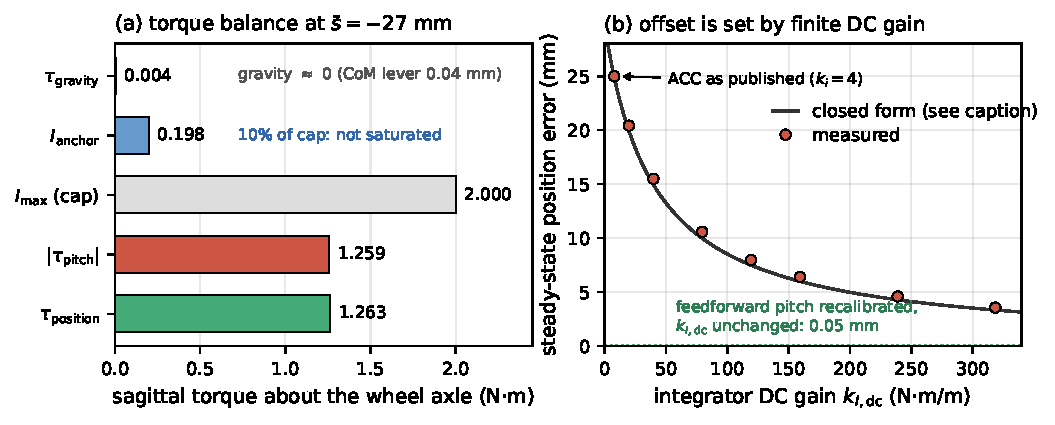
\includegraphics[width=\linewidth]{figures/parking_offset.pdf}
    \caption{Static torque balance of the sagittal parking offset.
    (a) Measured sagittal torques at the $\bar{s}{=}\SI{-27}{mm}$ parking point.
    The gravity moment about the wheel axle is \SI{0.0040}{Nm} and the anchor
    integral sits at \SI{10}{\percent} of its clamp, so the offset is neither
    gravity-driven nor a saturation artifact; the balance is between the
    pitch and position loops.
    (b) Steady-state position error against integrator DC gain
    $k_{I,\text{dc}}$ of Eq.~\eqref{eq:kidc}, swept over $k_i\in[4,160]$ at
    fixed leak. The curve is Eq.~\eqref{eq:parking} evaluated with the
    baseline $\tau_{\text{pitch}}$; using each run's own measured
    $\tau_{\text{pitch}}$ the closed form tracks all twelve gain and height
    points to within \SI{0.92}{\percent}. The dotted line is the same
    controller with the feedforward pitch reference recalibrated and
    $k_{I,\text{dc}}$ left unchanged.}
    \label{fig:parking}
\end{figure}

\subsection{Validation across a forty-fold gain sweep}

Sweeping $k_i$ from \num{4} to \num{160} at fixed leak moves $k_{I,\text{dc}}$
over $40{\times}$ and the offset follows Eq.~\eqref{eq:parking} throughout
(Fig.~\ref{fig:parking}b):

\begin{center}\footnotesize
\begin{tabular}{rrrrr}
\hline
$k_i$ & $k_{I,\text{dc}}$ & $e$ meas. & $e$ pred. & window jitter \\
 & (Nm/m) & (mm) & (mm) & (mm) \\
\hline
\textbf{4} & \textbf{7.96} & \textbf{-24.99} & \textbf{-24.87} & \textbf{0.298} \\
10 & 19.90 & -20.42 & -20.34 & 0.302 \\
20 & 39.80 & -15.49 & -15.54 & 0.147 \\
40 & 79.60 & -10.57 & -10.67 & 0.208 \\
60 & 119.40 & -7.96 & -8.01 & 0.168 \\
80 & 159.20 & -6.40 & -6.41 & 0.094 \\
120 & 238.80 & -4.59 & -4.58 & 0.114 \\
160 & 318.40 & -3.56 & -3.56 & 0.066 \\
\hline
\end{tabular}
\end{center}

Steadiness improves monotonically with $k_i$ over this range rather than
degrading, which is the opposite of the integral/steadiness trade-off measured
at $k_i{=}0$ in Table~\ref{tab:standing} and indicates that the $3{\times}$
steadiness cost reported there is paid at the first newton-metre of integral
authority, not progressively. Every entry above is measured on clean sensing
with no actuator delay; Section~\ref{sec:parking_ki_cost} shows that this is exactly
the condition under which raising $k_i$ looks free.

\subsection{Why the gain is not raised: the noise--delay cost}
\label{sec:parking_ki_cost}

The sweep above and the push protocol below both make $k_i{=}160$ look free:
the offset falls by \SI{79.5}{\percent}, clean-idle jitter improves, and
neither $F_{\min}$ nor $F_{\text{med}}$ moves. Those three probes share a
blind spot---all are run on clean sensing, and the push probe is a large
transient rather than a sustained small one. Re-running the two cells of
Table~\ref{tab:robustness} that combine medium sensor noise with actuator
delay, at $N{=}20$ per cell and identical seeds across arms, prices the change:

\begin{center}\footnotesize
\begin{tabular}{rrrrrl}
\hline
$k_i$ & $k_{I,\text{dc}}$ & $\bar{s}$ & offset & falls & Fisher \\
 & (Nm/m) & (mm) & removed & (of 40) & vs.\ $k_i{=}4$ \\
\hline
\textbf{4} & \textbf{7.96} & \textbf{-26.96} & \textbf{---} & \textbf{7} & \textbf{---} \\
20 & 39.80 & -17.47 & \SI{35.2}{\percent} & 13 & $p{=}0.196$ \\
40 & 79.60 & -12.55 & \SI{53.5}{\percent} & 10 & $p{=}0.586$ \\
80 & 159.20 & -8.37 & \SI{68.9}{\percent} & 14 & $p{=}0.126$ \\
160 & 318.40 & -5.53 & \SI{79.5}{\percent} & 17 & $p{=}0.027$ \\
\hline
\end{tabular}
\end{center}

A Cochran--Armitage trend test on $\log_2 k_i$ gives $z{=}2.34$, $p{=}0.019$:
the fall rate rises with integral gain across the sweep, and pooling every
arm above the shipped setting gives \num{54} falls in \num{160} against
\num{7} in \num{40} ($p{=}0.055$). Because the cost is graded rather than a
threshold, selecting the largest gain that is not individually significant
would be an artifact of sample size---$k_i{=}40$ carries $p{=}0.59$ only
because \num{40} trials cannot separate \SI{17.5}{\percent} from
\SI{25}{\percent}. Zero-delay cells stay clean at every gain, and the idle,
push, flight, terrain and rate-limit metrics are flat across the sweep, so
the regression is specific to noise and delay \emph{together}. One trap is
worth naming: the idle column of Table~\ref{tab:robustness} averages
survivors only, so in these two cells the higher-gain arms report
\emph{better} idle numbers while falling more often.

The mechanism follows from Eq.~\eqref{eq:leaky}. The leaky integrator has
transfer function $k_i\Delta t/(\lambda + s\Delta t)$: a DC gain of
$k_i\Delta t/\lambda$ and a corner at $\lambda/\Delta t\approx\SI{0.5}{rad/s}$.
Raising $k_i$ scales the response at \emph{every} frequency, so it lifts
mid-band gain---with the \SI{90}{\degree} lag of an integrator---in precisely
the band where the \SI{10}{ms} actuator delay of those cells has already
consumed the phase margin. Lowering $\lambda$ raises DC gain alone, leaving mid-band
untouched, but costs the memory horizon instead (next subsection). Neither
single parameter separates the two roles; doing so requires a lead-compensated
or explicitly bandwidth-limited integrator, which is a structural change to a
controller whose present form is qualified over a \num{48}-scenario suite, and
is left as future work.

\subsection{The leak sets memory, not accuracy}

Because $k_{I,\text{dc}}$ depends on both $k_i$ and $\lambda$, reducing the
leak also raises DC gain---but it is the wrong knob. Cutting
$\lambda$ from \num{5e-3} to \num{5e-4} raises $k_{I,\text{dc}}$ to
\SI{79.96}{Nm/m} and does reduce the offset to \SI{-16.31}{mm}, but window
jitter degrades from \SI{0.298}{mm} to \SI{3.463}{mm}, a factor of \num{12},
and the measured error (\SI{-14.34}{mm}) does not reach its DC prediction
(\SI{-10.41}{mm}) because the forgetting time constant
$\tau{=}\Delta t/\lambda$ has grown to \SI{20}{s} and no longer settles inside
the measurement window. Since $\tau$ is independent of $k_i$, the two
parameters separate cleanly: $k_i$ sets DC gain, $\lambda$ sets the memory
horizon. The shipped pair is chosen on that basis. $\lambda{=}\num{5e-3}$ fixes
a \SI{2}{s} forgetting time, which is what keeps the integral inside its
measurement window; $k_i{=}\num{4}$ is then set not for clean-idle steadiness,
which the gain sweep shows is flat in $k_i$, but for margin against the
noise-plus-delay conjunction quantified in Section~\ref{sec:parking_ki_cost}. The
accuracy consequence of that pair is the \SI{27}{mm} offset, and it is the price
of the memory horizon rather than of the gain.

\subsection{Two measured corrections and their cost}

The height dependence of the calibration error was checked on the five
posture-calibrated height variants, applying the correction measured at each
point. The nominal row is $N{=}10$ under the full idle protocol; the four
off-nominal heights are single trials, whose run-to-run spread the nominal
row bounds at \SI{0.011}{mm} SD:

\begin{center}\footnotesize
\begin{tabular}{rrrrr}
\hline
$h$ (m) & correction & $\bar{s}$ before & $\bar{s}$ after & reduction \\
 & (\SI{}{\degree}) & (mm) & (mm) & \\
\hline
0.394 & $-1.622$ & $-28.77$ & $-1.16$ & \SI{96.0}{\percent} \\
0.399 & $-1.974$ & $-34.53$ & $-1.20$ & \SI{96.5}{\percent} \\
\textbf{0.404} & $\mathbf{-1.461}$ & $\mathbf{-26.96}$ & $\mathbf{-2.02}$ & \textbf{\SI{92.5}{\percent}} \\
0.409 & $-0.943$ & $-19.29$ & $-2.83$ & \SI{85.3}{\percent} \\
0.414 & $-1.295$ & $-25.11$ & $-2.92$ & \SI{88.4}{\percent} \\
\hline
\end{tabular}
\end{center}

The controller's own position error falls to ${\leq}\SI{0.12}{mm}$ at every
height and the anchor integral to \SI{0.4}{\percent} of its clamp; what remains
is the \SIrange{1}{3}{mm} frame-convention gap. The required correction is not
a constant (it spans \SIrange{0.94}{1.97}{\degree} over \SI{2}{cm}), so this is
a per-height recalibration of the feedforward map rather than a single scalar.

Both corrections were then put through the full push protocol of
Section~\ref{sec:push} ($N{=}10$ repetitions $\times$ 8 bearings, binary search over
\SIrange{10}{160}{N} at \SI{5}{N} tolerance; Welch's $t$ against the published
arm):

\begin{center}\footnotesize
\begin{tabular}{lrr}
\hline
Arm & $F_{\min}$ (N) & $F_{\text{med}}$ (N) \\
\hline
ACC as published ($k_i{=}4$) & 82.8(10) & 116.8(47) \\
$k_i{=}40$ & 81.8(18)\,\,$p{=}0.14$ & 116.8(70)\,\,$p{=}0.98$ \\
$k_i{=}160$ & 81.9(27)\,\,$p{=}0.32$ & 115.3(36)\,\,$p{=}0.43$ \\
Feedforward pitch recalibrated & 82.5(12)\,\,$p{=}0.55$ & 112.4(49)\,\,$p{=}0.05$ \\
\hline
\end{tabular}
\end{center}

The published arm reproduces the weakest bearing of Section~\ref{sec:push}
(\SI{82.8}{N} here against \SI{82.3}{N} there, $\Delta{<}\SI{0.5}{N}$ on
independent seeds), validating the harness. Raising $k_i$ by $40{\times}$
costs nothing measurable on either push statistic and removes \SI{79.5}{\percent}
of the offset; the feedforward recalibration removes \SI{92.5}{\percent} and
leaves $F_{\min}$ unchanged, but shows a \SI{4.5}{N} (\SI{3.8}{\percent})
reduction in $F_{\text{med}}$ at $p{=}0.051$, which at this sample size we
report as unresolved rather than as null.

Neither correction is promoted into the shipped profile, and in the $k_i$ case
the reason is not evidence-base consistency but a measured regression: the
push protocol is blind to the failure mode that gain change introduces, which
appears only when sustained sensor noise and actuator delay act together
(Section~\ref{sec:parking_ki_cost}). This is the substantive result of the appendix.
The \SI{27}{mm} offset is not an unexamined residual, nor a defect awaiting a
constant change; it is the position error that a deliberately leaky,
deliberately low-gain integrator must pay in exchange for a \SI{2}{s}
forgetting horizon and for phase margin against delay. Both alternatives were
measured across the full evaluation suite rather than on the accuracy metric
alone, which is what exposed the price. The feedforward recalibration remains
the more promising route, since its cost is confined to one borderline
statistic; resolving that at a larger sample, and testing whether a
bandwidth-limited integrator can raise DC gain without raising mid-band gain,
are the two concrete steps toward closing this limitation.

\begin{thebibliography}{99}
\setlength{\itemsep}{0pt}
\setlength{\parsep}{0pt}
\setlength{\topsep}{0pt}

\bibitem{klemm2019ascento}
V.~Klemm, et al., Ascento: a two-wheeled jumping robot, in: Proc. IEEE Int.
Conf. Robot. Autom. (ICRA), 2019.

\bibitem{klemm2020lqrwbc}
V.~Klemm, A.~Morra, L.~Gulich, et al., LQR-assisted whole-body control of a
wheeled bipedal robot with kinematic loops, IEEE Robot. Autom. Lett. 5 (2)
(2020) 3745--3752.

\bibitem{skater2024}
Y.~Wang, T.~Chen, X.~Rong, G.~Zhang, Y.~Li, Y.~Xin, Design and control of
SKATER: a wheeled-bipedal robot with high-speed turning robustness and terrain
adaptability, IEEE/ASME Trans. Mechatron. 30 (2) (2025) 1310--1321.

\bibitem{hwangbo2019rl}
J.~Hwangbo, J.~Lee, A.~Dosovitskiy, D.~Bellicoso, V.~Tsounis, V.~Koltun,
M.~Hutter, Learning agile and dynamic motor skills for legged robots, Sci.
Robot. 4 (26) (2019) eaau5872.

\bibitem{schulman2017ppo}
J.~Schulman, F.~Wolski, P.~Dhariwal, A.~Radford, O.~Klimov, Proximal policy
optimization algorithms, arXiv preprint arXiv:1707.06347 (2017).

\bibitem{johannink2019residual}
T.~Johannink, S.~Bahl, A.~Nair, J.~Luo, A.~Kumar, M.~Loskyll, J.A.~Ojea,
E.~Solowjow, S.~Levine, Residual reinforcement learning for robot control, in:
Proc. IEEE Int. Conf. Robot. Autom. (ICRA), 2019, pp. 6023--6029.

\bibitem{silver2018residual}
T.~Silver, K.~Allen, J.~Tenenbaum, L.~Kaelbling, Residual policy learning,
arXiv preprint arXiv:1812.06298 (2018).

\bibitem{boston_dynamics_handle2017}
Boston Dynamics, Introducing Handle, YouTube video, March 2017.
\url{https://youtu.be/-7xvqQeoA8c}.

\bibitem{bjelonic2019wheeled}
M.~Bjelonic, C.D.~Bellicoso, Y.~de~Viragh, D.~Sako, F.D.~Tresoldi,
F.~Jenelten, M.~Hutter, Keep rollin'---whole-body motion control and planning
for wheeled quadrupedal robots, IEEE Robot. Autom. Lett. 4 (2) (2019)
2116--2123.

\bibitem{zhang2022ollie}
J.~Zhang, S.~Wang, H.~Wang, J.~Lai, Z.~Bing, Y.~Jiang, Y.~Zheng, Z.~Zhang, An
adaptive approach to whole-body balance control of wheel-bipedal robot Ollie,
in: Proc. IEEE/RSJ Int. Conf. Intell. Robots Syst. (IROS), 2022, pp.
12835--12842.

\bibitem{bjelonic2021mpc}
M.~Bjelonic, R.~Grandia, O.~Harley, C.~Galliard, S.~Zimmermann, M.~Hutter,
Whole-body MPC and online gait sequence generation for wheeled-legged robots,
in: Proc. IEEE/RSJ Int. Conf. Intell. Robots Syst. (IROS), 2021, pp.
8388--8395.

\bibitem{diablo2024}
D.~Liu, F.~Yang, X.~Liao, X.~Lyu, DIABLO: a 6-DoF wheeled bipedal robot
composed entirely of direct-drive joints, in: Proc. IEEE/RSJ Int. Conf. Intell.
Robots Syst. (IROS), 2024, pp. 3605--3612.

\bibitem{whleaper2024}
Y.~Zhu, S.~He, Z.~Qi, Z.~Yong, Y.~Qin, J.~Chen, Whleaper: a 10-DOF flexible
bipedal wheeled robot, in: Proc. IEEE/RSJ Int. Conf. Intell. Robots Syst.
(IROS), 2024, pp. 11272--11277.

\bibitem{zhang2025residualwbr}
J.~Zhang, B.~Lu, H.~Cao, Y.~Fang, Hybrid balance control for wheeled bipedal
robot via residual reinforcement learning optimization, in: Proc. 10th
Asia-Pac. Conf. Intell. Robot Syst. (ACIRS), 2025, pp. 59--66.

\bibitem{cascade_standard}
K.J.~\AA{}str\"{o}m, T.~H\"{a}gglund, PID Controllers: Theory, Design, and
Tuning, second ed., Instrument Society of America, 1995.

\bibitem{herzog2016wbc}
A.~Herzog, N.~Rotella, S.~Mason, F.~Grimminger, S.~Schaal, L.~Righetti,
Momentum control with hierarchical inverse dynamics on a torque-controlled
humanoid, Auton. Robots 40 (3) (2016) 473--491.

\bibitem{bellicoso2018wbc}
C.D.~Bellicoso, F.~Jenelten, C.~Gehring, M.~Hutter, Dynamic locomotion through
online nonlinear motion optimization for quadrupedal robots, IEEE Robot. Autom.
Lett. 3 (3) (2018) 2261--2268.

\bibitem{escande2014hqp}
A.~Escande, N.~Mansard, P.-B.~Wieber, Hierarchical quadratic programming: fast
online humanoid-robot motion generation, Int. J. Robot. Res. 33 (7) (2014)
1006--1028.

\bibitem{gain_scheduling_survey}
W.J.~Rugh, J.S.~Shamma, Research on gain scheduling, Automatica 36 (10) (2000)
1401--1425.

\bibitem{leith2000gainsched}
D.J.~Leith, W.E.~Leithead, Survey of gain-scheduling analysis and design, Int.
J. Control 73 (11) (2000) 1001--1025.

\bibitem{shinskey1996}
F.G.~Shinskey, Process Control Systems: Application, Design, and Tuning, fourth
ed., McGraw-Hill, 1996.

\bibitem{astrom2005advanced}
K.J.~\AA{}str\"{o}m, T.~H\"{a}gglund, Advanced PID Control, ISA, 2006.

\bibitem{liberzon2003switching}
D.~Liberzon, Switching in Systems and Control, Birkh\"{a}user, 2003.

\bibitem{hespanha2003hysteresis}
J.P.~Hespanha, D.~Liberzon, A.S.~Morse, Hysteresis-based switching algorithms
for supervisory control of uncertain systems, Automatica 39 (2) (2003)
263--272.

\bibitem{liu2024review}
X.~Liu, Y.~Sun, S.~Wen, K.~Cao, Q.~Qi, X.~Zhang, H.~Shen, G.~Chen, J.~Xu,
A.~Ji, Development of wheel-legged biped robots: a review, J. Bionic Eng. 21
(2) (2024) 607--634.

\bibitem{ohnishi1993dob}
K.~Ohnishi, M.~Shibata, T.~Murakami, Motion control for advanced mechatronics,
IEEE/ASME Trans. Mechatron. 1 (1) (1996) 56--67.

\bibitem{chen2000dob}
W.-H.~Chen, D.J.~Ballance, P.J.~Gawthrop, J.~O'Reilly, A nonlinear disturbance
observer for robotic manipulators, IEEE Trans. Ind. Electron. 47 (4) (2000)
932--938.

\bibitem{han2009adrc}
J.~Han, From PID to active disturbance rejection control, IEEE Trans. Ind.
Electron. 56 (3) (2009) 900--906.

\bibitem{feng2023lqradrc}
X.~Feng, S.~Liu, Q.~Yuan, J.~Xiao, D.~Zhao, Research on wheel-legged robot
based on LQR and ADRC, Sci. Rep. 13 (2023) 15122.

\bibitem{astrom1989windup}
K.J.~\AA{}str\"{o}m, L.~Rundqwist, Integrator windup and how to avoid it, in:
Proc. Am. Control Conf. (ACC), 1989, pp. 1693--1698.

\bibitem{kothare1994antiwindup}
M.V.~Kothare, P.J.~Campo, M.~Morari, C.N.~Nett, A unified framework for the
study of anti-windup designs, Automatica 30 (12) (1994) 1869--1883.

\bibitem{tarbouriech2009aw}
S.~Tarbouriech, M.~Turner, Anti-windup design: an overview of some recent
advances and open problems, IET Control Theory Appl. 3 (1) (2009) 1--19.

\bibitem{englsberger2015dcm}
J.~Englsberger, C.~Ott, A.~Albu-Sch\"{a}ffer, Three-dimensional bipedal walking
control based on divergent component of motion, IEEE Trans. Robot. 31 (2)
(2015) 355--368.

\bibitem{pratt2006capturepoint}
J.~Pratt, J.~Carff, S.~Drakunov, A.~Goswami, Capture point: a step toward
humanoid push recovery, in: Proc. IEEE-RAS Int. Conf. Humanoid Robots, 2006,
pp. 200--207.

\bibitem{roscia2023flight}
F.~Roscia, A.~Cumerlotti, A.~Del~Prete, C.~Semini, M.~Focchi, Orientation
control system: enhancing aerial maneuvers for quadruped robots, Sensors 23 (3)
(2023) 1234.

\bibitem{chamorro2024stairclimbing}
S.~Chamorro, V.~Klemm, M.~de~la~Iglesia~Valls, C.~Pal, R.~Siegwart,
Reinforcement learning for blind stair climbing with legged and wheeled-legged
robots, in: Proc. IEEE Int. Conf. Robot. Autom. (ICRA), 2024, pp. 8081--8087.

\bibitem{legged_terrain_extero}
M.~Hutter, et al., ANYmal---toward legged robots for harsh environments, Adv.
Robot. 31 (17) (2017) 918--931.

\bibitem{fankhauser2018rough}
P.~Fankhauser, M.~Bjelonic, C.D.~Bellicoso, T.~Miki, M.~Hutter, Robust
rough-terrain locomotion with a quadrupedal robot, in: Proc. IEEE Int. Conf.
Robot. Autom. (ICRA), 2018, pp. 5761--5768.

\bibitem{lee2020challenging}
J.~Lee, J.~Hwangbo, L.~Wellhausen, V.~Koltun, M.~Hutter, Learning quadrupedal
locomotion over challenging terrain, Sci. Robot. 5 (47) (2020) eabc5986.

\bibitem{miki2022perceptive}
T.~Miki, J.~Lee, J.~Hwangbo, L.~Wellhausen, V.~Koltun, M.~Hutter, Learning
robust perceptive locomotion for quadrupedal robots in the wild, Sci. Robot. 7
(62) (2022) eabk2822.

\bibitem{blind_terrain_proprio}
G.~Bledt, et al., Contact model fusion for event-based locomotion in
unstructured terrains, in: Proc. IEEE Int. Conf. Robot. Autom. (ICRA), 2018,
pp. 4399--4406.

\bibitem{bellicoso2016terrain}
C.D.~Bellicoso, C.~Gehring, J.~Hwangbo, P.~Fankhauser, M.~Hutter,
Perception-less terrain adaptation through whole body control and hierarchical
optimization, in: Proc. IEEE-RAS Int. Conf. Humanoid Robots (Humanoids), 2016,
pp. 558--564.

\bibitem{camurri2017contact}
M.~Camurri, M.~Fallon, S.~Bazeille, A.~Radulescu, V.~Barasuol, D.G.~Caldwell,
C.~Semini, Probabilistic contact estimation and impact detection for state
estimation of quadruped robots, IEEE Robot. Autom. Lett. 2 (2) (2017)
1023--1030.

\bibitem{hyon2007gated}
S.-H.~Hyon, G.~Cheng, Gravity compensation and full-body balancing for humanoid
robots, in: Proc. IEEE-RAS Int. Conf. Humanoid Robots, 2006, pp. 214--221.

\bibitem{mujoco}
E.~Todorov, T.~Erez, Y.~Tassa, MuJoCo: a physics engine for model-based
control, in: Proc. IEEE/RSJ Int. Conf. Intell. Robots Syst. (IROS), 2012, pp.
5026--5033.

\bibitem{grasser2002joe}
F.~Grasser, A.~D'Arrigo, S.~Colombi, A.C.~Rufer, JOE: a mobile, inverted
pendulum, IEEE Trans. Ind. Electron. 49 (1) (2002) 107--114.

\bibitem{pathak2005wip}
K.~Pathak, J.~Franch, S.K.~Agrawal, Velocity and position control of a wheeled
inverted pendulum by partial feedback linearization, IEEE Trans. Robot. 21 (3)
(2005) 505--513.

\bibitem{grimminger2020torque}
F.~Grimminger, A.~Meduri, M.~Khadiv, J.~Viereck, M.~W\"{u}thrich,
L.~Wellhausen, et al., An open torque-controlled modular robot architecture for
legged locomotion research, IEEE Robot. Autom. Lett. 5 (2) (2020) 3650--3657.

\bibitem{tobin2017domainrand}
J.~Tobin, R.~Fong, A.~Ray, J.~Schneider, W.~Zaremba, P.~Abbeel, Domain
randomization for transferring deep neural networks from simulation to the real
world, in: Proc. IEEE/RSJ Int. Conf. Intell. Robots Syst. (IROS), 2017, pp.
23--30.

\bibitem{peng2018dynrand}
X.B.~Peng, M.~Andrychowicz, W.~Zaremba, P.~Abbeel, Sim-to-real transfer of
robotic control with dynamics randomization, in: Proc. IEEE Int. Conf. Robot.
Autom. (ICRA), 2018, pp. 3803--3810.

\bibitem{bryson1975optimal}
A.E.~Bryson, Y.-C.~Ho, Applied Optimal Control: Optimization, Estimation and
Control, revised ed., Hemisphere Publishing, 1975.

\bibitem{stellato2020osqp}
B.~Stellato, G.~Banjac, P.~Goulart, A.~Bemporad, S.~Boyd, OSQP: an operator
splitting solver for quadratic programs, Math. Program. Comput. 12 (4) (2020)
637--672.

\end{thebibliography}

\end{document}
